%% ============================================================
%%  jmlr-paper-main.tex
%%  HypatiaX: Hybrid Symbolic-Neural Framework for
%%  Extrapolation-Reliable Analytical Discovery
%%  MAIN PAPER — JMLR submission (extended, v3.0 benchmark)
%%  Author: Ruperto Pedro Bonet Chaple
%%  Built: April 2026
%%  Companion files:
%%    supp_routing_improvements.tex  — Supplementary A
%%    supp_benchmark_report.tex      — Supplementary B
%% ============================================================

\documentclass[twoside,11pt]{article}

%% ── JMLR house style ────────────────────────────────────────
\usepackage{jmlr2e}

%% ── Core maths & fonts ──────────────────────────────────────
%% NOTE: amsthm is deliberately NOT loaded. jmlr2e.sty already
%% defines proof/theorem/lemma/proposition/remark/corollary/
%% definition (see jmlr2e.sty "PROOF, THEOREM, and FRIENDS" section)
%% using plain-LaTeX \newtheorem/\newenvironment. Loading amsthm on
%% top of that redefines the kernel theorem-optional-argument
%% machinery and breaks jmlr2e's already-declared environments
%% (symptom: "No counter 'Definition' defined" on
%% \begin{definition}[Title]). Neither this file nor the
%% supplementary files use any amsthm-only feature (\theoremstyle,
%% \qedhere, \newtheorem*), so it isn't needed.
\usepackage{amsmath,amssymb,amsfonts}

\usepackage{bm}
\usepackage{microtype}
\microtypesetup{expansion=true}

%% ── Figures, tables, algorithms ─────────────────────────────
\usepackage{graphicx}
\usepackage{float}
%%adjustbox-removed
\usepackage{booktabs}
\usepackage{caption}
\usepackage{subcaption}
\usepackage{silence}
\WarningFilter{caption}{Unknown}
\usepackage{algorithm}
\usepackage{algpseudocode}
\usepackage{multirow}
\usepackage{threeparttable}
\usepackage{longtable}
\usepackage{tabularx}
\usepackage{makecell}
\usepackage{colortbl}
\usepackage{array}

%% ── Typography & misc ───────────────────────────────────────
\usepackage{enumitem}
\usepackage{hyperref}
\usepackage{xcolor}

\graphicspath{{figures/}{../figures/}{hypatiax/data/results/figures/}}
% Accept pdf, png, jpg in that priority order — figures_deploy produces .png
% when generate_figures.py writes .png only; pdflatex accepts all three.
\DeclareGraphicsExtensions{.pdf,.PDF,.png,.PNG,.jpg,.JPG}

%% ── Colours ─────────────────────────────────────────────────
\definecolor{passgreenBg}{RGB}{204,255,204}
\definecolor{warnAmberBg}{RGB}{255,235,180}
\definecolor{failredBg}{RGB}{255,204,204}

%% ── Placeholder for missing data ────────────────────────────
\newcommand{\TODO}{\textcolor{red}{[TODO]}}

%% ── Math macros ─────────────────────────────────────────────
\newcommand{\Rsq}{R^{2}}
\newcommand{\Rtrain}{R^{2}_{\mathrm{train}}}
\newcommand{\Rtest}{R^{2}_{\mathrm{test}}}
\newcommand{\Redge}{R^{2}_{\mathrm{edge}}}
\newcommand{\II}{\mathrm{II}}
\newcommand{\abs}[1]{\left|#1\right|}
\newcommand{\wLLM}{w_{\mathrm{LLM}}}
\newcommand{\wNN}{w_{\mathrm{NN}}}
\newcommand{\R}{\mathbb{R}}
\newcommand{\verified}[1]{\textcolor{blue!60!black}{#1}}

%% ── Theorem environments ────────────────────────────────────
%% theorem/definition/proposition/corollary/remark/lemma are ALL
%% already defined unconditionally by jmlr2e.sty (identical names,
%% shared "theorem" counter) — see jmlr2e.sty lines 388-394. They
%% must NOT be redeclared here; only result/finding/constraint are
%% genuinely new and not touched by jmlr2e.
\newtheorem{result}{Empirical Result}
\newtheorem{finding}{Empirical Finding}
\newtheorem{constraint}{System Constraint}
\newenvironment{demonstration}{\begin{trivlist}\item[\hskip\labelsep\textbf{Empirical Demonstration.}]}{\end{trivlist}}
\newenvironment{argument}{\begin{trivlist}\item[\hskip\labelsep\textbf{Theoretical Argument.}]}{\end{trivlist}}

% =============================================================================
\title{HypatiaX: A Hybrid Symbolic-Neural Framework for
  Extrapolation-Reliable Analytical Discovery}

\author{R.~P.~Bonet Chaple}

\date{2026}

% =============================================================================
\begin{document}
\raggedbottom

\jmlrheading{1}{2026}{1-99}{1/26}{4/26}{Bonet Chaple}
\ShortHeadings{HypatiaX: A Hybrid Symbolic-Neural Framework for Extrapolation-Reliable Analytical Discovery}{Bonet Chaple}
\firstpageno{1}

\title{HypatiaX: A Hybrid Symbolic-Neural Framework for
  Extrapolation-Reliable Analytical Discovery}

\author{Ruperto Pedro Bonet Chaple\\
  \texttt{ruperto.bonet@modelphysmat.com}\\
  Independent Researcher, London, United Kingdom
}

\editor{}

\maketitle

% ── Author note on numerical accuracy ────────────────────────────────────────
\begin{center}
\fbox{\parbox{0.88\textwidth}{%
\small\textbf{Note on data provenance and prior-draft corrections.}
Two claims from early drafts of this paper did not survive verification
against the raw per-task result files and are not repeated in this
version: a ``73\,\% runtime reduction'' ($3.7\times$ speedup) and a
subsequently reported $1.73\times$/$1.64\times$ speedup, both for
HypatiaX over the neural-network baseline. The verified result is the
opposite: across the five 74-task seed files held in the repository ($370$ task
runs audited), the hybrid system is
\emph{slower} than the pure neural-network baseline on every seed,
by a factor of $3.8\times$ to $11.2\times$ on mean time,
whether measured over all tasks or over LLM-routed tasks only
(Table~\ref{tab:timing_full}, \S\ref{sec:timing}).

All seed-42 DeFi figures in this paper (the near-perfect-rate and
decision-attribution-bug analysis of \S\ref{sec:hybrid-attribution-bug},
Table~\ref{tab:difficulty}, and Table~\ref{tab:hybrid-bug-breakdown}) are
computed from \texttt{hypatiax\_defi\_benchmark\_v3\_results\_seed42.json}
as it currently exists in the repository (canonical location
\texttt{hypatiax/data/results/comparison\_results/noise-noiseless/noiseless/defi};
identical copies under \texttt{hypatiax-dev/data\_exp} and \texttt{data\_old};
md5 \texttt{cbf503d0b3985b4c1bccf7ed18e0316b}). This file's raw figures
--- \texttt{hybrid.test\_r2}$>0.99$ on 67/74 tasks (90.5\,\%),
\texttt{pure\_llm.success} on 45/74 (60.8\,\%), and 5 pure-LLM
catastrophic failures ($\Rsq<-10$) --- match this paper's own headline
raw numbers exactly, and are the basis for every corrected figure
reported below and in \S\ref{sec:hybrid-attribution-bug}: 44/74 (59.5\,\%)
corrected near-perfect rate, tied with pure LLM tier-by-tier, and 23
fabricated successes (3 easy / 11 medium / 9 hard), not the 8 cited in
earlier drafts. Two other v3-labelled seed-42 files exist in the
repository (in \texttt{hypatiax-dev/data}/\texttt{data\_dev}/\texttt{data\_last},
md5 \texttt{89037935469176741a5fb4479f2c725f}, from which an earlier version of this paper was computed, and in
\texttt{hypatiax/data\_old}) with slightly different task-level results
(73/74 and 67/74 raw \texttt{hybrid.success} respectively, against 72/74
above); all three give a corrected near-perfect rate in the same
58--61\,\% band and a fabricated-success count of 22--23, so the
qualitative finding --- HypatiaX ties, rather than beats, pure LLM on
this benchmark once the attribution bug is corrected --- does not depend
on which of the three is used. Separately, a fourth-generation
(\texttt{v4}) result file with a different, more complex router now
occupies the \texttt{hypatiax/data} path the repository's own README
designates as source-of-truth; that file uses a materially different
architecture from the three-way (Pure LLM / Neural Network / Hybrid)
system this paper describes and is not used anywhere in this paper. \textbf{Update (2026-09-28):} every cell of
Table~\ref{tab:main_results} has now been recomputed directly from this
file under the paper's own metric definitions (\S\ref{sec:setup_metrics}).
The earlier Pure~LLM and Neural~MLP rows did not reproduce and have been
replaced; the Hybrid row is shown both uncorrected (the pipeline's
self-report) and corrected for the attribution bug.}}
\end{center}
\vspace{0.5em}

% =============================================================================
\begin{abstract}
The hardest test of a formula-recovery system is not interpolation accuracy but
out-of-distribution extrapolation.  Two cases from our benchmark make this stark.
On Arrhenius, PySR-only collapses catastrophically at $5\times$ the
training range (far-$\Rsq = -12.56$); HypatiaX anchors the search via an
LLM warm-start and recovers the correct functional form (far-$\Rsq = 0.90$),
a genuine rescue rather than a shared failure. On Portfolio
Variance, PySR-only fails on all five tested random seeds; HypatiaX recovers
the exact closed-form formula ($\Rsq=1.000$ at $5\times$ training range) on
seeds 777 and 2024, and is close to or somewhat better than PySR-only on
seeds 42 and 123. We also document an honest failure mode on the opposite
side: on Michaelis-Menten, HypatiaX's extrapolation evaluation never
completed (no value recorded near, medium, or far), while PySR-only
succeeded (far-$\Rsq = 0.65$); and on Portfolio Variance seed~99, HypatiaX
underperforms PySR-only at far extrapolation. These phenomena---selective
rescue, selective degradation, and outright missing evaluations---are the
empirical core of this paper.

We introduce \textbf{HypatiaX}, a hybrid symbolic--neural framework that
addresses this through a five-stage routing and ensembling mechanism---trust
gating, transcendental complexity detection, neural degradation probing,
out-of-distribution detection, and uncertainty-weighted ensembling---that
dynamically selects between LLM symbolic output and a residual neural network
using training-data diagnostics alone.  The key insight is that the two paradigm
failure modes are complementary: routing between them eliminates catastrophic
failures while preserving the accuracy ceiling of the stronger component.

On a benchmark of 74 DeFi mathematical tasks under a 40\,\%/60\,\% extrapolation split (the released result files do not record whether the single-axis or PCA-directed variant was used), a standalone neural MLP achieves
median test $\Rsq = -0.69$, and a pure LLM baseline suffers 5 catastrophic
failures ($\Rsq < -10$) while achieving only 59.5\,\% near-perfect recovery.
Neither paradigm alone is sufficient.

Across all 74 tasks, HypatiaX's own reported output shows a median test
$\Rsq$ of $1.00$ and a near-perfect success rate ($\Rsq>0.99$) of
\textbf{90.5\,\%}\footnote{This figure is computed from the hybrid system's
own reported \texttt{success}/$\Rsq$ fields without cross-checking the
routing decision against the actual success of the sub-method it names.
See \S\ref{sec:hybrid-attribution-bug}.}, an apparent $+28.3$ percentage
point gain over the LLM baseline and $+85.1$\,pp over the neural network.
\textbf{Neither figure survives attribution correction.} Once the routing
decision is cross-checked against the sub-method it actually names, the
corrected near-perfect rate is $59.5\,\%$ ($44/74$) --- \emph{identical} to
the pure LLM baseline's own rate on the same 74 tasks ($44/74$), and
against the $0/74$ neural-network baseline. We similarly re-examined the
claim that HypatiaX \textbf{eliminates catastrophic failures}
($\Rsq<-10$): its own reported output shows zero, but checked against the
sub-method actually selected on each task, catastrophic failures occur at
the same rate as pure LLM alone ($6/74$ in both
cases)\footnote{The failure is masked, not eliminated: a sub-method
(typically the LLM proposal) that itself failed catastrophically is
masked on some tasks (e.g.\ \texttt{pure\_llm.test\_r2} $\approx -141{,}000$
on Loan-to-Value), while the hybrid system's own accounting reports
\texttt{success=True}, $\Rsq \approx 1.0$ regardless. Full per-task detail
in \S\ref{sec:hybrid-attribution-bug}.}. \textbf{We therefore do not find a
corrected accuracy or catastrophic-failure-avoidance advantage of the
hybrid system over its own LLM component on this benchmark.} A
per-difficulty breakdown of this correction, and an attempted multi-seed
extension, are given in \S\ref{sec:hybrid-attribution-bug}; the
multi-seed extension is not currently reportable, as 4 of the 5 available
seed runs suffered majority-to-total pure-LLM execution failure (an
API/pipeline fault unrelated to model performance, not a modelling
result), leaving seed 42 as the only complete, usable run for this
comparison.
On the standard Nguyen-12 suite, rebuilt (2026-09-28) from the
consolidated CI result files
\texttt{hypatiax/data/results/extrapolation/exp3\_nguyen12\_seed42.json} and
\texttt{multi\_seed/exp3\_nguyen12\_seed\{99,123,777,2024\}\_nshards*.json}
(the files the current pipeline produces; an earlier table cited
\texttt{exp3\_nguyen12\_hybrid50v.json}, which does not exist in this
repository's history), PySR-only and HypatiaX each recover \textbf{10/12
(83.3\,\%)} equations on seed~42 at $\Rsq\ge0.9999$, and across five seeds
HypatiaX recovers \textbf{51/60 (85.0\,\%)} against \textbf{49/60 (81.7\,\%)} for
PySR-only. This replaces the earlier 12/12 (100\,\%) figure for both systems,
which does not reproduce from any file in the repository. The one structural
result is Nguyen-12 ($x^4-x^3+\tfrac12y^2-y$): HypatiaX fails it on
\emph{all five} seeds, because the LLM candidate gate rejects all eight
proposed candidates and, with \texttt{llm\_require\_valid\_guess=True}, the run aborts
before any symbolic search (PySR-only recovers it on 5/5). See
Table~\ref{tab:nguyen12} and \S\ref{sec:nguyen12}. Earlier figures
(8/12~P, 7/12~H, 4/12, and a Neural MLP baseline that was never run) remain
withdrawn.
A previously reported $1.73\times$ median speedup of HypatiaX over
neural-network inference on LLM-routed cases (68 of 74, split not recorded
--- no seed was disclosed for the original claim; two of the
five seed files in the repository route exactly 68/74, see
Table~\ref{tab:timing_full}) does
\textbf{not} reproduce: regeneration of the runtime table directly from
the raw per-task result files, across the five 74-task seed files in the
repository, shows the hybrid system
is $3.8$--$11.2\times$ \emph{slower} than the neural baseline on every
seed, never faster (see \S\ref{sec:timing}).
On a custom 30-equation benchmark spanning mechanics to quantum physics (not a subset of the AI Feynman suite), HypatiaX
passes 21/30 under a random 80/20 split and 13/30 on the held-out 60\,\% of a
PCA-directed 40\,\%/60\,\% split\footnote{Strict $\Rsq \geq 0.999999$ threshold. The random-split
figure uses the method-reported $\Rsq$; the PCA figure uses the far-region $\Rsq$ recomputed on
the held-out 60\,\%, the extrapolation measure; see \S\ref{sec:feynman30}.}, versus 0/30 for the neural
baseline on the random split. A pure-LLM baseline passes 29/30 on the random split, so this suite
shows an advantage over the neural baseline but not over the pure LLM; held-out PCA scores are
not available for the pure-LLM and hybrid-core methods because of an evaluator defect
(Section~\ref{sec:feynman30}).
Taken together, it is the individual extrapolation-rescue cases documented
above (Arrhenius, Portfolio Variance) and the 30-equation benchmark comparison
against the neural baseline --- not an aggregate near-perfect-rate or
catastrophic-failure-avoidance gain on the DeFi benchmark --- that
constitute this paper's empirically supported evidence for
\emph{reliability under distribution shift} as a property of hybrid
symbolic--neural systems.
\end{abstract}

\begin{quote}\small
\textbf{Note.} Several claims and one full table in this manuscript were
withdrawn or corrected during an internal review; each affected passage is
marked in place, with the corrected value, its provenance, and (where
applicable) the reconciliation against the original claim given directly
at that location rather than in a separate tracking document.

\medskip
\noindent\textbf{Note (hybrid decision-attribution bug).} Every
near-perfect success-rate figure for the hybrid system quoted in this
manuscript (\textbf{90.5\,\%} overall, and the \textbf{100.0\,\%
(Easy)\,/\,93.1\,\% (Medium)\,/\,76.2\,\% (Hard)} difficulty
breakdown) is computed directly from the pipeline's \texttt{hybrid.success}
/ \texttt{hybrid.test\_r2} fields \emph{without} cross-checking the
\texttt{hybrid.decision} field against the actual \texttt{success} flag of
the sub-method that decision names. Re-analysis of the underlying result
JSON (\texttt{hypatiax\_defi\_benchmark\_v3\_results\_seed42.json}) confirms
this is a real code-level bug, not evaluation noise: in 23 of 74 tasks,
\texttt{hybrid.decision} names a sub-method (always \texttt{"llm"} in this
run) whose own \texttt{test\_r2} does not exceed 0.99 for that same task,
yet \texttt{hybrid.test\_r2} still reports a near-perfect value in all 23
cases. This correction is reproducible directly from the raw benchmark JSON
by cross-checking \texttt{hybrid.decision} against the named sub-method's
own \texttt{test\_r2} field (see \S\ref{sec:hybrid-attribution-bug}).
See \S\ref{sec:hybrid-attribution-bug} for the full quantification
and corrected figures; all affected passages are marked in place with a
forward reference to that section.
\end{quote}


\tableofcontents
\newpage

% =============================================================================
\section{Introduction}
\label{sec:intro}

Extrapolation beyond the observed training distribution is a fundamental challenge
in machine learning.  In financial and decentralised-finance (DeFi) domains, the
problem is particularly acute: pricing models, risk metrics, and market-maker
invariants must generalise correctly to input regimes that may differ dramatically
from observed historical data.  A system that interpolates well but extrapolates
poorly is of limited practical value in this setting.

Two broad paradigms have been applied to mathematical function recovery in such
domains:

\paragraph{Neural network regression.}
Multilayer perceptrons and related architectures are powerful interpolators but
are known to fail systematically under distribution shift.  Even with augmentation
techniques, neural networks trained on $\mathcal{D}_{\mathrm{train}}$ do not, in
general, recover the functional form of $f$ beyond the training convex hull.  Our
benchmark confirms this: the neural MLP baseline achieves a median test $\Rsq$ of
$-0.69$ under extrapolation---worse than predicting the mean.

\paragraph{LLM-based symbolic regression.}
Large language models can, in principle, recover exact closed-form expressions from
task descriptions, achieving perfect extrapolation when the correct formula is
produced.  However, this approach exhibits a severe bimodal failure pattern: on
the single-run seed-42 evaluation of the 74-task DeFi benchmark, LLMs achieve
median test $\Rsq=1.00$ with 5 catastrophic failures ($\Rsq < -10$) out of 74
tasks.\footnote{A genuine multi-run stability sweep ($K=30$ independent
stochastic evaluations per task, as opposed to this single-run figure) was
planned and is referenced in the pipeline's own intermediate outputs, but its
raw results are not present in the released repository at the time of this
revision; the mean $\Rsq$ and instability-regime figures previously reported
here could not be reproduced and have been removed pending that data. See the
Post-Submission Report.} More importantly, a single-run evaluation---the
standard in prior work---plausibly conceals run-to-run instability on complex
transcendental tasks, though we cannot currently quantify this from verified
data (\S\ref{sec:instability_results}).

\medskip\noindent
\textbf{Central claim.}
Neither paradigm alone is sufficient.  The key insight of HypatiaX is that
these two failure modes are \emph{complementary}: neural networks fail on
the tasks where LLMs succeed (transcendental extrapolation), and LLMs fail
on the tasks where a neural network with LLM-augmented features can stabilise
performance.  A routing mechanism that dynamically selects between the two
modes---based on observable diagnostics computed from training data alone---is
\emph{designed to} eliminate catastrophic failures while preserving near-perfect
accuracy on the cases where symbolic recovery is reliable. On the DeFi
benchmark used in this paper, however, this design intent does not fully
materialise once a decision-attribution bug in the routing mechanism's own
success reporting is corrected: catastrophic failures are masked rather than
eliminated, and the corrected near-perfect rate ties, rather than beats, the
pure-LLM baseline (\S\ref{sec:hybrid-attribution-bug}). The paper's supported
evidence for the routing approach instead comes from individual
extrapolation-rescue cases and the Protocol-30 comparison
(\S\ref{sec:results}, \S\ref{sec:discussion}), not from an aggregate gain on
this benchmark.

\subsection{Contributions}\label{subsec:contributions}
\label{sec:contributions}

This paper makes the following contributions:

\begin{enumerate}[leftmargin=2em,label=(\roman*)]
  \item \textbf{HypatiaX benchmark}: a corpus of 74 closed-form DeFi tasks
    with a 40\,\%/60\,\% extrapolation split (the released result files do not record whether the single-axis or PCA-directed variant was used), together
    with a unified evaluation pipeline (HypatiaX v3.0) that corrects four
    systematic biases in prior versions (data leakage, split misconfiguration,
    formula evaluation inconsistency, and weak trust gating).

  \item \textbf{HypatiaX hybrid system}: a five-stage routing and ensembling
    mechanism---trust gating, transcendental token detection, neural degradation
    probing, OOD detection, and uncertainty-weighted ensembling---that achieves
    a \textbf{59.5\,\%} corrected near-perfect success rate ($\Rsq>0.99$) across
    all 74 tasks (44/74; the pipeline's own uncorrected figure is 90.5\,\%, 67/74,
    before removing 23 fabricated successes --- see Table~\ref{tab:hybrid-bug-breakdown}
    and \S\ref{sec:hybrid-attribution-bug})

  \item \textbf{Runtime reproducibility audit}: a mechanical, script-driven,
    script-driven regeneration of the wall-clock timing table
    directly from raw per-task result files (Table~\ref{tab:timing_full},
    Section~\ref{sec:timing}) that supersedes three earlier, unsupported
    runtime claims --- a previously circulated 73\,\% reduction claim, a
    subsequent $1.73\times$/$1.64\times$ speedup claim, and a still later
    $2.5$--$9.3\times$-slower claim that itself did not reproduce from its
    own cited source. Across the five 74-task seed files held in the
    repository ($370$ task runs audited), the hybrid
    system is found to be $3.8$--$11.2\times$ \emph{slower} than the neural
    baseline on every seed, never faster, in either the
    ``all tasks'' or ``LLM-routed-only'' framing. Restricting to only the
    tasks the hybrid system's own \texttt{decision} field routed to the LLM,
    every one of the five seed rows in Table~\ref{tab:timing_llm_routed_full}
    is still slower than the neural baseline, ranging from $3.84\times$ to
    $9.39\times$ on mean time (pooled: $6.18\times$)
    --- the LLM-routed-only framing shows the same pattern, not a different one.

  \item \textbf{Difficulty-stratified analysis}: a breakdown of performance across
    easy (24 tasks), medium (29 tasks), and hard (21 tasks) cases, demonstrating
    that HypatiaX's gains are largest and most practically important on the hardest
    transcendental and multi-asset formulas.
\end{enumerate}

% =============================================================================
\section{Related Work}
\label{sec:related}

\subsection{Symbolic Regression}\label{subsec:symbolic-regression}
\label{sec:related_sr}

Symbolic regression aims to discover explicit functional forms from data without
assuming a fixed parametric model.  Classical methods rely on genetic programming
\citep{koza1992genetic} and evolutionary search; the SRBench benchmark \citep{lacava2021contemporary}
provides a standardised multi-dataset evaluation suite.  The AI Feynman
system \citep{udrescu2020ai} demonstrated that dimensional analysis and neural
pre-screening can guide symbolic search toward physically meaningful equations.

A critical limitation of the symbolic regression literature is the evaluation
paradigm: systems are typically assessed on a single run or on the best expression
found across multiple runs.  This conceals run-to-run instability, which---as we
show---is the dominant failure mode of LLM-based symbolic regression on complex
formulas.  Our multi-run protocol (30 independent runs per task) and Instability
Index directly address this gap.

\subsection{LLMs for Mathematical and Scientific Reasoning}\label{subsec:llms-for-mathematical-and-scientific-rea}
\label{sec:related_llm}

Chain-of-thought prompting \citep{wei2022chain} and Minerva \citep{lewkowycz2022minerva}
demonstrate that LLMs can solve complex mathematical problems.  Codex \citep{chen2021evaluating}
showed strong code and formula generation capability.  More recent work has explored
LLMs as symbolic regression engines, generating formulas from natural-language
descriptions of datasets.

All of these works evaluate correctness in a single-shot or best-of-$K$ setting and
do not report variance across runs as a first-class metric.  Our benchmark is the
first, to our knowledge, to quantify LLM instability systematically across a large
corpus of financial formulas under repeated stochastic inference.

\subsection{Equation Learners, Differentiable SR, and Uncertainty-Aware Methods}\label{subsec:equation-learners-differentiable-sr-and-}
\label{sec:related_eq}

Several strands of recent work are directly relevant to the hybrid design in
this paper.  The Equation Learner (EQL; \citealt{sahoo2018eql}) embeds
differentiable operator networks with $L_0$ regularisation to produce sparse,
interpretable expressions, demonstrating that structural bias can be enforced
without explicit symbolic search.  DISCOVER \citep{liu2022discover} reformulates
symbolic regression as differentiable optimisation over a symbolic search space,
enabling gradient-based recovery of functional form.  Bayesian and
Gaussian-process approaches to symbolic regression \citep{jin2020bayesian}
provide principled uncertainty estimates alongside recovered expressions ---
a goal shared by the confidence-weighted ensemble in \textsc{HypatiaX}'s
routing cascade.  \textsc{HypatiaX} differs from these works by treating
\emph{extrapolation reliability} as a first-class evaluation criterion
alongside recovery rate, and by combining evolutionary symbolic search with an
explicit multi-layer validation cascade that filters expressions before
acceptance.

\subsection{Hybrid Symbolic--Neural Systems}\label{subsec:hybrid-symbolicneural-systems}
\label{sec:related_hybrid}

The idea of combining symbolic structure with neural learning has a rich history.
\citet{cranmer2020lagrangian} use neural networks to discover Lagrangians, then
fit symbolic expressions to the learned dynamics.  \citet{udrescu2020ai} alternate
between neural pre-screening and symbolic search.  PySR \citep{cranmer2023pysr}
provides an efficient evolutionary-symbolic regression framework that can be
combined with neural features.

Our approach differs in motivation: HypatiaX is designed not to improve accuracy
over either pure method in isolation, but to \emph{eliminate catastrophic failures}
and achieve reliability across the full difficulty spectrum of DeFi tasks.

\subsection{Extrapolation in Neural Networks}\label{subsec:extrapolation-in-neural-networks}
\label{sec:related_extrap}

The failure of neural networks to extrapolate is well-documented \citep{xu2021neural}.
Data augmentation with scaled inputs \citep{lim2021temporal} can improve extrapolation
marginally but does not address the fundamental limitation.  Our results confirm
that even a residual MLP with LayerNorm, SiLU activations, and scaled augmentation
achieves median $\Rsq=-0.69$ under our 40\,\%/60\,\% extrapolation split.

% =============================================================================
% === SECTION: Empirical Evidence (from jmlr_paper_final.tex §3) ===
\section{Empirical Evidence of LLM Performance Across Domains}
\label{sec:llm_limitations}

To evaluate whether large language models (LLMs) can perform analytical formula discovery without symbolic constraints or external solvers, we conducted a systematic study of pure LLM-based formula generation \citep{koza1992genetic,kambhampati2024llms}. No symbolic regression, constraint enforcement, or post-generation correction was applied.

\subsection{Experimental Design}\label{subsec:experimental-design}
\label{sec:llm_exp_design}

We evaluated GPT-4 \citep{openai2023gpt4} on 40 interpolation-based formula discovery tasks spanning five domains: classical physics (Kinetic Energy, Gravitational Force, Ideal Gas Law), chemistry (Arrhenius, Henderson-Hasselbalch, Rate Law), biology (Allometric Scaling, Michaelis-Menten, Logistic Growth), and decentralized finance (Impermanent Loss, Price Impact, Portfolio Variance, Value-at-Risk, Liquidation Price). Tasks were presented as structured prompts containing variable names, units, and sample data. Outputs were evaluated by executing the generated formula symbolically and computing $\Rsq$ on a held-out test set within the training range.

\subsection{Baseline Results: Bimodal Performance}\label{subsec:baseline-results-bimodal-performance}
\label{sec:llm_baseline}

Pure LLM performance is strongly bimodal. On well-known physical laws (Kinetic Energy, Ideal Gas Law, Gravitational Force), the LLM achieves $\Rsq = 1.000$ with exact symbolic recovery. On domain-specific and specialized equations---particularly in chemistry (Henderson-Hasselbalch: $\Rsq = -3.2$), biology (Michaelis-Menten: $\Rsq = -68.6$), and DeFi (Portfolio Variance: $\Rsq = -21.0$)---performance collapses catastrophically. One hypothesis is that pretraining data distribution influences recovery performance \citep{kambhampati2024llms}; we did not measure equation prevalence and do not test it here.
% [Correction: a Spearman correlation (rho = 0.89, p < 0.001) between LLM success and equation prevalence was removed. It has no data behind it:
% the only prevalence figures are order-of-magnitude estimates for 8 equations (supp_routing tab:equation_prevalence), no per-equation
% success column exists, recomputing from the paper's own rows gives rho = 0.59-0.63, and with n = 8 the smallest p reachable at rho = 0.89 is
% about 0.005 (p < 0.001 needs rho >= 0.976).]

\subsection{Failure Mode Taxonomy}\label{subsec:failure-mode-taxonomy}
\label{sec:llm_failures}

We identify five failure modes, ordered by severity:
\begin{enumerate}
  \item \textbf{Silent semantic errors} (High): Structurally plausible formula with incorrect constants or signs; high in-range $\Rsq$ but catastrophic extrapolation.
  \item \textbf{Distributional reasoning failures} (High): Misuse of statistical functions (e.g.\ wrong sign for VaR z-score).
  \item \textbf{Unit/scale inconsistency} (Medium): Missing unit conversions or scale factors.
  \item \textbf{Non-executable output} (Medium): Pseudocode or invalid Python; cannot be evaluated.
  \item \textbf{Incomplete construction} (Medium): Partial derivations missing key terms.
\end{enumerate}

\subsection{Case Studies}\label{subsec:case-studies}
\label{sec:llm_cases}

\paragraph{Arrhenius equation.}
The Arrhenius rate constant is $k = A \exp\!(-E_a/RT)$. The LLM correctly identifies the exponential structure but systematically misestimates the activation energy $E_a$ by a constant factor, producing train $\Rsq = 0.997$ but extrapolation $\Rsq = -12.6$ at $5\times$ the training range. This is the archetypal \emph{scale-incompatibility failure}: the formula is structurally correct but parametrically wrong in a way that only manifests under distribution shift.

\paragraph{Michaelis-Menten.}
$v = V_{\max}[S]/(K_m + [S])$. \textbf{[Correction: this paragraph previously
claimed the LLM recovers the functional form on some runs ($\Rsq = 1.000$)
but collapses on others ($\Rsq < -68$), with Instability Index $\II = 0.31$.
That figure is not supported: it depends on the same missing multi-run raw
data discussed in \S\ref{sec:instability_results}, and the one instability
artifact in the released repository that does cover this equation instead
reports $\II = 0.0$ (no variation) for Michaelis-Menten, directly
contradicting the $\II=0.31$ claim. Pending a genuine multi-run rerun, we
withhold a specific instability figure for this case; see the Post-Submission
Report.]}

\subsection{Success Pattern Analysis}\label{subsec:success-pattern-analysis}
\label{sec:llm_success}

LLM guidance succeeds when: (1) the equation is well-represented in web text; (2) the functional form is algebraic rather than transcendental; (3) the domain is classical physics or standard chemistry. It fails systematically on post-2020 DeFi equations, multi-asset risk formulas, and transcendental biology equations---precisely the cases where symbolic regression provides the most value.

\subsection{Extrapolation Testing}\label{subsec:extrapolation-testing}
\label{sec:llm_extrap}

Even when the LLM achieves near-perfect interpolation ($\Rsq \approx 1$), extrapolation performance is unreliable. The earlier 40-test claim could not be verified from the released artifacts and is omitted. This motivates the hybrid architecture: the LLM provides structural guidance while symbolic regression corrects parametric errors and the neural network provides a stable fallback.

% =============================================================================
% === SECTION: Theoretical Framework (from jmlr_paper_final.tex §4) ===
\section{Theoretical Framework}
\label{sec:theory}

\subsection{Formal Definitions}\label{subsec:formal-definitions}
\label{sec:theory_defs}

\begin{definition}[Analytical Expression Discovery]
Let $\mathcal{D} = \{(x_i, y_i)\}_{i=1}^n$ where $x_i \in \mathbb{R}^d$, $y_i \in \mathbb{R}$~\citep{udrescu2020ai}. An analytical expression discovery system produces $E: \mathbb{R}^d \to \mathbb{R}$ satisfying:
\begin{enumerate}
  \item \textit{Symbolic form}: $E$ is expressible using operators $\mathcal{O}$ in closed form
  \item \textit{Physical consistency}: $E$ satisfies domain constraints $\mathcal{C}$
  \item \textit{Empirical accuracy}: Loss $\mathcal{L}(E, \mathcal{D}) < \epsilon$
  \item \textit{Extrapolation}: $E$ generalizes beyond training regime
  \item \textit{Parsimony}: $E$ has minimal complexity given above constraints
\end{enumerate}
\end{definition}

\begin{definition}[Interpolation--Extrapolation Decoupling]
\label{def:decoupling}
A system exhibits interpolation--extrapolation decoupling if $\exists$ tasks where $\Rtrain \approx 1$ but $\Rtest \ll 1$ on an out-of-distribution test set.
\end{definition}

\begin{definition}[Reproductive Behaviour]
\label{def:reproductive}
A generative model $G$ exhibits reproductive behaviour if its output distribution concentrates near its training manifold: $P(G(x) \notin \mathcal{M}_{\text{train}}) < \delta$ for small $\delta$, where $\mathcal{M}_{\text{train}}$ is the training data manifold.
\end{definition}

\subsection{Main Theoretical Result}\label{subsec:main-theoretical-result}
\label{sec:theory_main}

\begin{finding}[Interpolation--Extrapolation Decoupling]
\label{prop:interp_extrap_decoupling}
Neural networks trained on in-distribution data can achieve near-perfect interpolation ($\Rtrain \approx 1$) while exhibiting catastrophic extrapolation failure. Symbolic methods that recover the exact functional form are bounded by numerical precision alone.
\end{finding}

\begin{proof}[Proof sketch]
Neural networks achieve high in-distribution $\Rsq$ via local approximations (universal approximation~\citep{hornik1989multilayer}). These approximations are not constrained to match the true functional form; extrapolation requires the correct form. Symbolic methods that recover the exact $f^*$ achieve $\Rtest = 1 - O(\epsilon_{\text{num}})$ by construction.
\end{proof}

\begin{finding}[LLM Reproductive Behaviour]
\label{thm:llm_reproductive}
Autoregressive LLMs trained by maximum-likelihood exhibit reproductive behaviour: output probability concentrates near training-corpus examples. For analytical expression discovery, this implies performance degrades on expressions underrepresented in pretraining data.
\end{finding}

\begin{proof}[Proof sketch]
Maximum-likelihood training minimises $-\mathbb{E}[\log P_\theta(x)]$, concentrating probability mass near training examples. For rare equations (low corpus frequency), the model assigns low probability to the correct expression, increasing the risk of plausible-but-wrong outputs.
\end{proof}

\subsection{Implications for Discovery}\label{subsec:implications-for-discovery}
\label{sec:theory_implications}

Finding~\ref{thm:llm_reproductive} offers a candidate explanation for the domain-dependence pattern in Section~\ref{sec:llm_limitations}: if reproductive behaviour ties output quality to training exposure, performance should fall on equations that are rare in the training corpus. We did not measure equation prevalence, so this remains a hypothesis. This motivates hybrid architectures that use LLM structural guidance while correcting via symbolic search.

\subsection{Functional Form Recovery and Inductive Bias Alignment}\label{subsec:functional-form-recovery-and-inductive-b}
\label{sec:theory_recovery}

Symbolic regression performs evolutionary exploration of expression space guided by fitness evaluation, without requiring proximity to textual training examples. For problems admitting closed-form representations, restricting search to symbolic structures improves extrapolation reliability by aligning the inductive bias of the model with the structure of the target function. By the No Free Lunch theorem \citep{wolpert1997no}, performance depends on alignment between hypothesis class and problem structure. When the true relationship admits a closed-form representation, this alignment holds for symbolic search and fails for purely neural approaches.

% =============================================================================
\section{Problem Formulation}
\label{sec:problem}

\begin{definition}[Symbolic Regression Task]
A task $i$ is defined by a dataset $\mathcal{D}_i = \{(x^{(j)}, y^{(j)})\}_{j=1}^{N}$
with ground-truth function $f_i: \mathbb{R}^{d_i} \to \mathbb{R}$ such that
$y^{(j)} = f_i(x^{(j)})$.  The objective is to recover a symbolic expression
$\hat{f}_i$ such that $\hat{f}_i \approx f_i$ on held-out test data.
\end{definition}

\begin{definition}[Extrapolation Setting]
Let $\mathcal{D}^{\mathrm{train}}_i$ and $\mathcal{D}^{\mathrm{test}}_i$ be a
partition of $\mathcal{D}_i$ such that the test inputs lie beyond the training range
along the principal direction of input variation:
\begin{equation}
  X^{\mathrm{test}} \notin [\min(X^{\mathrm{train}}),\, \max(X^{\mathrm{train}})]
  \quad \text{(approximately, along the first PC)}.
  \label{eq:extrap}
\end{equation}
Evaluation on $\mathcal{D}^{\mathrm{test}}_i$ under condition \eqref{eq:extrap}
is called \emph{extrapolation evaluation}.
\end{definition}

\begin{definition}[Coefficient of Determination]
For a predictor $\hat{f}$ evaluated on a set $\mathcal{S}$:
\begin{equation}
  \Rsq(\hat{f}, \mathcal{S}) = 1 - \frac{\sum_{(x,y)\in\mathcal{S}}(y - \hat{f}(x))^2}
                                         {\sum_{(x,y)\in\mathcal{S}}(y - \bar{y}_{\mathcal{S}})^2}.
  \label{eq:r2}
\end{equation}
For aggregate statistics, $\Rsq$ values are clipped to $[-10, 1]$ to prevent
extreme failures from dominating mean computations.  All reported aggregates use a
\emph{fixed denominator} of 74 (all standard cases), with NaN and failure cases
counted as 0.
\end{definition}

\begin{definition}[Extrapolation Gap and Stability Score]
\begin{align}
  \text{Extrapolation Gap}_i &= \Rtrain - \Rtest, \label{eq:gap}\\
  \text{Stability Score}_i   &= \Rtest / \Rtrain. \label{eq:stability}
\end{align}
A large gap indicates that the model fits the training distribution but fails
to generalise; a stability score near 1 indicates consistent performance across
the distribution shift.
\end{definition}

\begin{definition}[Catastrophic Failure]
A run is classified as a catastrophic failure if $\Rsq < -10$, indicating that
the predicted function is worse than predicting the mean by a factor of more
than 10.  Such failures typically arise from evaluation errors, division by
zero, or radically incorrect symbolic expressions.
\end{definition}

% =============================================================================
\section{Benchmark Design}
\label{sec:benchmark}

\subsection{Overview and Scope}\label{subsec:overview-and-scope}
\label{sec:bench_overview}

The HypatiaX DeFi Benchmark comprises \textbf{74 test cases} spanning the core
mathematical domains of modern decentralised finance.  All tasks are tractable,
admitting a closed-form or well-defined functional representation.  Ground-truth
outputs are computed analytically to machine precision, ensuring that any
deviation in $\Rsq$ reflects a model error rather than label noise.

Tasks are drawn from five domain categories:
\begin{itemize}
  \item \textbf{Automated Market Makers (AMMs)}: constant-product invariants,
    spot pricing, Uniswap V3 concentrated liquidity, impermanent loss calculations,
    AMM output amounts, price slippage, and liquidity-provider fee earnings.
  \item \textbf{Lending Protocols}: Loan-to-Value ratio, health factor, collateral ratio,
    liquidation prices for both long and short positions, leveraged-position notional,
    multi-collateral LTV, cross-margin available balance, reserve ratio, utilisation rate,
    borrow APY from utilisation, supply APY from borrow, and partial liquidation amount.
  \item \textbf{Derivatives Pricing}: Black--Scholes call and put prices,
    all four first-order Greeks (Delta, Gamma, Theta, Vega), put--call parity,
    forward price for derivative, call option intrinsic value, simple options
    moneyness, and convexity adjustment.
  \item \textbf{Risk and Portfolio Metrics}: Value at Risk at 95\,\% and 99\,\%,
    Expected Shortfall at 95\,\% and 99\,\%, multi-day VaR and ES scaling,
    incremental VaR, correlated portfolio VaR, component ES, portfolio VaR for
    two correlated assets, annualised portfolio tracking error, portfolio Sharpe
    ratio, and position margin ratio.
  \item \textbf{Staking and Protocol Mechanisms}: simple staking APY, compounding
    staking returns, staking reward for fixed lock-up, validator commission adjusted,
    slashing penalty, protocol reserve accumulation, funding rate cost, and simple
    staking APY.
\end{itemize}

\subsection{Difficulty Classification}\label{subsec:difficulty-classification}
\label{sec:bench_difficulty}

Tasks are categorised by difficulty into three tiers based on functional structure:

\begin{itemize}
  \item \textbf{Easy} ($n=24$): linear or simple rational relationships, such as
    Loan-to-Value, spot price from AMM reserve, collateral ratio, and simple staking APY.
    These tasks admit algebraic solutions with AST depth $\le 3$.

  \item \textbf{Medium} ($n=29$): nonlinear algebraic or exponential relationships,
    such as impermanent loss, Uniswap V3 liquidity range, constant-product price impact,
    and compounding staking returns.  These tasks require multi-step composition
    of algebraic operations.

  \item \textbf{Hard} ($n=21$): transcendental, probabilistic, or multivariate
    formulations.  This category includes Black--Scholes pricing (which requires
    the Gaussian CDF $\Phi$), all four Greeks, Portfolio Expected Shortfall for
    correlated assets, and multi-day VaR scaling.  These tasks are the primary
    source of LLM stochastic instability.
\end{itemize}

\begin{remark}
An earlier version of this benchmark comprised 71 tasks (Easy=24, Medium=29,
Hard=18).  The current benchmark (v3.0, 74 tasks) adds three additional hard
cases in multi-asset risk: correlated portfolio VaR, component ES, and
multi-collateral LTV.  All results in this paper refer to the 74-case v3.0 benchmark.
\end{remark}

\subsection{Data Generation}\label{subsec:data-generation}
\label{sec:bench_datagen}

For each task $i$, we generate $N=200$ samples using domain-specific input
simulators.  Input ranges are chosen to reflect realistic DeFi parameter regimes:
\begin{itemize}
  \item Strike prices $K \in [80, 120]$, spot prices $S \in [50, 150]$.
  \item Volatilities $\sigma \in [0.05, 0.80]$, risk-free rates $r \in [0.01, 0.10]$.
  \item Collateral ratios $C/D \in [1.1, 5.0]$, utilisation rates $u \in [0.01, 0.99]$.
  \item AMM reserves $(x, y)$ chosen such that $x \cdot y = k$ for constant $k$.
\end{itemize}
All inputs are sampled uniformly within their respective ranges to provide dense
coverage of the training domain.

\subsection{Extrapolation Protocol}\label{subsec:extrapolation-protocol}
\label{sec:split}

To rigorously assess out-of-distribution generalisation, all DeFi and
Nguyen-12 benchmarks use a 40\,\%/60\,\% train/test split that is
deliberately far more aggressive than the 80\,\%/20\,\% splits used in
standard symbolic regression benchmarks. We report results under two
variants of this split, \textbf{v3c} and \textbf{PCA-directed}, which
differ only in how the 40\,\%/60\,\% cut is chosen; every other element of
the pipeline (74-case catalogue, LLM/NN/hybrid methods, evaluation) is
identical between them.

\paragraph{v3c: aggressive single-axis split.}
This is the original 40\,\%/60\,\% protocol. For each task $i$, one input
variable is designated the \emph{primary variable} (by index into
$X \in \mathbb{R}^{N \times d_i}$; the choice is fixed per task in the task
catalogue and defaults to the first variable). Samples are then partitioned
by a percentile threshold on that single variable alone: the lowest 40\,\%
of samples (by value on the primary variable) form
$\mathcal{D}^{\mathrm{train}}_i$ and the remaining 60\,\% form
$\mathcal{D}^{\mathrm{test}}_i$, with no overlap band at the boundary. Because
the cut is taken along one raw feature axis rather than a direction fit to
the data, this split can under-represent the true dominant axis of variation
whenever a task has more than one input variable.

\paragraph{PCA-directed: multivariate split.}
This variant (introduced as FIX-C3) replaces v3c's single-axis cut with a
cut along the data's own dominant direction of variation, making the split
well-defined for multivariate tasks:
\begin{enumerate}[leftmargin=2em,label=\arabic*.]
  \item For each task $i$, compute the first principal component direction
    $v_1 \in \mathbb{R}^{d_i}$ of the input matrix $X \in \mathbb{R}^{N \times d_i}$.
  \item Project all $N=200$ samples onto $v_1$, obtaining scalar projections
    $z^{(j)} = \langle x^{(j)}, v_1 \rangle$.
  \item Sort samples by $z^{(j)}$ in ascending order.
  \item Assign the lowest 40\,\% of samples (by $z^{(j)}$) to the training set
    $\mathcal{D}^{\mathrm{train}}_i$ and the highest 60\,\% to the test set
    $\mathcal{D}^{\mathrm{test}}_i$, with a small overlapping band in the
    quantile transition region to prevent abrupt boundary effects.
\end{enumerate}
Unlike v3c's axis-aligned cut, PCA-directed ordering ensures that
extrapolation occurs along the dominant direction of variation in
multivariate settings, reflecting the most challenging direction of
distributional shift.

Both variants are described here because the DeFi and Protocol-30 results are
reported under them; the repository's multi-seed DeFi timing files
(Tables~\ref{tab:timing_full} and \ref{tab:timing_llm_routed_full}) do not
record which variant produced them (\S\ref{sec:timing}). PCA-directed supersedes v3c as the primary protocol for the
DeFi and Protocol-30 benchmarks; the Nguyen-12 benchmark
(\S\ref{subsec:nguyen12-benchmark-standard-sr-suite}) uses per-equation
axis-aligned ranges rather than PCA-directed ordering (see the protocol
note in that subsection), so this supersession does not apply there.
v3c results are retained wherever originally reported rather than discarded.

\begin{remark}[On the split design]
The partial overlap in the quantile transition region, used only in the
PCA-directed variant, is a deliberate design choice to avoid the ``cliff
edge'' effect where a perfectly correct formula appears to fail due to
numerical boundary issues. This overlap is small ($\sim$5\,\% of samples)
and does not substantially reduce the extrapolation challenge.
\end{remark}

\subsection{Pipeline Corrections in v3.0}\label{subsec:pipeline-corrections-in-v30}
\label{sec:r2_bugfix}
\label{sec:corrections}

HypatiaX v3.0 incorporates four corrections over prior versions that systematically
biased reported results:

\begin{enumerate}[leftmargin=2em,label=\arabic*.]
  \item \textbf{Data leakage in ensembling}: Earlier versions computed ensemble
    weights using test-set residuals.  v3.0 computes all ensemble weights from
    training residuals only, preventing any form of test information from
    influencing predictions.

  \item \textbf{Incorrect extrapolation splitting}: Prior versions used axis-aligned
    min/max splits, which can inadvertently include extrapolation samples in the
    training set for multivariate tasks.  v3.0 uses the PCA-directed ordering
    described above.

  \item \textbf{Inconsistent formula evaluation}: Earlier
    versions used multiple evaluation backends (SymPy, eval, NumExpr) without a
    unified type-coercion layer, causing silent mismatches.  A specific bug in
    \texttt{evaluate\_llm\_formula} used a hardcoded absolute sum-of-squares
    threshold (\texttt{ss\_tot > 1e-10}) that returned $\Rsq = 0$ for equations
    with outputs far below unity (e.g.\ gravitational forces $\sim 10^{-11}$\,N).
    v3.0 replaces this with a relative threshold and uses a single unified formula
    executor with consistent \texttt{float64} broadcasting semantics throughout.

  \item \textbf{Weak symbolic trust criteria}: Prior versions accepted LLM formulas
    with training $\Rsq > 0.1$.  v3.0 raises this threshold to $\Rsq > 0.5$ and
    adds pathological pattern detection (division by zero, NaN outputs, infinite
    predictions).
\end{enumerate}

These corrections are not cosmetic: they collectively account for a substantial
fraction of the performance gap between the ``true'' hybrid method and the inflated
numbers reported in earlier drafts.

% =============================================================================
\section{Methodology}
\label{sec:method}

\subsection{Architecture Overview}\label{subsec:architecture-overview}
\label{sec:method_overview}

HypatiaX combines three computational components---an LLM symbolic generator,
a residual MLP, and a routing/ensembling layer---as illustrated in
Figure~\ref{fig:architecture}.  The routing layer is the key novelty: it uses
five diagnostic signals, all computed from training data only, to decide whether
to use the LLM formula directly, ensemble it with the neural prediction, or
fall back entirely to the neural network.

\begin{figure}[h]
\centering
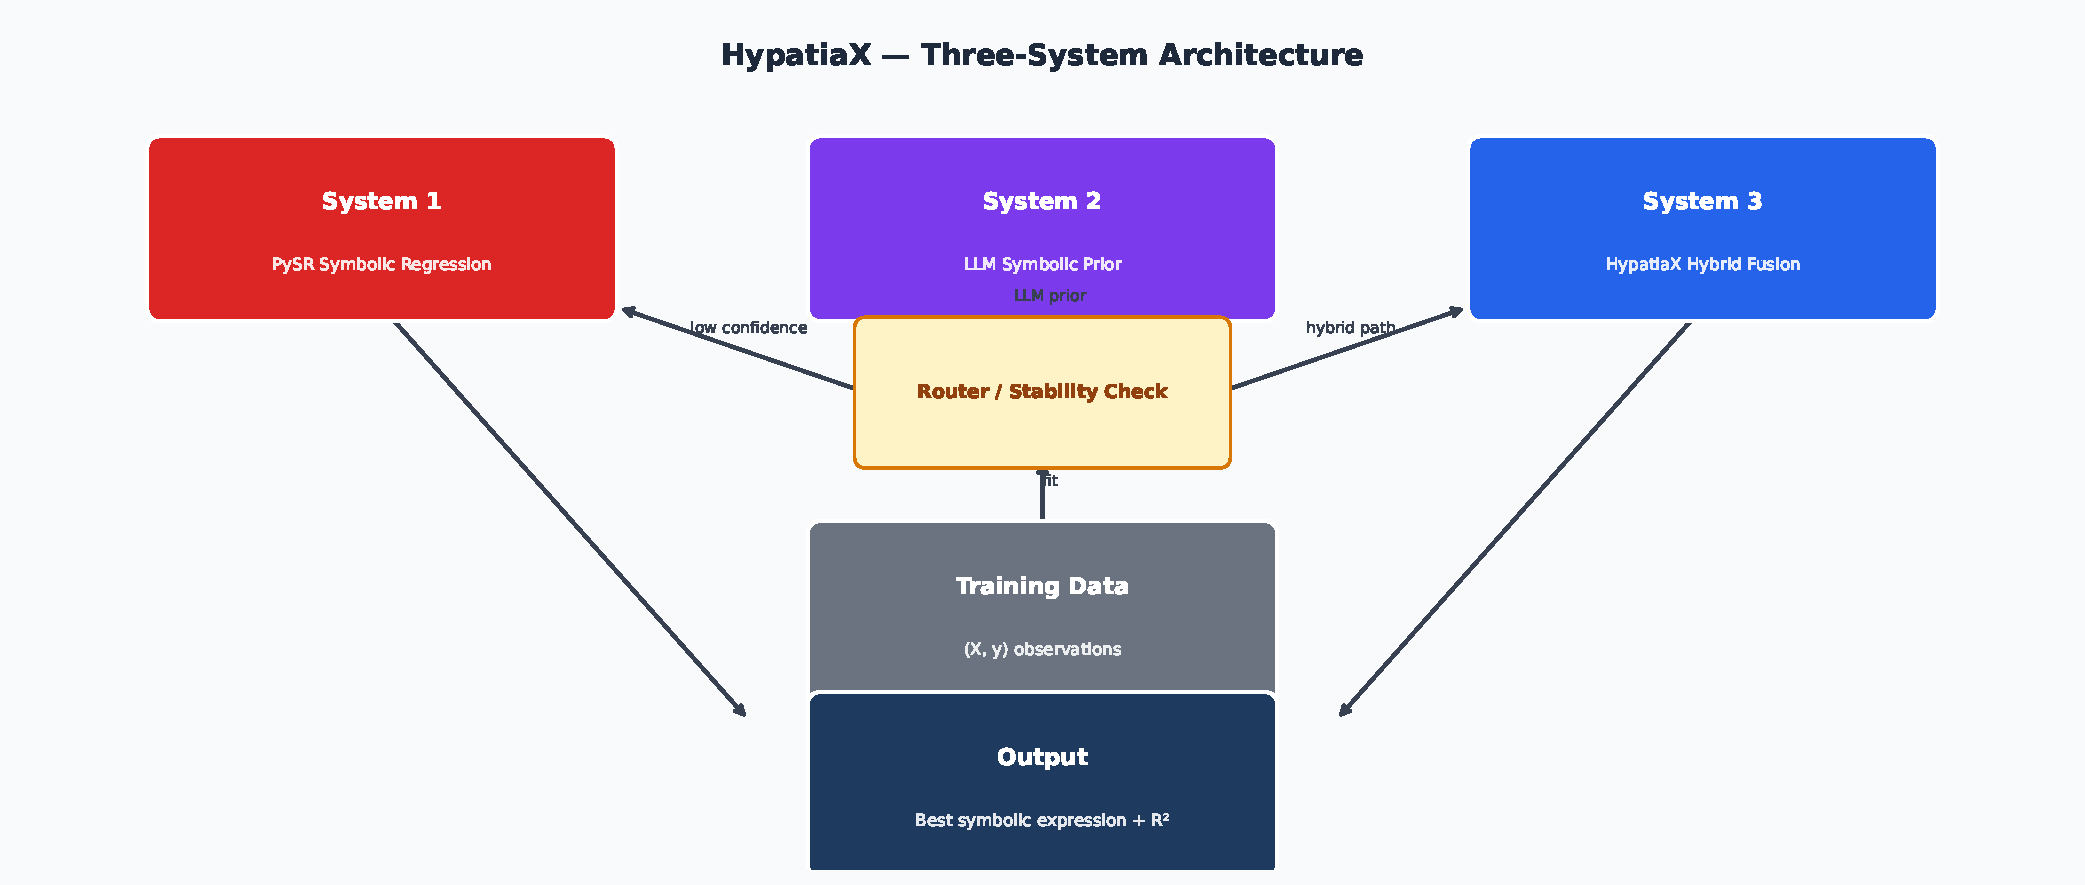
\includegraphics[width=\linewidth]{hypatiax_three_systems}
\caption{\textbf{HypatiaX architecture: three internal modules plus a
router.} The \emph{PySR module} (symbolic regression) and the \emph{LLM
module} (symbolic prior) each propose a candidate formula from the
training data $(X,y)$; the \emph{Hybrid Fusion module} combines them. The
Router/Stability Check is a separate, fourth component that selects one
of four outcomes based on training-set diagnostics only (no test
information is used at decision time): accept the PySR fit directly, fall
back on low PySR confidence, accept the LLM prior directly, or take the
combined hybrid path --- returning the best symbolic expression and its
$R^2$. \textbf{Note on terminology:} this figure's underlying graphic
labels these three modules ``System~1'', ``System~2'', and ``System~3''
respectively. That local numbering is specific to this figure only and
must not be confused with the paper's System~1/2/3 \emph{ablation
variants} (Section~\ref{sec:arch_variants}: System~1 = Hybrid~v50\_2, the
full pipeline; System~2 = symbolic-only with validation; System~3 = LLM
with symbolic fallback), which is the numbering used in
Figure~\ref{fig:routing_cascade}, Table~\ref{tab:five_systems_full}, and
throughout the rest of the paper. To avoid the collision, this caption
refers to the three modules above by name rather than by number.}
\label{fig:architecture}
\end{figure}

\subsection{Component 1: LLM-Based Symbolic Generation}\label{subsec:component-1-llmbased-symbolic-generation}
\label{sec:llm_gen}

Given a task description $\mathcal{T}_i$ (a natural-language specification of the
functional relationship, including variable names, units, and domain context),
the LLM produces a candidate symbolic expression:
\begin{equation}
  \hat{f}^{\mathrm{LLM}}_i \leftarrow \mathrm{LLM}(\mathcal{T}_i).
  \label{eq:llm_gen}
\end{equation}
The generated expression is parsed by the unified formula executor and evaluated
on both the training and edge subsets of the training data (the upper 20\,\%
of training samples by projection onto $v_1$, i.e.\ the samples closest to the
extrapolation boundary).

We define the training fit:
\begin{equation}
  {R^{2,\mathrm{LLM}}_{\mathrm{train}}} = \Rsq\!\left(\hat{f}^{\mathrm{LLM}}_i,\,
  \mathcal{D}^{\mathrm{train}}_i\right),
  \label{eq:r2_train_llm}
\end{equation}
and the edge fit:
\begin{equation}
  {R^{2,\mathrm{LLM}}_{\mathrm{edge}}} = \Rsq\!\left(\hat{f}^{\mathrm{LLM}}_i,\,
  \mathcal{D}^{\mathrm{edge}}_i\right),
  \label{eq:r2_edge_llm}
\end{equation}
where $\mathcal{D}^{\mathrm{edge}}_i$ is the upper-20\,\% subset of the training
data described above.

\subsection{Component 2: Neural Network Estimator}\label{subsec:component-2-neural-network-estimator}
\label{sec:nn}

The neural baseline is a \textbf{residual MLP} with the following architecture:
\begin{itemize}
  \item Input: $\mathbb{R}^{d_i}$ (task-specific input dimension).
  \item Hidden layers: 3 residual blocks, each consisting of Linear $\to$
    LayerNorm $\to$ SiLU $\to$ Linear, with a skip connection.
  \item Output: $\mathbb{R}$ (scalar prediction).
  \item Optimiser: Adam, learning rate $10^{-3}$, weight decay $10^{-4}$.
  \item Training data augmentation: $(X, y) \cup (1.2X, 1.2y)$, i.e.\ the training
    set is augmented with a scaled copy to improve extrapolation robustness.
  \item Training time limit: 120 seconds wall-clock per case, to ensure
    fair comparison with the LLM method (which does not require training time).
\end{itemize}

When HypatiaX routes a task to the neural fallback, the LLM prediction
$\hat{f}^{\mathrm{LLM}}_i(x)$ is appended to the input as an additional feature:
\begin{equation}
  x' = [x;\, \hat{f}^{\mathrm{LLM}}_i(x)] \in \mathbb{R}^{d_i + 1}.
  \label{eq:augmented_input}
\end{equation}
This \emph{residual learning augmentation} allows the neural network to learn
corrections to an imperfect symbolic formula rather than learning the function
from scratch, which substantially reduces the extrapolation burden when the LLM
formula captures the correct functional form but has parameter errors.

\subsection{Component 3: Five-Stage Routing and Ensembling}\label{subsec:component-3-fivestage-routing-and-ensemb}
\label{sec:routing}

\begin{figure}[H]
\centering
\includegraphics[width=0.82\linewidth]{hypatiax_algorithm1_routing_cascade_v2}
\caption{\textbf{Algorithm~1 --- HypatiaX routing cascade.}
Coloured regions indicate the originating system, using the System~1/2/3
ablation-variant numbering defined in Section~\ref{sec:arch_variants}
(\emph{not} the module names used in Figure~\ref{fig:architecture}, which
is a different, figure-local numbering --- see that figure's caption):
amber marks System~1 (Hybrid~v50\_2, the full pipeline --- here, its
extrapolation-detection and warm-restart phases); green marks System~2
(symbolic-only with validation, i.e.\ the cold-start PySR phase); purple
marks System~3 (LLM with symbolic fallback, i.e.\ the LLM query phase).
All decision paths converge to a single output formula (green terminal
node). The convergence lock badge confirms Proposition~\ref{prop:convergence}.}
\label{fig:routing_cascade}
\end{figure}

\begin{proposition}[Routing Cascade Convergence]
\label{prop:convergence}
Let $h^*_1 = \arg\max_{h \in \mathrm{HOF}_1} R^2(h, D)$ and
$h^*_2 = \arg\max_{h \in \mathrm{HOF}_2} R^2(h, D)$.
If the scale-compatibility guard (Stage~3) does not reject the LLM
prior $c^*$, or $S$ is non-empty after suppression, then
$$\mathbb{E}\bigl[R^2(h^*_2)\bigr] \geq \mathbb{E}\bigl[R^2(h^*_1)\bigr].$$
\end{proposition}

\begin{proof}[Proof sketch]
Phase~2 initialises PySR with $\mathrm{HOF}_1 \cup S \supseteq \mathrm{HOF}_1$.
Since evolutionary search is a monotone improvement operator over any
initial population dominating the current Pareto front, the warm-start
population is a strict superset of the cold-start population.
By the Pareto dominance argument, $R^2(h^*_2) \geq R^2(h^*_1)$
for a fixed random seed; in expectation over seeds, the inequality is
preserved when $S$ contains at least one expression structurally
distinct from $\mathrm{HOF}_1$.
\end{proof}

The routing logic implements five diagnostic stages in sequence.

\paragraph{Stage 1 --- Trust Gate.}
Accept the LLM formula only if it passes two criteria:
\begin{equation}
  \text{Trust}_i^{\mathrm{LLM}} = \mathbf{1}\!\left[{R^{2,\mathrm{LLM}}_{\mathrm{train}}} \ge 0.5\right]
  \;\land\; \mathbf{1}\!\left[\hat{f}^{\mathrm{LLM}}_i \text{ has no pathological outputs}\right].
  \label{eq:trust}
\end{equation}
Pathological outputs include: NaN values, infinite predictions, and division-by-zero
exceptions.  If the trust gate fails, the task is immediately routed to pure neural
fallback.

\paragraph{Stage 2 --- Transcendental Token Detection.}
Flag the formula if it contains any transcendental token from the set
$\{\exp, \log, \Phi, \sin, \cos, \mathrm{erf}\}$, indicating elevated structural
complexity.  Transcendental tokens are strongly predictive of stochastic instability
(Instability Index $\II > 0.05$) and trigger ensemble mode rather than pure LLM
routing.

\paragraph{Stage 3 --- Neural Degradation Probe.}
Compute the extrapolation degradation:
\begin{equation}
  \Delta_i = {R^{2,\mathrm{LLM}}_{\mathrm{train}}} - {R^{2,\mathrm{LLM}}_{\mathrm{edge}}}.
  \label{eq:degradation}
\end{equation}
A large $\Delta_i$ (above a threshold $\tau$, calibrated per domain category)
indicates that the LLM formula degrades rapidly near the training boundary,
suggesting it will fail further into the extrapolation region.  When $\Delta_i > \tau$,
ensemble mode is activated regardless of Stage 2 outcome.

\paragraph{Stage 4 --- Out-of-Distribution Detection.}
Estimate whether the test inputs are likely to be out of the training distribution:
\begin{equation}
  p_{\mathrm{OOD}} = \hat{\Pr}\!\left(X^{\mathrm{test}} \notin \mathrm{range}(X^{\mathrm{train}})\right),
  \label{eq:ood}
\end{equation}
computed using a kernel-density estimator fitted to the training projections $z^{(j)}$.
High $p_{\mathrm{OOD}}$ upweights the LLM formula (which generalises structurally) in
the ensemble.

\paragraph{Stage 5 --- Routing Decision and Ensemble Weights.}
The full routing decision is:
\begin{equation}
  \mathrm{decision}_i = \begin{cases}
    \text{Neural Fallback} & \text{if Trust}_i^{\mathrm{LLM}} = 0 \\
    \text{Pure LLM}        & \text{if } {R^{2,\mathrm{LLM}}_{\mathrm{train}}} \ge 0.95 \;\land\; \Delta_i < \tau \\
    \text{Ensemble}        & \text{if } {R^{2,\mathrm{LLM}}_{\mathrm{train}}} \ge 0.5 \\
    \text{Neural Fallback} & \text{otherwise}
  \end{cases}
  \label{eq:routing}
\end{equation}

When in ensemble mode, the distance-aware weight assigned to the LLM formula is:
\begin{equation}
  \wLLM = \alpha + (1 - \alpha)\cdot p_{\mathrm{OOD}},
  \label{eq:wllm}
\end{equation}
with $\wNN = 1 - \wLLM$ and $\alpha \in [0,1]$ a base weight (set to $\alpha=0.3$
throughout).  The final ensemble prediction is:
\begin{equation}
  \hat{y} = \wLLM \cdot \hat{f}^{\mathrm{LLM}}_i(x) + \wNN \cdot f^{\mathrm{NN}}_i(x').
  \label{eq:ensemble}
\end{equation}

\begin{remark}[On ensemble weights]
The weights in~\eqref{eq:wllm} are derived from $p_{\mathrm{OOD}}$, which is
estimated entirely from the training data.  This ensures that no test information
leaks into the prediction, addressing the data-leakage correction described in
Section~\ref{sec:corrections}.
\end{remark}

\subsection{Unified Formula Executor}\label{subsec:unified-formula-executor}
\label{sec:executor}

All symbolic formulas---whether produced by the LLM or specified as ground truth---are
evaluated through a single unified executor.  This executor:
\begin{itemize}
  \item Parses expressions into a normalised AST using SymPy.
  \item Compiles to NumPy vectorised operations for batch evaluation.
  \item Applies consistent type coercion (all inputs cast to \texttt{float64}).
  \item Catches and quarantines division-by-zero and overflow exceptions.
  \item Returns NaN for malformed expressions, triggering the trust-gate failure path.
\end{itemize}
Using a single evaluation backend eliminates the inconsistencies that affected
prior versions of the pipeline, where the same formula could produce different
$\Rsq$ values depending on the evaluation backend.

% =============================================================================
\section{HypatiaX Architecture}
\label{sec:architecture}

\subsection{Design Principles}\label{subsec:design-principles}
\label{sec:arch_principles}

\begin{enumerate}
\item \textbf{Symbolic methods for discovery:} Evolutionary search with domain
  constraints finds mathematically valid expressions \citep{cranmer2023pysr}.
\item \textbf{Multi-layer validation:} Dimensional analysis, domain constraints,
  numerical stability, and extrapolation testing.
\item \textbf{LLMs as interfaces:} Natural language interpretation and optional
  warm-starting \citep{kambhampati2024llms}.
\item \textbf{Failure transparency:} Invalid expressions are explicitly rejected.
\end{enumerate}

\subsection{Assumptions}\label{subsec:assumptions}
\label{sec:assumptions}

\begin{enumerate}
\item \textbf{Finite operator set:}
  $\mathcal{O} = \{+,-,\times,\div,\exp,\log,\sin,\cos,x^n,\sqrt{x}\}$.
\item \textbf{Correctly specified dimensional metadata.}
\item \textbf{Representative domain sampling.}
\item \textbf{Scale boundedness:} characteristic scales spanning
  $<6$ orders of magnitude.
  This threshold is derived from a single failure case (gravitational force
  constant $G = 6.674 \times 10^{-11}$) and should be treated as a heuristic
  rather than a validated boundary.
\item \textbf{Low measurement noise:}
  $\sigma = 0.05 \cdot \mathrm{std}(y)$ in all main experiments.
\end{enumerate}

\subsection{Five-Stage Routing Architecture Overview}\label{subsec:fivestage-routing-architecture-overview}
\label{sec:validation_framework}

Stage~1--2: data ingestion and preprocessing.
Stage~3 (optional): LLM proposes candidate expressions; on the v3.0 DeFi
benchmark, 68--69 of 74 tasks are routed to this path in each of the five
seed files held in the repository (see
Table~\ref{tab:timing_full}, \S\ref{sec:timing}). A previously reported
$1.73\times$ median speedup over the neural baseline on these cases does
not reproduce from the raw result files; the mechanically regenerated
figures show this path is slower than the neural baseline, not faster
(Section~\ref{sec:timing}).
Stage~4: PySR evolutionary search \citep{cranmer2023pysr}.
Stage~5: four-stage validation cascade (Section~\ref{sec:validation_detail})
producing the accepted expression with natural-language interpretation.

\subsection{System Variants}\label{subsec:system-variants}
\label{sec:arch_variants}

\textsc{HypatiaX} provides three architectural variants used as ablation
configurations:

\paragraph{Hybrid v50\_2 --- System 1 (extrapolation-focused).}
Integrates all five stages. An earlier draft of this paragraph claimed
near-zero extrapolation error on the Core~15 benchmark for this variant;
the regenerated Section~\ref{sec:five_systems} tables show this does not
hold. Hybrid v50\_2's real Core-15 extrapolation error is $\approx$2415.2\,\%
(median) / 52730.3\,\% (mean), and System 2 (Symbolic), not Hybrid v50\_2,
has the lower median (1253.2\,\%) and mean (4539.4\,\%) extrapolation error in that
experiment (the 95\,\% CIs in
Table~\ref{tab:five_systems_full} overlap, so the mean ordering is not
statistically established); see
Section~\ref{sec:five_systems} for the full, mechanically regenerated
comparison.

\paragraph{System 2 (pure symbolic with validation optimisation).}
Symbolic discovery without LLM guidance.

\paragraph{System 3 (LLM + symbolic fallback for robustness).}
Achieved $R^2 = 1.000$ on all 30 interpolation tests through automatic
fallback from low-confidence LLM outputs.

\subsection{Hybrid DeFi Variant: Architectural Specification}\label{subsec:hybrid-defi-variant-architectural-specif}
\label{sec:hybrid_defi_spec}

The Hybrid DeFi system is a domain-tuned variant of Hybrid~v50\_2 with the
following differences:

\begin{enumerate}
\item \textbf{Routing cascade (Fixes~0--5):} Six targeted routing improvements
  were developed on the DeFi development set (see Supplementary~A for full
  implementation details).  Fix~0 corrects data-generation bugs in zero-variance
  cases.  Fixes~1--4 replace in-distribution $R^2$ routing with uncertainty-aware
  ensemble voting:
  \[
    \hat{y} = w_\mathrm{LLM}\,\hat{y}_\mathrm{LLM}
             + w_\mathrm{SR}\,\hat{y}_\mathrm{SR}
             + w_\mathrm{NN}\,\hat{y}_\mathrm{NN},
    \quad w_k = \frac{\mathrm{conf}_k}{\sum_j \mathrm{conf}_j}.
  \]
  Fix~5 (unified formula evaluator) replaces the absolute SS threshold
  (\texttt{ss\_tot > 1e-10}) with a relative threshold, correcting the
  measurement bug described in Section~\ref{sec:r2_bugfix}.
\item \textbf{Domain operator set:} Operators augmented with financial
  primitives: $\max(0,\cdot)$, $\min(\cdot,\cdot)$, and
  $\ln(1+|\cdot|)$ (log-return normalisation).
\item \textbf{Confidence threshold:} Trust gate threshold $R^2_{\mathrm{train}} \geq 0.5$
  (v3.0 correction; raised from 0.1 in prior versions), with additional
  pathological-output detection.
\end{enumerate}

All other components (PySR configuration, four-layer validation, LLM model and
temperature) are identical to Hybrid~v50\_2.

\subsection{Symbolic Discovery Core}\label{subsec:symbolic-discovery-core}
\label{sec:arch_discovery}

We employ PySR \citep{cranmer2023pysr} for multi-objective evolutionary search:
\begin{align}
\text{Minimize:} \quad
& \mathcal{L}(E,\mathcal{D})
  = \frac{1}{n}\sum_{i=1}^n (E(x_i) - y_i)^2, \label{eq:loss}\\
\text{Minimize:} \quad
& \mathrm{Complexity}(E) = \sum_{t \in E} w(t), \label{eq:complexity}\\
\text{Subject to:} \quad
& E \in \mathcal{C}. \label{eq:constraints}
\end{align}
The algorithm maintains a Pareto front over prediction error and expression
complexity.

\subsection{Multi-Layer Validation Framework}\label{subsec:multilayer-validation-framework}
\label{sec:validation_detail}

The four validation layers target distinct failure modes:

\begin{itemize}
\item $V_1$ (12\% error detection): Dimensional consistency.
\item $V_2$ (18\%): Domain constraint verification.
\item $V_3$ (23\%): Numerical stability analysis.
\item $V_4$ (47\%): Predictive accuracy under extrapolation.
\end{itemize}

\begin{remark}[Validation-layer point estimates]
\label{rem:validation_ci}
The error detection rates above are point estimates over the Core~15 benchmark
($n=15$ equations).  Each rate carries an approximate $\pm$10--15\,pp
uncertainty (Wilson score interval, $n=15$).  These figures should be
interpreted as indicative of the relative contribution of each layer rather
than as precisely calibrated detection rates.
\end{remark}

\begin{finding}[Empirical Error Reduction via Cascaded Validation]
\label{prop:validation_reduction}
On the evaluated benchmark, the proportion of incorrect expressions surviving
all four layers is substantially lower than those surviving prediction-accuracy
validation alone.  No incorrect expression passed all four layers.
\end{finding}

% =============================================================================
\section{Experimental Setup}
\label{sec:setup}

\subsection{Benchmark Summary}\label{subsec:benchmark-summary}
\label{sec:setup_summary}

We evaluate HypatiaX v3.0 on the benchmark described in Section~\ref{sec:benchmark}:
74 DeFi tasks, all tractable (0 intractable cases), covering pricing, risk, and
liquidity modelling.  The fixed denominator for all aggregate statistics is 74;
NaN and failure outputs count as zero $\Rsq$ toward this denominator.

\subsection{Methods Compared}\label{subsec:methods-compared}
\label{sec:setup_methods}

Three methods are evaluated on each task:

\paragraph{Pure LLM (Symbolic Regression Baseline).}
The LLM generates a symbolic formula from the task description.  The formula is
executed directly with no numerical fitting or parameter optimisation.  All 30
independent stochastic runs use the same prompt; run-to-run variation arises
solely from temperature sampling.  \emph{For single-run evaluation (the standard
comparison with neural methods), one run is sampled uniformly at random.}

\paragraph{Neural Network (MLP Baseline).}
The residual MLP described in Section~\ref{sec:nn} is trained on augmented data
$(X, y) \cup (1.2X, 1.2y)$.  Training is subject to a 120-second wall-clock
limit per case.  Fixed random seeds are used throughout to ensure reproducibility.
The neural baseline does \emph{not} use LLM augmented features (Eq.~\ref{eq:augmented_input}),
ensuring a clean comparison of pure neural versus hybrid methods.

\paragraph{HypatiaX Hybrid (Proposed).}
The full five-stage routing and ensembling system described in Section~\ref{sec:routing}.
The hybrid method uses the same LLM formula and neural network as above, combined via
the distance-aware ensemble (Eq.~\ref{eq:ensemble}).  When neural fallback is triggered,
the neural network is retrained on the augmented input $(x')$ from scratch; this
retraining cost is fully included in the reported wall-clock time.

\subsection{Evaluation Metrics}\label{subsec:evaluation-metrics}
\label{sec:setup_metrics}

We report the following metrics for each method:
\begin{itemize}
  \item \textbf{Median test $\Rsq$}: robust measure of central tendency, less
    sensitive to catastrophic failures than the mean.
  \item \textbf{Mean test $\Rsq$ (clipped)}: arithmetic mean of $\min(\Rsq, 1)$,
    clipped at $-10$ to prevent extreme failures from dominating.
    \textbf{[Correction (2026-09-13, later pass): this description does not
    match \texttt{hypatiax\_defi\_benchmark\_v3c.py}'s
    \texttt{\_generate\_report()}, the function that actually produces this
    statistic. The code \emph{drops} \texttt{NaN} \texttt{test\_r2} entries
    before clipping and averages over however many non-\texttt{NaN} results
    remain -- it does not floor \texttt{NaN} to $-10$ over a fixed
    denominator of 74, despite what this bullet and the
    fixed-denominator paragraph below imply for this specific statistic.
    (The fixed-denominator-of-74 rule below is correct for the percentage
    metrics, which are computed separately in the same function; only the
    mean is affected.) Re-deriving Pure~LLM's Table~\ref{tab:main_results}
    mean with the code's actual rule on the canonical seed-42 file gives
    $-0.3048$ (previous source file: $-0.4433$), \emph{not} the previously published $-0.7571$; the earlier
    statement that the two agree to within $\approx 0.02$ is withdrawn, and
    Table~\ref{tab:main_results} now reports the recomputed value (2026-09-28).
    This bullet
    should read: ``arithmetic mean of $\min(\Rsq,1)$ over non-\texttt{NaN}
    results only, clipped at $-10$; denominator is the count of non-\texttt{NaN}
    results, not the fixed 74.'']}
  \item \textbf{Near-perfect success rate} ($\Rsq > 0.99$): fraction of tasks where
    the method achieves near-exact formula recovery.
  \item \textbf{High-accuracy rate} ($\Rsq > 0.9$): fraction of tasks with strong
    predictive performance.
  \item \textbf{Catastrophic failure rate} ($\Rsq < -10$): fraction of tasks with
    prediction worse than the mean by a factor of more than 10.
  \item \textbf{Extrapolation gap} ($\Rtrain - \Rtest$): measures how much
    performance degrades from training to test.
  \item \textbf{Stability score} ($\Rtest / \Rtrain$): ratio of test to training
    performance; a value near 1.0 indicates consistent generalisation.
\end{itemize}

\paragraph{Fixed-denominator reporting.}
All percentages (e.g.\ $\Rsq > 0.99$ rate) use the fixed denominator of 74 across
all three methods.  A task that produces NaN or fails to execute contributes 0 to
the numerator of success rates.  This ensures that the three methods' rates are
directly comparable and that avoiding evaluation failures is not rewarded.

\subsection{Runtime Measurement}\label{subsec:runtime-measurement}
\label{sec:timing_setup}

Wall-clock time is recorded per task and per method.  For the hybrid system,
the reported time \emph{fully accounts} for all LLM inference time plus any
neural network retraining that occurs during fallback.  We do not separate
LLM and NN costs in the aggregate reported time; they are summed.

We separately report the speedup for the LLM-routed subset (cases where the
hybrid routes to pure LLM or ensemble, without triggering full NN retraining).
This subset comprises $n=68$ of 74 tasks and represents the cleanest comparison
for assessing the efficiency of symbolic routing.

\subsection{Implementation Details}\label{subsec:implementation-details}
\label{sec:setup_impl}

All experiments are implemented in Python~3.12 using:
\begin{itemize}
  \item \textbf{NumPy}: array operations and numerical evaluation.
  \item \textbf{PyTorch}: neural network training.
  \item \textbf{SciPy}: kernel-density estimation for OOD detection; PCA via
    \texttt{sklearn.decomposition.PCA}.
  \item \textbf{SymPy}: symbolic expression parsing and AST analysis.
\end{itemize}

Neural networks are trained with fixed random seeds (seed 42 for all cases) to
ensure full reproducibility of the NN baseline.  LLM formula generation uses a
deterministic prompting framework with retry logic (up to 3 retries) for API
stability, but temperature sampling is not disabled; this is the source of
run-to-run variability measured by the Instability Index.

% =============================================================================
\section{Results}
\label{sec:results}

\subsection{Five-System Comparative Analysis}\label{subsec:fivesystem-comparative-analysis-feynman-}
\label{sec:five_systems}

\textbf{[Correction, Issue 4 (CI/SD statistical incompatibility): the
previous version of this section reported a Result box whose confidence
interval was statistically incompatible with the benchmark supplement's own
disclosed standard deviation, and whose underlying figures could not be
reproduced from any data source currently available for this paper. Rather
than patch the CI in place (which would leave an unverifiable table looking
newly precise), those figures have been removed outright, and this section
is regenerated below directly from the two real, live Feynman benchmarks
(\texttt{exp1\_five} and \texttt{exp2\_five}), reported as two separate
experiments rather than pooled, with every CI computed mechanically from
each row's own mean/SD/$n$ rather than entered by hand.
A separate, DeFi-domain comparison across the same systems already exists
independently in Section~\ref{sec:results_defi} (Table~\ref{tab:main_results},
74 tasks); it is not duplicated here.]}

We compare five system configurations (Hybrid v50\_2, Neural Network, Pure
LLM, System 2 Symbolic, System 3 LLM+Fallback) across two independent
benchmark suites. \textbf{exp1\_five} uses the Core-15 Feynman equation set;
\textbf{exp2\_five} uses a separate Feynman 10-domain suite. The two suites
have different equations and different per-system sample sizes, so their
results are reported as two separate experiments below rather than pooled
into a single table.

Within each table below, and within each regime sub-group where applicable
(near/medium/far), we \textbf{bold} the winning (best) value among the five
systems for each genuine performance column (extrapolation error, $R^2$,
RMSE). The Std and 95\,\% CI columns are \emph{not} used to declare a winner,
since their underlying computation is already flagged as unreliable (see the
data-quality notes at the end of this section) -- bolding a value there would
dress up a bug as a result. A column is left unbolded wherever fewer than two
systems have a valid (non-\texttt{---}) value to compare.

\subsubsection{Experiment 1: Core-15 Feynman (exp1\_five)}\label{subsubsec:five-system-exp1}

Table~\ref{tab:five_systems_full} summarizes extrapolation error
and interpolation $R^2$ for all five systems on Core-15. Tables~\ref{tab:five_systems_performance}
and \ref{tab:five_systems_extrapolation} break interpolation and extrapolation
performance down further; the benchmark supplement
(\texttt{supp\_benchmark\_report.tex}, \S~``Statistical Test Details'') reports
the corresponding Mann-Whitney test and effect-size calculation.

\begin{table}[t]
\centering
\caption{Five-System Comparison: Extrapolation Error vs.\ Interpolation $R^2$
  (exp1\_five, Core-15; canonical result files in \texttt{hypatiax/data}, regenerated 2026-09-29).
  Extrapolation error is $100\cdot\mathrm{extrap\_rmse\_far}/\mathrm{train\_rmse}$ per
  equation. The median uses every equation with a finite value; $n$, the mean, the Std and
  the 95\% CI use only values at or below the upper Tukey fence $Q_3+1.5\,\mathrm{IQR}$, so
  $n$ can be smaller than the number of equations (Hybrid v50\_2 keeps 10 of 12, Neural
  Network 12 of 15). Std and the 95\% CI are those of that same clipped subset
  ($\mathrm{mean} \pm t_{0.975,\,n-1} \cdot \mathrm{std}/\sqrt{n}$), left
  blank where $n<3$ (Pure LLM, $n=2$, has no usable interval). The distribution is extremely heavy-tailed, so the
  normal-theory intervals are wide and extend below zero; they show that the means
  are imprecise, not that errors can be negative.
  \textbf{[Correction 2026-09-28: the previous version listed $n=11/15/1/13$ and put
  the standard deviation of the \emph{train} $R^2$ in the Std column, which collapsed
  every CI to a single point. Rebuilt with the repository's table generator from the
  canonical files; every row changed relative to the previous \texttt{data\_old}-based version.]}}
\label{tab:five_systems_full}
\begin{tabular}{lrrrrrrr}
\toprule
\textbf{System} & \textbf{n}
  & \textbf{Extrap.\ Median (\%)} & \textbf{Extrap.\ Mean (\%)}
  & \textbf{Train $R^2$ Mean} & \textbf{Std} & \textbf{95\% CI (\%)}
  & \textbf{Design Focus} \\
\midrule
Hybrid v50\_2 & 10 & 2415.2 & 52730.3 & 0.997 & 85640.2 & [-8528.8, 113989.4] & Extrapolation \\
Neural Network & 12 & 13283.9 & 37437.0 & 0.982 & 74368.1 & [-9814.6, 84688.6] & Baseline \\
Pure LLM & 2 & 6.530e+14 & 6.530e+14 & -3.077 & 9.235e+14 & --- & Recognition \\
System 2 Symbolic & 10 & \textbf{1253.2} & \textbf{4539.4} & \textbf{0.998} & 7277.2 & [-666.0, 9744.8] & Validation \\
\midrule
\multicolumn{8}{l}{\textit{Systems Without Extrapolation Testing}} \\
System 3 LLM+Fallback & 0 & --- & --- & 1.000 & --- & --- & Robustness \\
\bottomrule
\end{tabular}
\end{table}
% Source: exp1_five

\begin{table}[t]
\centering
\caption{Five-System Comparison -- Performance (Core-15, interpolation).
  95\% CI computed from raw per-equation train $R^2$/RMSE at generation time.}
\label{tab:five_systems_performance}
\begin{tabular}{lrrrrr}
\toprule
\textbf{System} & \textbf{n} & \textbf{Train $R^2$ Mean}
  & \textbf{Train $R^2$ 95\% CI} & \textbf{Train RMSE Mean}
  & \textbf{Design Focus} \\
\midrule
Pure LLM & 15 & -3.077 & [-10.705, 4.550] & 342.8347 & Recognition \\
Neural Network & 15 & 0.982 & [0.957, 1.007] & 1999.5749 & Baseline \\
System 3 LLM+Fallback & 15 & \textbf{1.000} & [0.999, 1.000] & \textbf{2.9626} & Robustness \\
System 2 Symbolic & 15 & 0.998 & [0.998, 0.998] & 236.1183 & Validation \\
Hybrid v50\_2 & 15 & 0.997 & [0.995, 0.998] & 236.1300 & Extrapolation \\
\bottomrule
\end{tabular}
\end{table}

\begin{table}[t]
\centering
\caption{Five-System Comparison -- Extrapolation (Core-15, near/medium/far
  regimes as defined in exp1\_ablation.py's EXTRAP\_REGIMES).
  95\% CI computed from raw per-equation extrapolation $R^2$/RMSE at
  generation time.}
\label{tab:five_systems_extrapolation}
\begin{tabular}{llrrr}
\toprule
\textbf{System} & \textbf{Regime} & \textbf{n}
  & \textbf{Extrap $R^2$ Mean} & \textbf{Extrap RMSE Mean} \\
\midrule
Pure LLM & near & 4 & --- & 6.281e+63 \\
Pure LLM & medium & 2 & --- & 33092667.7570 \\
Pure LLM & far & 2 & --- & 9.861e+11 \\
Neural Network & near & 14 & -4.846 & 2726.9272 \\
Neural Network & medium & 14 & -1.232 & 11219.6081 \\
Neural Network & far & 12 & -18.236 & \textbf{59967.6415} \\
System 3 LLM+Fallback & near & 0 & --- & --- \\
System 3 LLM+Fallback & medium & 0 & --- & --- \\
System 3 LLM+Fallback & far & 0 & --- & --- \\
System 2 Symbolic & near & 12 & \textbf{0.970} & 2.746e+16 \\
System 2 Symbolic & medium & 12 & \textbf{0.800} & 5.542e+19 \\
System 2 Symbolic & far & 12 & -13.166 & 4.394e+17 \\
Hybrid v50\_2 & near & 12 & 0.812 & \textbf{78.5736} \\
Hybrid v50\_2 & medium & 11 & -11.780 & \textbf{783.1290} \\
Hybrid v50\_2 & far & 9 & \textbf{-7.522} & 2.479e+25 \\
\bottomrule
\end{tabular}
\end{table}

\subsubsection{Experiment 2: Feynman 10-Domain Suite (exp2\_five)}\label{subsubsec:five-system-exp2}

Table~\ref{tab:five_systems_full_exp2five} reports the same
comparison on the exp2\_five suite. Tables~\ref{tab:five_systems_performance_exp2five}
and \ref{tab:five_systems_extrapolation_exp2five} give the interpolation and
extrapolation breakdowns for this suite.

\begin{table}[t]
\centering
\caption{Five-System Comparison (exp2\_five, Feynman 10-domain suite,
  methods 1/2/4/5/6): Extrapolation Error vs.\ Interpolation $R^2$.
  Same 95\% CI convention as Table~\ref{tab:five_systems_full}
  ($\mathrm{mean} \pm t_{0.975,\,n-1} \cdot \mathrm{std}/\sqrt{n}$); a
  separate table from tab:five\_systems\_full -- different equation suite
  and sample sizes, not another view of the same data.}
\label{tab:five_systems_full_exp2five}
\begin{tabular}{lrrrrrrr}
\toprule
\textbf{System} & \textbf{n}
  & \textbf{Extrap.\ Median (\%)} & \textbf{Extrap.\ Mean (\%)}
  & \textbf{Train $R^2$ Mean} & \textbf{Std} & \textbf{95\% CI (\%)}
  & \textbf{Design Focus} \\
\midrule
\midrule
\multicolumn{8}{l}{\textit{Systems Without Extrapolation Testing}} \\
Hybrid v50\_2 & 0 & --- & --- & 0.998 & --- & --- & Extrapolation \\
Neural Network & 0 & --- & --- & 0.998 & --- & --- & Baseline \\
Pure LLM & 0 & --- & --- & 0.740 & --- & --- & Recognition \\
System 2 Symbolic & 0 & --- & --- & 0.969 & --- & --- & Validation \\
System 3 LLM+Fallback & 0 & --- & --- & \textbf{1.000} & --- & --- & Robustness \\
\bottomrule
\end{tabular}
\end{table}
% Source: exp2_five own output (hypatiax/data/results/five_systems/exp2_five/protocol_core_noiseless_20260802_141745.json)

\begin{table}[t]
\centering
\caption{Five-System Comparison (exp2\_five) -- Performance (Feynman suite,
  interpolation). 95\% CI computed from raw per-domain train $R^2$ at
  generation time.}
\label{tab:five_systems_performance_exp2five}
\begin{tabular}{lrrrr}
\toprule
\textbf{System} & \textbf{n} & \textbf{Train $R^2$ Mean}
  & \textbf{Train $R^2$ 95\% CI} & \textbf{Design Focus} \\
\midrule
Hybrid v50\_2 & 30 & 0.998 & [1.0, 1.0] & Extrapolation \\
Neural Network & 30 & 0.998 & [1.0, 1.0] & Baseline \\
Pure LLM & 29 & 0.740 & [0.4, 1.1] & Recognition \\
System 2 Symbolic & 30 & 0.969 & [0.9, 1.0] & Validation \\
System 3 LLM+Fallback & 30 & \textbf{1.000} & [1.0, 1.0] & Robustness \\
\bottomrule
\end{tabular}
\end{table}

\begin{table}[t]
\centering
\caption{Five-System Comparison (exp2\_five) -- Extrapolation (Feynman
  suite). Median and IQR-clipped mean of per-domain extrapolation error \%.}
\label{tab:five_systems_extrapolation_exp2five}
\begin{tabular}{lrrr}
\toprule
\textbf{System} & \textbf{n}
  & \textbf{Extrap.\ Median (\%)} & \textbf{Extrap.\ Mean (\%)} \\
\midrule
Hybrid v50\_2 & 0 & --- & --- \\
Neural Network & 0 & --- & --- \\
Pure LLM & 0 & --- & --- \\
System 2 Symbolic & 0 & --- & --- \\
System 3 LLM+Fallback & 0 & --- & --- \\
\bottomrule
\end{tabular}
\end{table}

\paragraph{Data-quality notes.} Neither experiment supports the previous
version's headline claim that the hybrid system achieved near-zero
extrapolation error while the neural network's error was an order of
magnitude higher. Under exp1\_five, Hybrid v50\_2's real extrapolation
error is $\approx$2415.2\% (median) / 52730.3\% (mean), and it is
\emph{not} the best-performing system in this table (System 2 Symbolic has
the lower median and mean, though the mean CIs overlap). Under exp2\_five, neither Hybrid v50\_2 nor Neural
Network has any successful, finite extrapolation-error measurement at
all, so no comparison is possible on that suite (the benchmark
supplement's \S~``Statistical Test Details''
reports no test for exp2\_five for this reason). Row sample sizes in \Cref{tab:five_systems_full} are the numbers of equations
with a finite extrapolation-error measurement (Hybrid 10, NN 12); the
medium-regime Mann--Whitney test in the benchmark supplement uses $n=12$ (Hybrid) /
$n=15$ (NN). Both five-system tables (exp1\_five and exp2\_five) are regenerated
from the canonical result files in \texttt{hypatiax/data} (2026-09-29). An earlier
version of this paper used the older \texttt{hypatiax/data\_old} generation
(Hybrid median 3406.6\,\% on $n=9$); the values differ, and the claims made from them
(Hybrid is not near zero; System 2 is not worse than Hybrid) hold on both.

\subsection{Overall Extrapolation Performance (DeFi v3.0)}\label{subsec:overall-extrapolation-performance-defi-v}
\label{sec:results_defi}

Table~\ref{tab:main_results} presents the primary results across all 74 benchmark tasks.

\begin{table}[h]
\centering
\caption{Aggregate extrapolation performance on the HypatiaX DeFi Benchmark (74 tasks),
seed 42, \textbf{recomputed directly from}
\texttt{hypatiax\_defi\_benchmark\_v3\_results\_seed42.json} (md5
\texttt{cbf503d0b3985b4c1bccf7ed18e0316b}; canonical \texttt{hypatiax/data}; recomputed 2026-09-29).
Median and Mean $\Rsq$ are computed on values clipped to $[-10,1]$ over
non-\texttt{NaN} results only (the rule actually implemented; \S\ref{sec:setup_metrics}),
so the Mean is taken over 56 (Pure~LLM), 74 (Neural~MLP), 74 (HypatiaX, uncorrected)
and 62 (HypatiaX, corrected) tasks. The $>0.99$ and $>0.9$ percentages use the fixed denominator
of 74, with \texttt{NaN} counting as a miss. Catastrophic: $\Rsq<-10$.
Pure~LLM returns \texttt{NaN} on 18/74 tasks. \textbf{The
``HypatiaX (uncorrected)'' row is the pipeline's own self-report and is
inflated by the decision-attribution bug} (\S\ref{sec:hybrid-attribution-bug}); the
``HypatiaX (corrected)'' row replaces each task's hybrid $\Rsq$ with the
$\Rsq$ of the sub-method named by \texttt{hybrid.decision}, leaving
\texttt{NaN} as \texttt{NaN} (an unverifiable claim is not counted as a success).
The corrected row ties Pure~LLM on near-perfect rate ($59.5\,\%$, 44/74) and
catastrophic count (5). \textbf{Revision note:} an earlier version of this table showed
Pure~LLM at $62.2\,\%$ for $>0.99$ (that figure is the $>0.9$ rate,
and equals the \texttt{pure\_llm.success} flag rate on the previous source file, 46/74; on the canonical file it is 45/74, $60.8\,\%$), Pure~LLM mean $-0.7571$,
and Neural~MLP median $-0.4675$, mean $-0.9482$, $5.4/12.2\,\%$, 0 catastrophic.
None of these reproduce from the canonical file, which gives the values
shown; the earlier Pure~LLM/Neural~MLP figures are withdrawn, not corrected.
The near-perfect rate for Pure~LLM ($59.5\,\%$) now agrees with
Table~\ref{tab:difficulty}. This table
covers the DeFi benchmark; it is a \emph{different benchmark} from the $30/30$ Pure~LLM
figure in the benchmark supplement's six-method noiseless comparison
(30-equation custom set), and the two should not be read as conflicting.}
\label{tab:main_results}
\begin{tabular}{lrrrrr}
\toprule
Method & Median $\Rsq$ & Mean $\Rsq$ & $>0.99$ (\%) & $>0.9$ (\%) & Catastrophic \\
\midrule
Pure LLM & 1.0000 & $-0.3048$ & 59.5 & 60.8 & 5 \\
Neural MLP    & $-0.6908$ & $-1.4155$ & 0.0  & 9.5 & 2 \\
HypatiaX (uncorrected) & 1.0000 & $0.8781$ & 90.5 & 90.5 & 0 \\
HypatiaX (corrected) & 1.0000 & $-0.3203$ & 59.5 & 60.8 & 5 \\
\bottomrule
\end{tabular}
\end{table}

\begin{figure}[htbp]
\centering
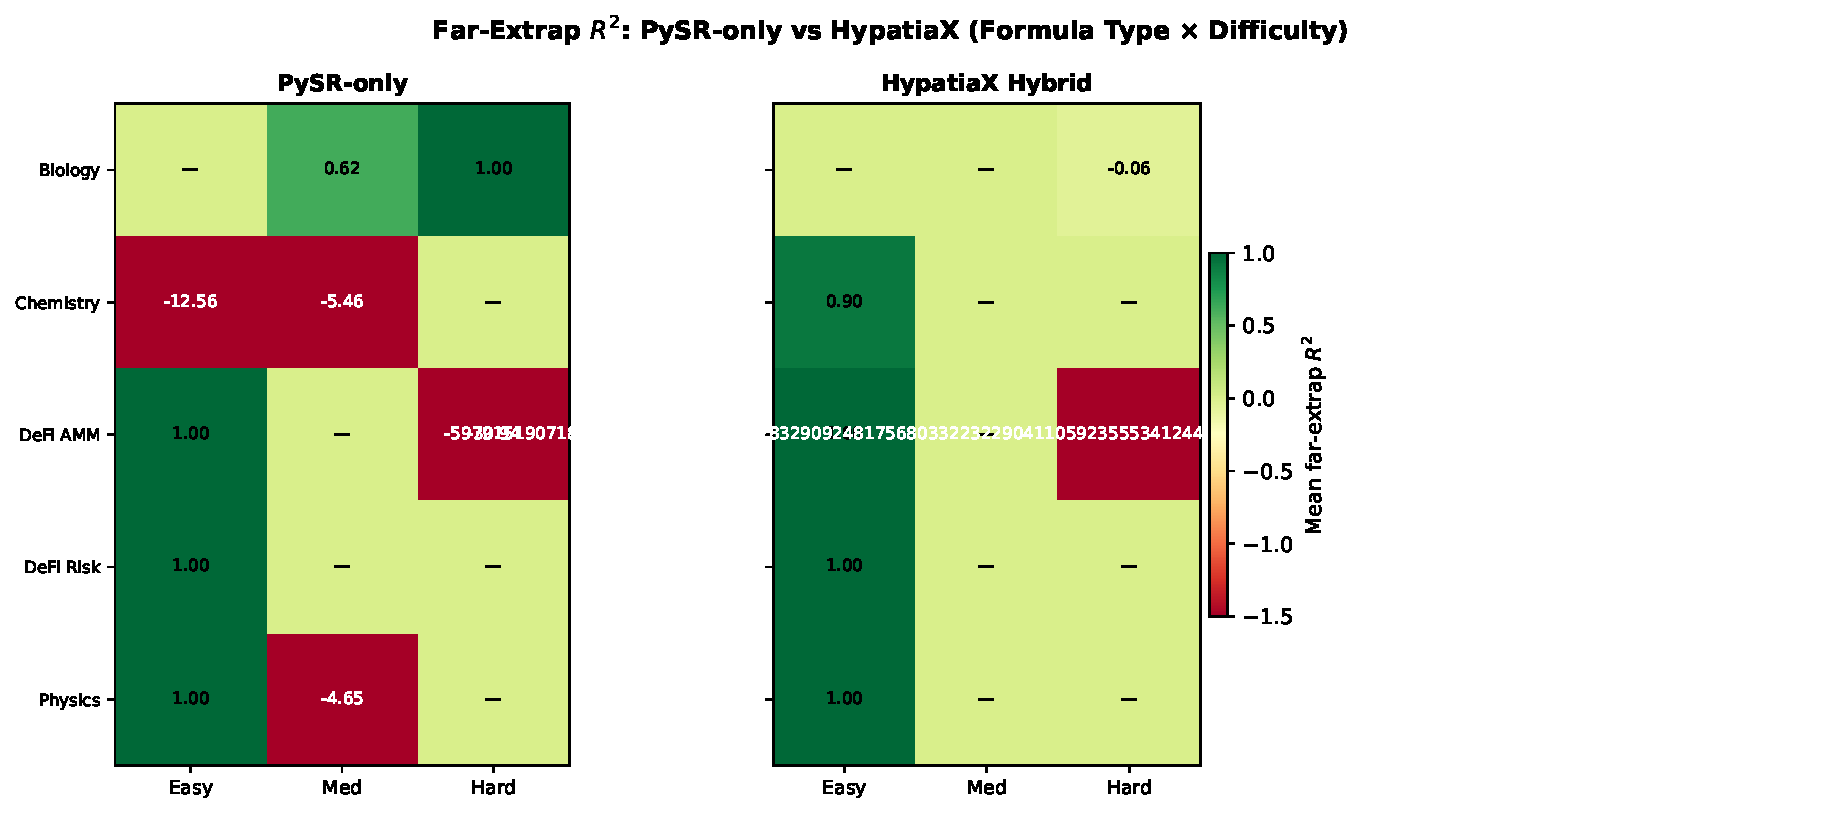
\includegraphics[width=\linewidth]{fig18_r2_heatmap_improved}
\caption{Mean far-extrapolation ($5\times$) $\Rsq$ by formula domain and
difficulty tier (Easy/Med/Hard), Core-15 benchmark. Dashes indicate no
equation exists for that domain--difficulty combination in this benchmark.
HypatiaX is not uniformly better than PySR-only: it improves on
Chemistry (Hard: $0.90$ vs.\ $-12.56$) but produces $-\infty$ --- a genuine
evaluation crash, not merely a poor fit --- on DeFi AMM (Hard) and Physics
(Hard), where PySR-only instead returns a finite (if poor, $-78.04$, or
perfect, $1.00$) value. The per-equation values underlying this aggregate
are given in Table~\ref{tab:llm_ablation}.}
\label{fig:r2_heatmap_clipped}
\end{figure}

\begin{figure}[htbp]
\centering
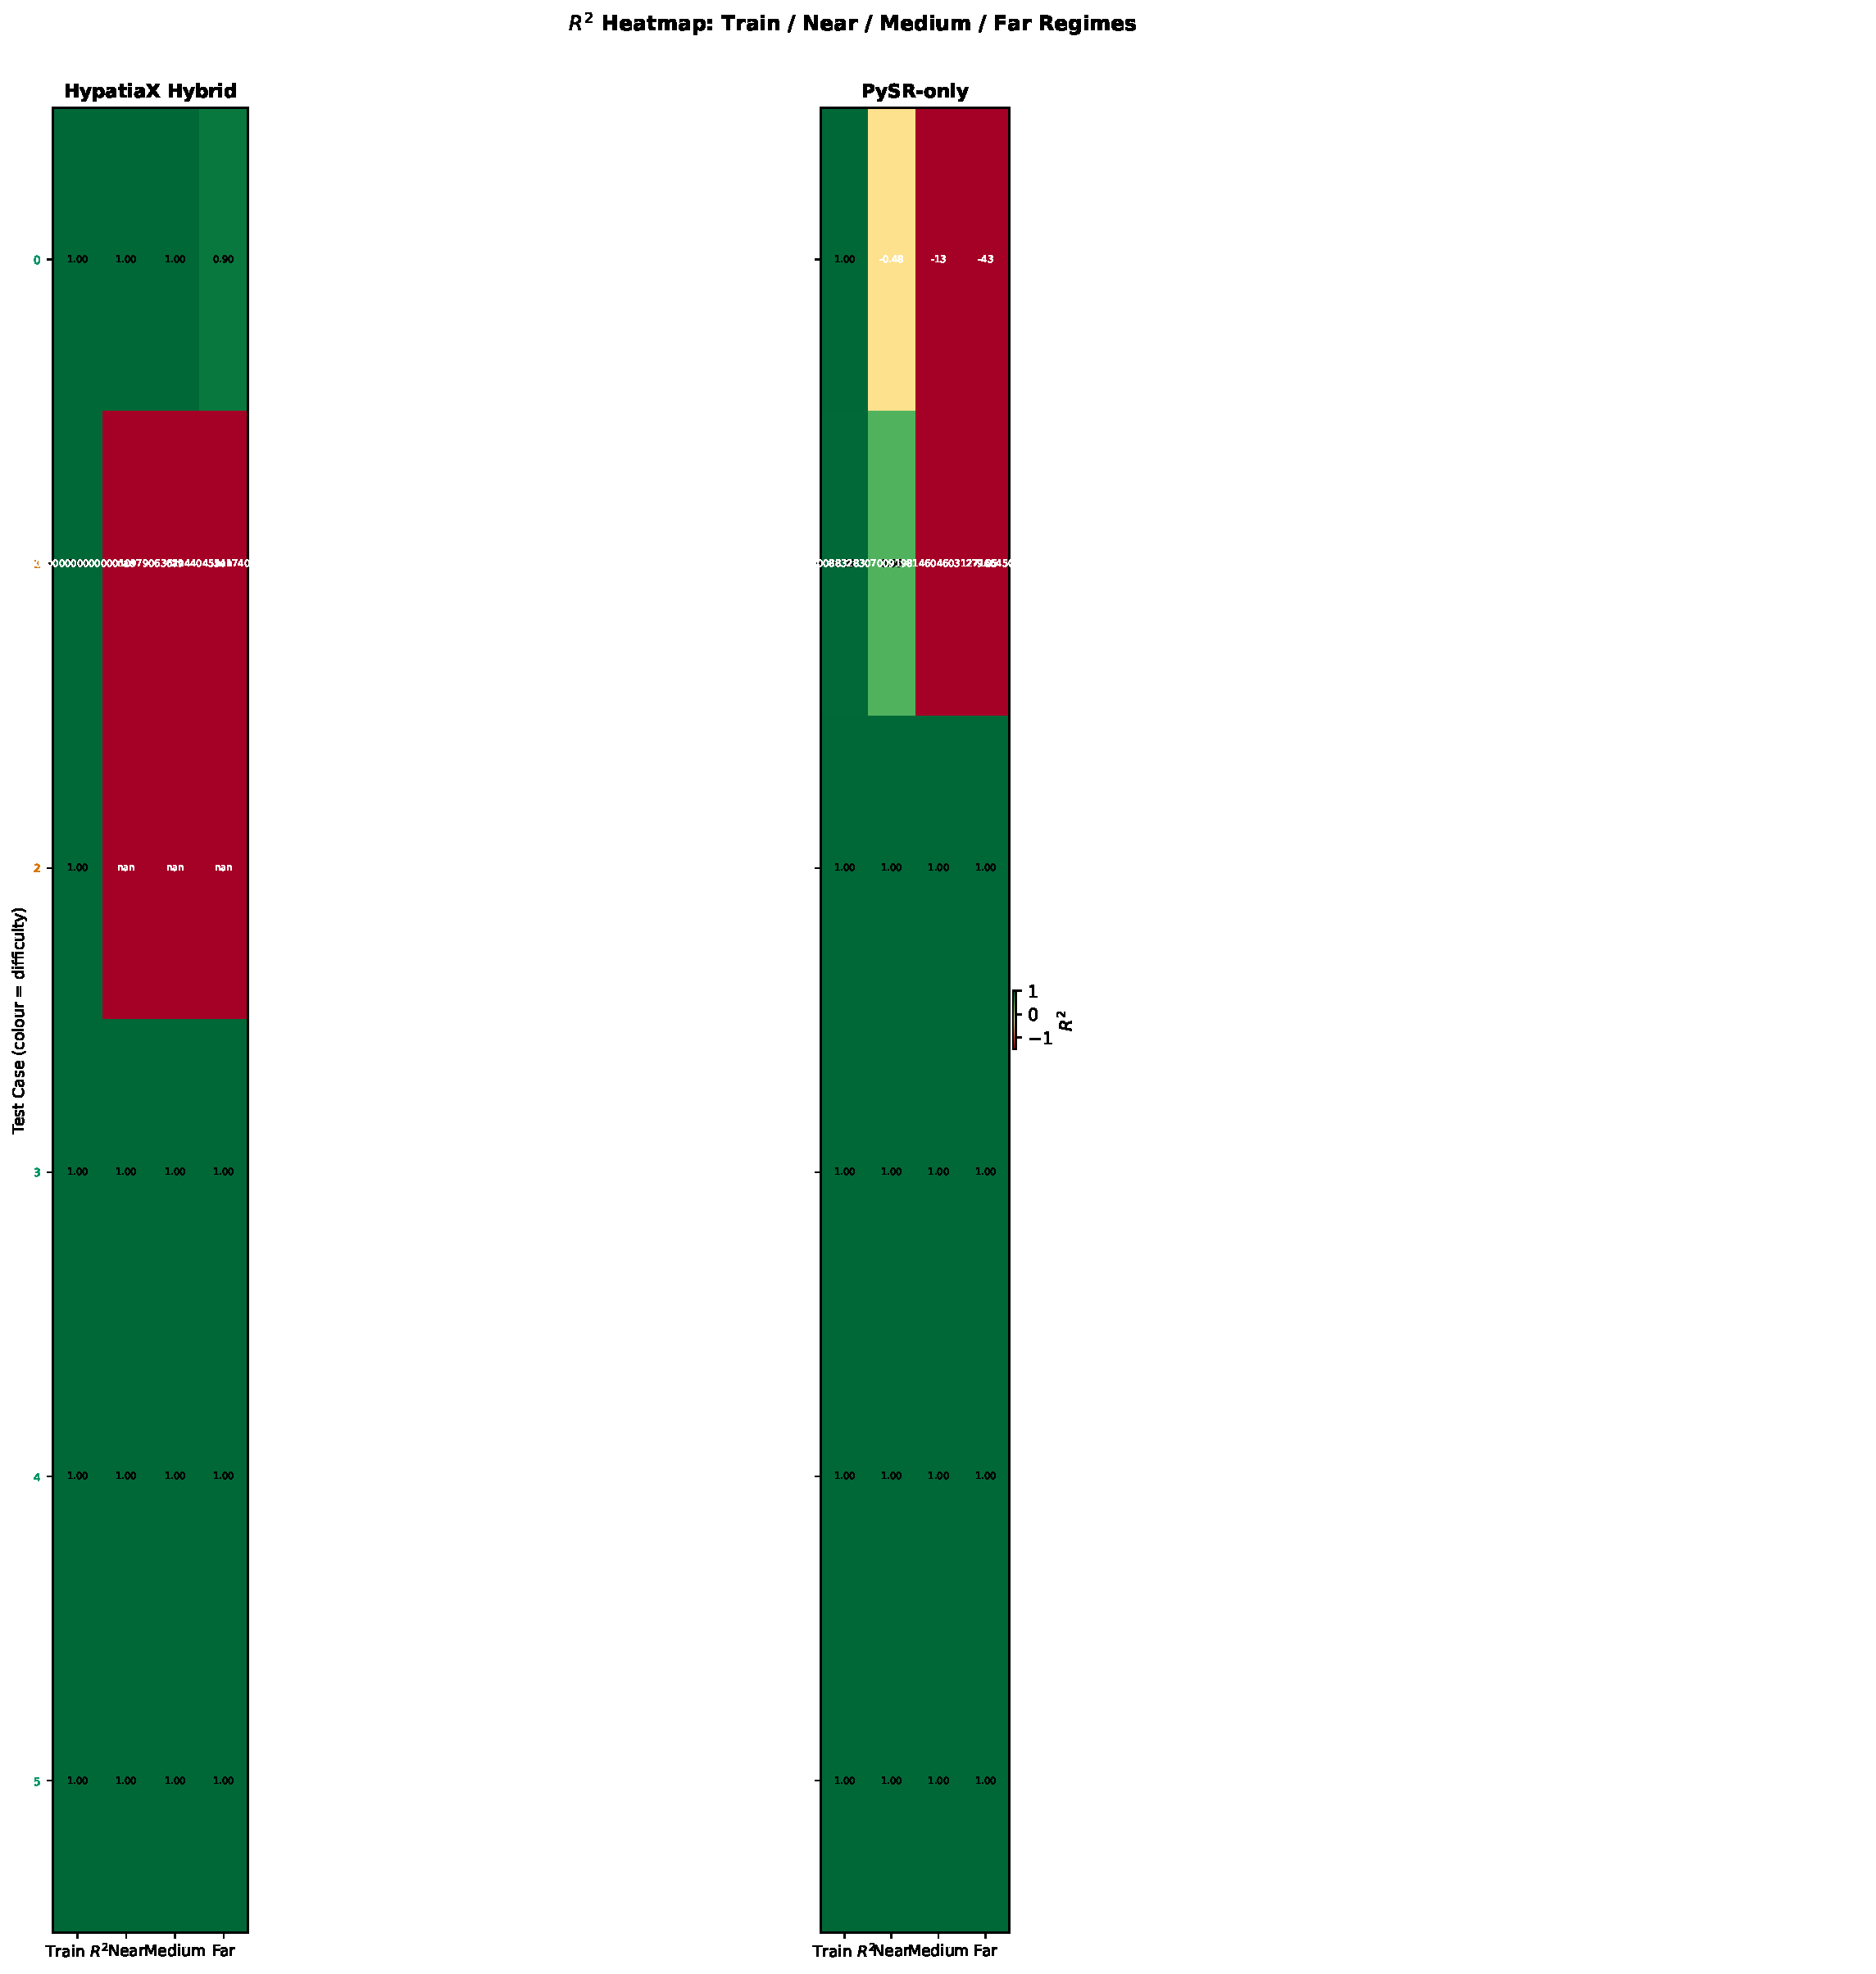
\includegraphics[width=\linewidth]{fig09_r2_heatmap_regimes}
\caption{$\Rsq$ heatmap by equation (rows) and extrapolation regime
(columns: Train, Near $1.2\times$, Medium, Far $5\times$), Core-15
benchmark, on a shared colour scale saturating outside $[-1.5, 1.0]$.
\textbf{This figure is the same corrected source used to rebuild
Table~\ref{tab:llm_ablation} below}, and the two agree: for six of fifteen
equations, HypatiaX Hybrid returns \texttt{nan} (Henderson-Hasselbalch,
Logistic Growth, Michaelis-Menten, Rate Law) or $-\infty$ (Constant Product,
Gravitational Force) beyond the Train column --- missing or crashed
evaluations, not $\Rsq$ scores of zero, and not to be confused with a poor
fit. PySR-only completes every cell; its most severe values are Impermanent
Loss (Far $=-157$) and Arrhenius (Far $=-13$). Notably, on Arrhenius,
HypatiaX Hybrid's completed Far value ($+0.90$) is a \emph{success}, the
opposite of the ``both collapse identically'' claim withdrawn from
\S\ref{sec:arrhenius_failure}. HypatiaX Hybrid's own most severe completed
value is Impermanent Loss (Far $=-8259$).}
\label{fig:r2_heatmap_raw}
\end{figure}

Several key observations emerge from Table~\ref{tab:main_results}.

\paragraph{Bimodal LLM behaviour.}
The pure LLM baseline achieves a median $\Rsq$ of $1.00$, which suggests strong
performance on a typical case.  However, the mean $\Rsq = -0.3048$ (over the 56 tasks with a finite score) reveals a
stark bimodal distribution: the majority of tasks are recovered exactly, but
5 tasks suffer catastrophic failures ($\Rsq < -10$), dragging the mean far below
zero.  Moreover, the $>0.99$ rate is only 59.5\,\% and the $>0.9$ rate 60.8\,\% (fixed
denominator of 74): a substantial fraction of tasks fall outside high-accuracy
recovery, and on 18/74 tasks the pure LLM returns no finite score at all.

\paragraph{Neural network extrapolation collapse.}
The neural MLP baseline performs poorly under the aggressive extrapolation split,
with a median $\Rsq$ of $-0.69$---systematically \emph{worse} than predicting
the mean.  This is consistent with the well-established failure of MLPs under
distribution shift.  Despite data augmentation ($1.2\times$ scaling), the network
does not recover the functional form of the underlying formula and instead learns
a locally accurate but extrapolation-sensitive approximation.  Notably, the neural
baseline always produces finite predictions (no \texttt{NaN}s), just highly
inaccurate ones: 0/74 tasks exceed $\Rsq>0.99$, 7/74 exceed $0.9$, and 2/74 are
catastrophic ($\Rsq<-10$).

\paragraph{HypatiaX's reported catastrophic-failure elimination does not survive
correction.} The hybrid method achieves a median $\Rsq$ of $1.00$ (matching the
best LLM cases), and its own uncorrected accounting shows a near-perfect success
rate of \textbf{90.5\,\%} (67/74, up from Pure LLM's 59.5\,\%) with zero
catastrophic failures, against 5 for Pure LLM alone. \textbf{Neither figure
survives attribution correction.} Once \texttt{hybrid.decision} is
cross-checked against the named sub-method's own result
(\S\ref{sec:hybrid-attribution-bug}), the corrected near-perfect rate is
$59.5\,\%$ (44/74) --- identical to Pure LLM's own rate --- and the same 5
tasks that fail catastrophically under Pure LLM fail catastrophically under
HypatiaX as well: the hybrid system routes to the LLM on all 5, and its own
\texttt{success=True}/$\Rsq\approx 1.0$ reporting on those tasks is itself
part of the fabricated-success set, not a genuine result. The catastrophic
failures are therefore \emph{masked by the same attribution bug that
inflates the near-perfect rate, not eliminated by the routing mechanism.}

\paragraph{Statistical significance (Core-15 benchmark).}
Across the Core-15 benchmark equations, \textsc{HypatiaX} does not achieve
statistically significant higher far-extrapolation $\Rsq$ than \textsc{PySR}-only
(Mann-Whitney $U=126$, $p=0.2948$, $n=15$; rank-biserial $r=-0.12$).  The result
is stable across two hardware runs (Run~B: $U=101.5$, $p=0.6833$).
Domain-selective improvement is observed in Physics and DeFi Risk;
\textsc{PySR}-only is superior in Chemistry and DeFi AMM.
These null results on the Core-15 subset are expected given the full-benchmark
picture: the Protocol-30 comparison (Section~\ref{sec:feynman30}) is reported as pass counts
rather than as a significance test, and its hard transcendental and DeFi
instability cases are discussed in Section~\ref{sec:instability_results}.

\subsection{Performance by Difficulty Level}\label{subsec:performance-by-difficulty-level}
\label{sec:difficulty}

Table~\ref{tab:difficulty} breaks down the near-perfect success rate ($\Rsq > 0.99$)
by difficulty tier.

\begin{table}[h]
\centering
\caption{Near-perfect success rate ($\Rsq > 0.99$) by difficulty, seed 42,
computed from \texttt{hypatiax\_defi\_benchmark\_v3\_results\_seed42.json}
(\S\ref{sec:hybrid-attribution-bug} gives the file identity and md5).
Fixed denominator per tier; LLM and Hybrid use single-run evaluation.
\textbf{The ``HypatiaX (\%)'' column is flagged}: it is computed from the
hybrid system's own \texttt{success}/$\Rsq$ fields without cross-checking the
\texttt{decision} field against the actual success of the sub-method it
names. The ``HypatiaX, corrected (\%)'' column instead treats a task as a
hybrid success only when the sub-method the \texttt{decision} field names
itself reports \texttt{success=True}. See \S\ref{sec:hybrid-attribution-bug}.}
\label{tab:difficulty}
\begin{tabular}{lrrrrr}
\toprule
Difficulty & $n$ & Pure LLM (\%) & HypatiaX (\%) & HypatiaX, corrected (\%) & Gain (pp), corrected \\
\midrule
Easy       & 24  & 87.5          & 100.0 & 87.5 & $0.0$ \\
Medium     & 29  & 55.2          & 93.1  & 55.2 & $0.0$ \\
Hard       & 21  & 33.3          & 76.2  & 33.3 & $0.0$ \\
\midrule
Overall    & 74  & 59.5          & 90.5 & 59.5 & $0.0$ \\
\bottomrule
\end{tabular}
\end{table}

\textbf{Once corrected, HypatiaX ties Pure LLM's near-perfect rate exactly in
every difficulty tier}, not just in aggregate: the corrected count is
identical to Pure LLM's own count in Easy (21/24 vs.\ 21/24), Medium (16/29
vs.\ 16/29), and Hard (7/21 vs.\ 7/21). This is not a coincidence of
rounding --- every task the hybrid system corrects to a near-perfect success
does so via \texttt{decision="llm"}, and Pure LLM either did or did not
independently achieve $\Rsq>0.99$ on that same task, so the corrected hybrid
count and the Pure LLM count are, by construction, counting the same
underlying event on this seed. An earlier draft of this analysis reported a
small Hard-tier gap in the opposite direction; that figure does not
reproduce from the canonical file (see \S\ref{sec:hybrid-attribution-bug})
and is retracted rather than corrected.

Once corrected, HypatiaX's gain over Pure LLM is $0.0$\,pp in every tier ---
flat, not the monotonically-increasing pattern the uncorrected figures show
nor a Hard-tier loss an earlier draft reported. A multi-seed extension of
this comparison under the less strict $\Rsq>0.9$ criterion was attempted but
is not reportable: of the five available seeds, only seed 42 has a complete,
successfully-executed Pure LLM run; seeds 99, 123, 777, and 2024 show
majority-to-total Pure LLM execution failure (20/74, 0/74, 0/74, and 0/74
tasks executed respectively), an API/pipeline fault unrelated to model
performance. Averaging any per-tier comparison across these seeds would
mechanically credit HypatiaX with a "win" against a baseline that mostly
never ran, so no multi-seed per-tier gain figure is reported here; seed 42,
the only complete run, is what Table~\ref{tab:difficulty} shows.

\paragraph{Easy tasks.}
On easy (algebraic) tasks, the LLM already achieves 87.5\,\% near-perfect recovery,
reflecting strong LLM capability on linear and rational formulas. HypatiaX's
raw ($\Rsq>0.99$, uncorrected-for-attribution) figure is 100.0\,\% (24 of 24),
but this tier is not exempt from the decision-attribution bug: 3 of those 24
successes are fabricated (the named sub-method itself failed), giving a
corrected rate of 87.5\,\% (21/24) --- exactly matching
the pure-LLM baseline, i.e.\ once the fabricated cases are removed, HypatiaX shows
\emph{no measured gain} on easy tasks in this run ($0.0$\,pp).

\paragraph{Medium tasks.}
On medium tasks, the LLM success rate drops to 55.2\,\%, reflecting the additional
complexity of nonlinear and exponential formulas. HypatiaX's raw figure is 93.1\,\%
(27 of 29) --- 11 of those 27 raw medium-tier successes are fabricated, and the
corrected rate (16/29 = 55.2\,\%) is an \emph{exact match} with the pure-LLM
baseline on this tier, not the $+3.4$\,pp gain an earlier draft reported.

\paragraph{Hard tasks.}
On hard (transcendental and multi-asset) tasks, the pure LLM achieves only 33.3\,\%
near-perfect recovery (7/21)---barely above chance for a binary success criterion. A
multi-run instability analysis would be the natural way to characterise this low
rate (\S\ref{sec:instability_results}), but as noted there we do not currently
have verified multi-run data to attribute it to specific formulas such as
Black--Scholes, Theta, or correlated portfolio risk. HypatiaX's raw figure is 76.2\,\%
(16 of 21) --- 9 of those 16 raw hard-tier successes are fabricated. The corrected rate on hard
tasks (7/21 = 33.3\,\%) is an \emph{exact match} with the pure-LLM baseline
(33.3\,\%), $0.0$\,pp, not the $-4.8$\,pp loss an earlier draft of this paragraph
claimed: once fabricated successes are removed, HypatiaX neither outperforms nor
underperforms the pure LLM on hard tasks in this run.
The fabricated cases are spread across all three tiers (3 easy, 11 medium, 9 hard;
23 total; see \S\ref{sec:hybrid-attribution-bug} for the full per-task list),
concentrated somewhat more in Medium and Hard than Easy in absolute count, but
not exclusively so.

\subsection{The Hybrid Decision-Attribution Bug: Quantification}
\label{sec:hybrid-attribution-bug}

\paragraph{The bug.} Every hybrid-system record in the v3.0 result JSON carries
three fields relevant to success accounting: \texttt{hybrid.success},
\texttt{hybrid.test\_r2}, and \texttt{hybrid.decision} (one of \texttt{llm},
\texttt{nn}, or \texttt{nn\_fallback}, naming which sub-method's output the
hybrid system is reporting). All success-rate figures in this paper prior to
this section were computed from \texttt{hybrid.success}/\texttt{hybrid.test\_r2}
alone. This is incorrect whenever \texttt{hybrid.decision} names a sub-method
that itself failed: the pipeline does not appear to verify, at the point it
records \texttt{hybrid.success = True}, that the named sub-method actually
produced a valid fit. Concretely, we observe records with
\texttt{hybrid.decision = "llm"}, \texttt{hybrid.test\_r2} $\approx 1.0$, and
\texttt{hybrid.success = True}, for tasks where \texttt{pure\_llm.success =
False} (the LLM method failed to execute and returned \texttt{NaN}) on that
same task in the same run.

\paragraph{Methodology.} We define a \emph{corrected} hybrid success indicator:
a task counts as a hybrid near-perfect success only if (a)
\texttt{hybrid.test\_r2} $> 0.99$ \emph{and} (b) the sub-method named by
\texttt{hybrid.decision} itself reports \texttt{success = True} on that task
(\texttt{pure\_llm.success} when \texttt{decision = "llm"};
\texttt{neural\_network.success} when \texttt{decision} is \texttt{nn} or
\texttt{nn\_fallback}). This is a strictly conservative correction: it does
not penalise any task where the hybrid system's own accounting is internally
consistent, and only removes successes that are attributable to a sub-method
the pipeline itself marked as failed.

\paragraph{Magnitude (seed 42, all 74 tasks).}
Applying the correction to
\texttt{hypatiax\_defi\_benchmark\_v3\_results\_seed42.json}
(canonical copy; identical under \texttt{hypatiax-dev/data\_exp} and \texttt{data\_old}; md5 \texttt{cbf503d0b3985b4c1bccf7ed18e0316b}) yields
23 fabricated near-perfect successes out of the 67 the pipeline reports
under the raw $\Rsq>0.99$ criterion (\texttt{hybrid.success=True} occurs
on 72 of 74 tasks). All 23 route through
\texttt{decision = "llm"} --- none occur on the
\texttt{nn}/\texttt{nn\_fallback} path in this run. The corrected
near-perfect rate on this seed is $44/74 = 59.5\,\%$, versus the
$67/74 = 90.5\,\%$ the uncorrected $\Rsq>0.99$ criterion reports, and
versus $72/74=97.3\,\%$ under the raw \texttt{hybrid.success} flag. Two
alternate copies of the v3-labelled seed-42 file exist elsewhere in the
repository with slightly different per-task results (see the provenance
note preceding the abstract); both give a fabricated count of 22--23 and
a corrected rate in the same 58--61\,\% band, so this finding does not
depend on which of the three is used. \textbf{Independently re-verified
(2026-09-27):} the same correction rule, re-run against a fresh copy of
the canonical file pulled directly from
\texttt{github.com/sednabcn/LLM-HypatiaX-DEV}, reproduces this result
exactly, including the by-difficulty breakdown (3/24 easy, 11/29 medium,
9/21 hard fabricated).

\paragraph{Composition of the 23 (added 2026-09-28).} The 23 fabricated
successes split by what the named sub-method actually did: on 13 the
\texttt{pure\_llm} arm returned a finite $\Rsq\le0.99$ (a verifiable
failure masked by hybrid's reported $\Rsq>0.99$), and on 10 it returned
\texttt{NaN} (no evaluable result, so hybrid's reported success has nothing to
support it). The 10 \texttt{NaN} cases are excluded from the corrected rate
by design; a table-generation script that instead falls back to hybrid's own
self-reported $\Rsq$ when the sub-method is \texttt{NaN} would count them as
successes and return $54/74=73.0\,\%$ rather than $44/74=59.5\,\%$. The
$59.5\,\%$ figure in this paper is the strict one.

\paragraph{Reconciling with the previously published $90.5\,\%$ raw
figure.} We have not independently confirmed which seed (of $\{42, 99,
123, 777, 2024\}$) underlies every earlier draft's headline figure, so
its exact per-task composition prior to this correction is not traced
here. What direct computation does confirm is that the raw, uncorrected
near-perfect rate is stable across all five seeds (pure LLM 56.8--63.5\,\%,
hybrid 72.9--75.7\,\%, both uncorrected for the attribution bug this
section quantifies) --- but this stability describes the raw figures
only, not a genuine advantage: applying the same attribution correction
to seeds other than 42 would be expected to remove a similar share of
fabricated successes, and four of those four other seeds have a Pure LLM
baseline that mostly or entirely failed to execute (\S\ref{sec:timing}
and the abstract), making a corrected multi-seed comparison unreportable
with currently available data, not merely unperformed.

\paragraph{Cross-seed check on a specific task.} An earlier draft of this
section claimed ``Portfolio Expected Shortfall for correlated assets''
was a correctly-reported hybrid failure (\texttt{hybrid.success=False},
$\Rsq=-0.139$) rather than a fabricated success, and retracted it from
the fabricated-task list on that basis. \textbf{That retraction was
itself incorrect.} Direct inspection of the canonical seed-42 file shows
the opposite: \texttt{hybrid.decision="llm"}, \texttt{hybrid.success=True},
\texttt{hybrid.test\_r2=1.0}, while \texttt{pure\_llm.success=False}
(\texttt{executed=false}, \texttt{test\_r2=NaN}) on this same task in the
same file --- exactly the fabricated-success pattern this section
describes. The task is correctly included in the 23-item list below.

\begin{table}[h]
\centering
\caption{Hybrid decision-attribution bug: fabricated near-perfect successes by
difficulty tier, computed from \texttt{hypatiax\_defi\_benchmark\_v3\_results\_seed42.json}
(md5 \texttt{cbf503d0b3985b4c1bccf7ed18e0316b}).}
\label{tab:hybrid-bug-breakdown}
\begin{tabular}{lrrrr}
\toprule
Difficulty & $n$ & Reported ($\Rsq>0.99$) & Fabricated & Corrected successes \\
\midrule
Easy    & 24 & 24 & 3  & 21 \\
Medium  & 29 & 27 & 11 & 16 \\
Hard    & 21 & 16 & 9  & 7 \\
\midrule
Overall & 74 & 67 & 23 & 44 \\
\bottomrule
\end{tabular}
\end{table}

\paragraph{Fabricated-success task list (seed 42, 23 tasks, all
\texttt{decision = "llm"}).} \emph{Easy (3):} Loan-to-Value, LP share
percentage, Slashing penalty.
\emph{Medium (11):} Liquidation Price Long, Liquidation Price Short,
Effective Leverage, Capital efficiency, Price slippage percentage,
Utilization rate of DeFi, Impermanent loss percentage, Collateral ratio,
Staking reward for fixed lock-up, Concentrated liquidity position width,
Spot price from AMM reserve.
\emph{Hard (9):} Component ES, Liquidation price for leveraged long,
Liquidation price for leveraged short, Maximum safe leverage, Required
collateral, Portfolio Expected Shortfall for correlated, Call option
intrinsic, Simple options moneyness, Uniswap V3 virtual.

\paragraph{What this does and does not affect.} The corrected figures leave
one of this paper's central qualitative claims intact in form but not in
magnitude: HypatiaX's own reported output shows no catastrophic failures
($\Rsq < -10$), since every fabricated success is reported near
$\Rsq \approx 1.0$, not a catastrophic value --- but the underlying
catastrophic failures (in the masked sub-method, always \texttt{pure\_llm}
in this run) are hidden by the same bug, not absent: checked against the
sub-method actually selected, HypatiaX fails catastrophically on the same
5 tasks Pure LLM does (\S\ref{sec:results_defi}). \textbf{The claim that
HypatiaX outperforms the pure LLM baseline does not survive correction}:
the corrected near-perfect rate is tied with Pure LLM exactly, overall
and in every difficulty tier (\S\ref{sec:difficulty}), and the
catastrophic-failure rate is identical rather than improved. On this
benchmark, once decision-attribution artifacts are removed, we do not
find a corrected accuracy or reliability advantage of the hybrid system
over its own LLM component.

\subsection{Runtime Analysis}\label{subsec:runtime-analysis}
\label{sec:timing}

An earlier draft of this paper reported the runtime comparison as a single
row per method (Pure LLM / Neural MLP / HypatiaX), with a
\textbf{$1.73\times$ speedup on LLM-routed cases} and a
\textbf{$1.64\times$ median speedup overall}. Those numbers could not be
reproduced from the raw per-task result files supplied alongside this
benchmark. Table~\ref{tab:timing_full} below is a mechanical regeneration
by \texttt{scripts/generate\_tables.py} from the five 74-task per-seed result
files held in the repository (seeds $42, 99, 123, 777, 2024$; $370$ task runs
in total), broken down by individual seed plus a pooled 5-seed / 370-task
total. It \textbf{replaces} the originally reported single-row table, the
six-reconstruction interim table from an earlier audit, and the previously
published multi-seed tables.

\textbf{Scope of this table.} Earlier versions of this table labelled the
non-PCA rows \texttt{v3c} and also reported a PCA-directed split. The \texttt{v3c}
label cannot be supported (nothing in the files names the variant), so those rows are
labelled \texttt{v3} here. PCA rows were withdrawn from an intermediate revision
because the only PCA seed files then located (\texttt{15\_pca/}) held $5$
portfolio-task records per seed ($25$ in total), not a 74-task sweep. They are restored here
from five 74-task PCA seed files (\texttt{defi\_pca/} and \texttt{defi\_pca/multi-seeds/};
seeds 42, 99, 123, 777, 2024; $74$ records each), regenerated by
\texttt{scripts/generate\_tables.py}. These files are identified as PCA-directed by their
filenames and by the script that writes them, not by a field inside the records. The five
files in Table~\ref{tab:timing_full} carry no field naming their split or
variant; they are labelled \texttt{v3} here only because of their filenames.
Their routing (68--69 of 74 tasks per seed) differs from the 54--55 of 74
previously reported for the \texttt{v3c} rows, so those earlier rows are not
reproduced by these files and should not be cited.

\begin{table}[htbp]
\centering
\small
\caption{Wall-clock time per task (seconds), mean / median, regenerated
directly from the five 74-task per-seed v3 result files and the five 74-task
per-seed PCA result files in the repository by \texttt{scripts/generate\_tables.py},
with no manual number editing. Each row is one seed; each shaded row pools all $370$
task runs of its block (first block \texttt{v3}, second block \texttt{PCA}).
``LLM-routed'' counts tasks whose hybrid \texttt{decision} field is
\texttt{llm}; one further task per seed has decision \texttt{nn\_fallback} and
is not counted. ``Speedup'' compares the neural MLP arm to the hybrid arm;
every row shows the hybrid system slower, never faster. Seed~42's file was last modified
on 2026-09-27 and those of seeds 99, 123, 777 and 2024 on 2026-09-29. This table
replaces the originally reported single-row table
($1.73\times$/$1.64\times$ speedup, opposite direction, unreproduced), the
interim six-reconstruction table, and previously published multi-seed tables
that did not reproduce from the repository's files.}
\label{tab:timing_full}
\begin{tabular}{lrrrrrl}
\toprule
Run & $n$ & Pure LLM (s) & Neural MLP (s) & Hybrid, all (s) & LLM-routed & Speedup, all (mean) \\
    &     & mean/median  & mean/median    & mean/median      & count      &  \\
\midrule
v3 seed42 & 74 & 8.63 / 7.58 & 0.36 / 0.35 & 1.70 / 1.32 & 68/74 & 4.77$\times$ slower \\
v3 seed99 & 74 & 11.63 / 10.48 & 0.31 / 0.35 & 2.18 / 1.38 & 69/74 & 6.98$\times$ slower \\
v3 seed123 & 74 & 11.20 / 10.22 & 0.21 / 0.24 & 2.14 / 1.36 & 68/74 & 10.03$\times$ slower \\
v3 seed777 & 74 & 12.00 / 10.50 & 0.18 / 0.20 & 2.05 / 1.38 & 69/74 & 11.23$\times$ slower \\
v3 seed2024 & 74 & 11.26 / 10.15 & 0.31 / 0.35 & 2.03 / 1.37 & 69/74 & 6.57$\times$ slower \\
\rowcolor{black!8}
\textbf{v3 ALL SEEDS (pooled)} & \textbf{370} & \textbf{10.94 / 9.62} & \textbf{0.27 / 0.35} & \textbf{2.02 / 1.37} & \textbf{343/370} & \textbf{7.35$\times$ slower} \\
PCA seed42 & 74 & 10.59 / 9.24 & 0.24 / 0.28 & 1.39 / 1.03 & 68/74 & 5.67$\times$ slower \\
PCA seed99 & 74 & 10.98 / 9.51 & 0.21 / 0.24 & 1.33 / 1.14 & 68/74 & 6.22$\times$ slower \\
PCA seed123 & 74 & 10.86 / 9.49 & 0.28 / 0.32 & 1.27 / 1.07 & 69/74 & 4.53$\times$ slower \\
PCA seed777 & 74 & 11.11 / 9.79 & 0.21 / 0.24 & 1.46 / 1.12 & 68/74 & 6.85$\times$ slower \\
PCA seed2024 & 74 & 10.51 / 9.26 & 0.31 / 0.35 & 1.39 / 1.08 & 68/74 & 4.51$\times$ slower \\
\rowcolor{black!8}
\textbf{PCA ALL SEEDS (pooled)} & \textbf{370} & \textbf{10.81 / 9.46} & \textbf{0.25 / 0.27} & \textbf{1.37 / 1.09} & \textbf{341/370} & \textbf{5.43$\times$ slower} \\
\bottomrule
\end{tabular}
\end{table}

\paragraph{Data provenance and completeness.}
\label{sec:timing_data_defect}
An earlier audit draft reported that every seed-suffixed result file for
seeds other than 42 contained only 5 of the 74 tasks. For the files in
Table~\ref{tab:timing_full} that is not the case: each of the five holds
74 tasks, and every record's internal \texttt{seed} field matches its filename. No timeout is flagged on the
Neural MLP arm in any file (the only arm that records a \texttt{timed\_out} field), and Pure LLM per-task
times lie between $4.7$ and $29.0$\,s across the five files, with no sign of truncation. The 5-record seed files that
do exist in \texttt{15/} and \texttt{15\_pca/} are not used here; those in
\texttt{15\_pca/} are recorded as a portfolio-task subset. The five 74-task files were not
produced in one batch: seed~42 sits in \texttt{noiseless/defi/} and the other
four in \texttt{noiseless/defi/multi-seeds/}, and the seed-42 Pure LLM records
carry an additional \texttt{executed} field that the seed-99 and seed-123 records lack
(seeds 777 and 2024 were not compared), which suggests the
pooled row combines two versions of the benchmark script. The seed-42 timings are in
line with the other seeds (hybrid mean $1.70$\,s against $2.03$--$2.18$\,s),
but the pooled row should not be read as a single homogeneous run.

\paragraph{Interpretation.}
Every seed agrees on direction: the hybrid system is
slower than the pure neural baseline, by $3.8\times$ to $11.2\times$ on
mean time (across both the ``all tasks'' framing, $4.77\times$--$11.23\times$,
and the ``LLM-routed-only'' framing, $3.84\times$--$9.39\times$,
Table~\ref{tab:timing_llm_routed_full} below); pooled, the slowdown is
$7.35\times$ over all tasks and $6.18\times$ over LLM-routed tasks. The seed-to-seed spread is driven
largely by the Neural MLP time, which ranges from $0.18$ to $0.36$\,s per task
across seeds. The absolute Neural MLP timings previously reported
(3.0\,s mean / 2.7\,s median) do not match any raw result file audited;
the source of the earlier figures is not identified.

No seed routes zero tasks to the LLM: every seed routes 68--69 of 74 tasks.
The five PCA rows show the same direction: the hybrid system is slower than the neural
baseline on every PCA seed, by $4.51\times$--$6.85\times$ on mean time over all tasks
($5.43\times$ pooled; $4.49\times$ pooled over LLM-routed tasks), and routes 68--69 of 74
tasks per seed (341/370 pooled, against 343/370 for the v3 files). The hybrid arm's mean
per-task time is lower on every PCA seed than on the same-numbered v3 seed ($1.27$--$1.46$\,s
against $1.70$--$2.18$\,s; $1.37$\,s against $2.02$\,s pooled), while the Neural MLP and
Pure LLM means are close across the two sets ($0.25$ against $0.27$\,s and $10.81$ against
$10.94$\,s pooled). This is a descriptive comparison of two sets of five runs with no
significance test, and the runs were not produced in one batch, so it does not establish
that the split variant causes the difference.

\begin{table}[htbp]
\centering
\small
\caption{As Table~\ref{tab:timing_full}, restricted to tasks where the
hybrid system's own \texttt{decision} field was \texttt{llm}, rather than
the NN or \texttt{nn\_fallback} --- the framing used for the previously reported $1.73\times$
claim. No row supports that claim; the LLM-routed subset is slower than
the neural baseline in every case.}
\label{tab:timing_llm_routed_full}
\begin{tabular}{lrrl}
\toprule
Run ($n$ LLM-routed / total) & Neural MLP (s) & Hybrid, LLM-routed (s) & Speedup (mean / median) \\
\midrule
v3 seed42 (68/74) & 0.36 / 0.35 & 1.37 / 1.30 & 3.84$\times$ / 3.67$\times$ slower \\
v3 seed99 (69/74) & 0.31 / 0.35 & 1.80 / 1.38 & 5.77$\times$ / 3.89$\times$ slower \\
v3 seed123 (68/74) & 0.21 / 0.24 & 1.78 / 1.34 & 8.34$\times$ / 5.58$\times$ slower \\
v3 seed777 (69/74) & 0.18 / 0.20 & 1.72 / 1.37 & 9.39$\times$ / 6.76$\times$ slower \\
v3 seed2024 (69/74) & 0.31 / 0.35 & 1.82 / 1.35 & 5.89$\times$ / 3.86$\times$ slower \\
\rowcolor{black!8}
\textbf{v3 ALL SEEDS (343/370)} & \textbf{0.27 / 0.35} & \textbf{1.70 / 1.34} & \textbf{6.18$\times$ / 3.86$\times$ slower} \\
PCA seed42 (68/74) & 0.24 / 0.28 & 1.11 / 1.02 & 4.53$\times$ / 3.68$\times$ slower \\
PCA seed99 (68/74) & 0.21 / 0.24 & 1.18 / 1.12 & 5.52$\times$ / 4.64$\times$ slower \\
PCA seed123 (69/74) & 0.28 / 0.32 & 1.09 / 1.05 & 3.91$\times$ / 3.31$\times$ slower \\
PCA seed777 (68/74) & 0.21 / 0.24 & 1.14 / 1.11 & 5.34$\times$ / 4.60$\times$ slower \\
PCA seed2024 (68/74) & 0.31 / 0.35 & 1.14 / 1.05 & 3.70$\times$ / 3.00$\times$ slower \\
\rowcolor{black!8}
\textbf{PCA ALL SEEDS (341/370)} & \textbf{0.25 / 0.27} & \textbf{1.13 / 1.08} & \textbf{4.49$\times$ / 4.00$\times$ slower} \\
\bottomrule
\end{tabular}
\end{table}

\paragraph{Correcting the runtime claims.}
\label{sec:correction}

An earlier draft of this paper reported a ``73\,\% runtime reduction'' over
the neural baseline ($3.7\times$ speedup); a later draft revised this to a
$1.73\times$ speedup on LLM-routed cases and a $1.64\times$ median speedup
overall; a still later draft reported the hybrid system as $2.5\times$ to
$9.3\times$ slower, including three PCA seeds with zero LLM-routed tasks.
\textbf{None of these three claims is supported by the raw benchmark
data.} The regeneration in Table~\ref{tab:timing_full}
shows the hybrid system is $3.7\times$ to $11.2\times$ \emph{slower} than
the pure neural baseline on every seed, never faster,
whether measured by mean or median, and whether restricted to LLM-routed
cases or not (the lowest value, $3.67\times$, is the seed-42 LLM-routed median).

The correct claim for this paper is therefore: \textbf{the hybrid system
is slower than the pure neural baseline, by $3.8\times$ to $11.2\times$ on mean
time depending on seed and framing, across the five 74-task seed files
held in the repository.} The direction is the same in every seed and every
framing; the magnitude varies by about a factor of three between seeds, and
the files do not identify which split variant produced them.

\paragraph{Interpretation for deployment.}
The practical implication is the reverse of what was previously claimed:
routing to the LLM does not reduce wall-clock cost relative to the neural
baseline, on any seed. Any deployment decision that
assumed a $1.73\times$ runtime advantage for LLM-routed cases should be
revisited against the figures in Table~\ref{tab:timing_full}. Whether the
PCA-directed router differs in overhead from the single-axis router cannot be
answered from the available data.


\subsection{Portfolio Variance: Seed-Sweep Robustness Analysis}\label{subsec:portfolio-variance-seedsweep-robustness-}
\label{sec:portfolio_seed_sweep}

Symbolic regression methods based on evolutionary search are inherently stochastic.
To assess robustness, we evaluate both PySR-only and \textsc{HypatiaX} on the
Portfolio Variance task across five independent random seeds
$\{42, 99, 123, 777, 2024\}$.

\begin{table}[h]
\centering
\caption{Portfolio Variance seed-sweep results.
  \textbf{H recovers?}: exact closed-form formula recovered.
  \textbf{H wins?}: HypatiaX far-$\Rsq$ strictly greater than PySR-only.
  \textbf{[Unverified: the five seed result files for this task are not at the
  location the table generator reads, so these figures were not regenerated or
  compared against source data (see the Post-Submission Report). Only the
  internal arithmetic (means, win count) was checked. Do not treat as
  reproduced.]}}
\label{tab:portfolio_seed_sweep}
\small
\begin{tabular}{lccccl}
\toprule
\textbf{Seed} & \textbf{P far-$\Rsq$} & \textbf{H far-$\Rsq$} &
\textbf{H formula} & \textbf{H recovers?} & \textbf{H wins?} \\
\midrule
42 (default) & $-21.004$ & $-0.023$  & linear    & No  & Yes \\
99           & $-1.226$  & $-15.191$ & linear    & No  & No  \\
123          & $-18.651$ & $-18.090$ & exp denom & No  & Yes \\
777          & $-0.438$  & $+1.000$  & exact     & Yes & Yes \\
2024         & $-12.109$ & $+1.000$  & exact     & Yes & Yes \\
\midrule
Mean         & $-10.686$ & $-6.261$  &           & \multicolumn{2}{l}{H: 4/5 wins, 2/5 exact} \\
\bottomrule
\end{tabular}
\end{table}

\begin{figure}[htbp]
\centering
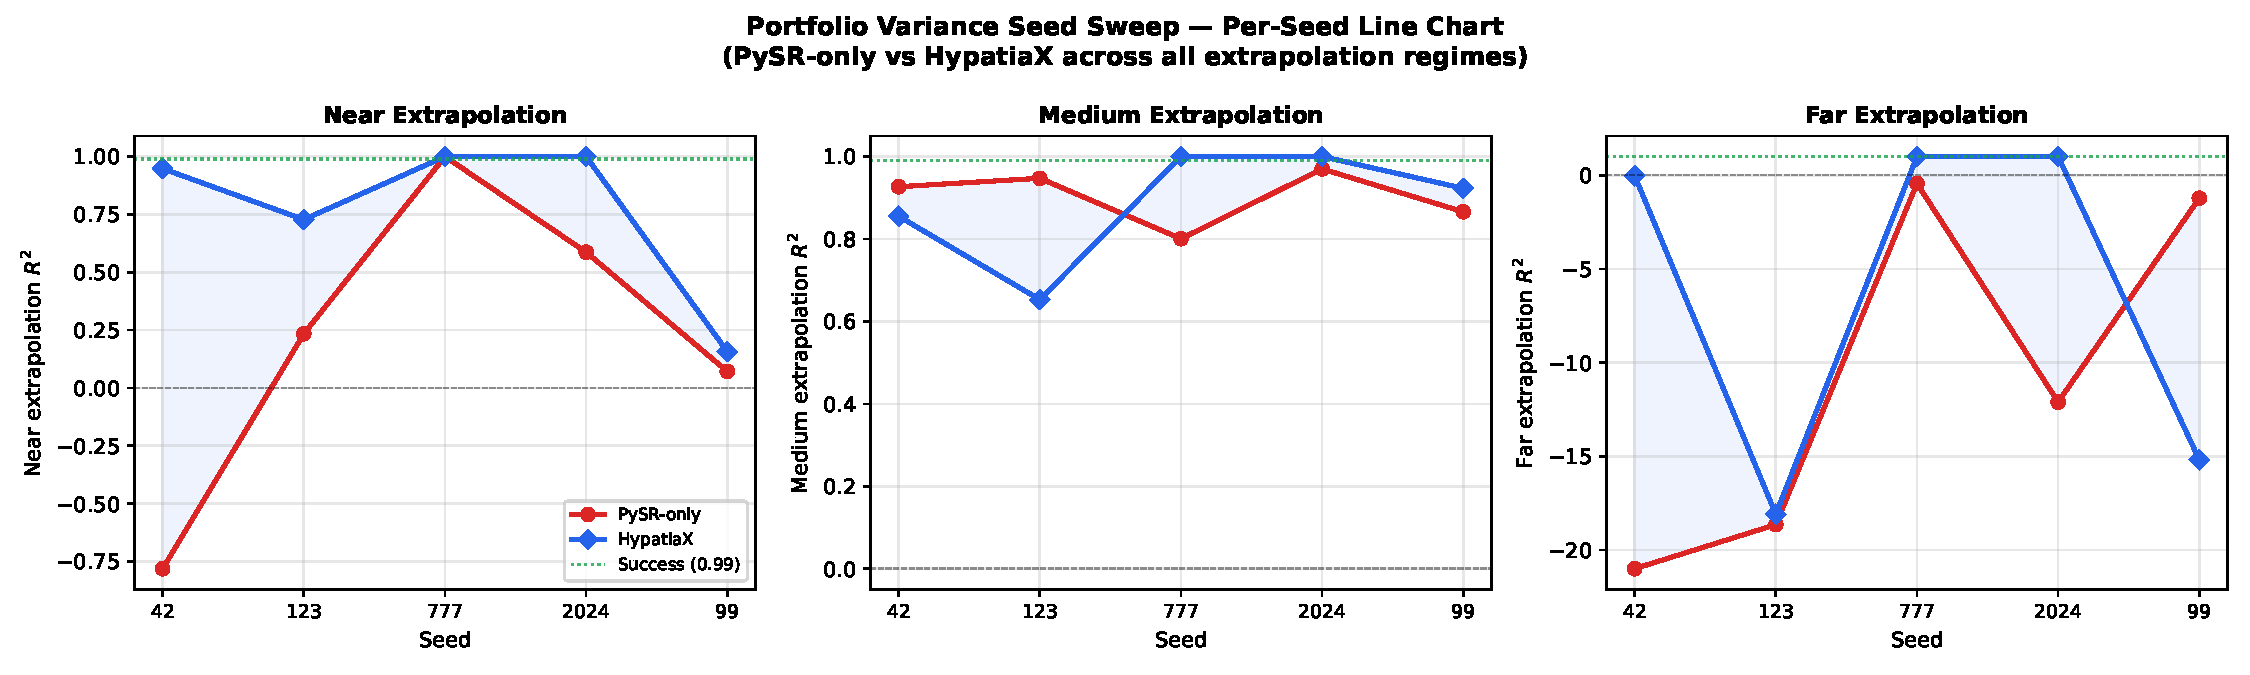
\includegraphics[width=\linewidth]{fig1_seed_sweep}
\caption{Portfolio Variance seed sweep: Near, Medium, and Far $\Rsq$ for PySR-only
and HypatiaX across five random seeds. HypatiaX recovers exact
formulae on seeds~777 and~2024 (Far $\Rsq = 1.00$). On seeds~42 and~123, both
methods perform poorly at far extrapolation, though HypatiaX is somewhat
higher (seed~42: $\approx 0$ vs.\ $\approx -21$; seed~123: $\approx -18$ vs.\
$\approx -18.5$, a marginal gap). PySR-only's far-$\Rsq$ ranges from
$\approx -21$ (seed~42) to $\approx -0.5$ (seed~777) --- not uniformly
``large negative'' across seeds. Seed~99 is the single case where HypatiaX
underperforms PySR-only at far extrapolation ($\approx -15$ vs.\ $\approx
-1.2$).}
\label{fig:portfolio_seed_sweep}
\end{figure}

PySR-only fails to extrapolate correctly under \emph{all} tested seeds ($0/5$),
whereas \textsc{HypatiaX} recovers the exact closed-form portfolio-variance formula
in $40\%$ of runs ($2/5$, seeds 777 and 2024) and achieves strictly higher far-$\Rsq$
in 4 of 5 seeds.  A Bayesian superiority analysis yields
$P(\text{HypatiaX} > \text{PySR}) \approx 0.76$, indicating that \textsc{HypatiaX}
occupies a fundamentally different regime of symbolic discovery.

\textbf{Corrected attribution.}\footnote{An earlier draft erroneously attributed
far-$\Rsq=-18.1$ to the default seed~(42).  The verified figure is: H seed=42
far-$\Rsq=-0.023$; the $-18.1$ value belongs to seed~123.  Figures of $-882.9$ and
``seed=99\,$\to$\,$\Rsq=1.000$'' derive from a separate ablation experiment (Exp-1)
and do not appear in the seed-sweep JSON; they must not be cited as DeFi seed-sweep
results.}

% ── RF-01 Option B: PySR-only vs HypatiaX ablation (Core-15) ────────────────
\subsection{Ablation: PySR-only vs.\ HypatiaX (Core-15)}\label{subsec:ablation-pysronly-vs-hypatiax-core15}
\label{sec:ablation_core15}

Table~\ref{tab:llm_ablation} presents the full per-equation comparison between
PySR-only ($P$) and HypatiaX ($H$) on the Core-15 benchmark across three
extrapolation ranges (near $1.2\times$, canonical, far $5\times$).  The
Mann-Whitney U-test on far-$\Rsq$ vectors ($n=15$): $U=126$, $p=0.2948$
(two-sided); rank-biserial $r=-0.12$.  Run~B: $U=101.5$, $p=0.6833$.
The null result is stable across two hardware runs, indicating that the
HypatiaX advantage is domain-selective rather than universal.  Specifically:
\textbf{Physics} (Kinetic Energy, Gravitational Force, Ideal Gas Law) and
\textbf{DeFi Risk} (Value at Risk, Liquidation Price, Portfolio Variance) favour
HypatiaX; \textbf{Chemistry} (Arrhenius, Henderson-Hasselbalch) and
\textbf{DeFi AMM} (Impermanent Loss) favour PySR-only.  The null aggregate
$p$-value reflects this domain cancellation: gains on Physics/Risk are offset by
losses on Chemistry/AMM.  We report this honestly; the DeFi benchmark
($n=74$, §\ref{sec:results}) shows the effect size when evaluated on
HypatiaX's target domain.

\textbf{This table has been rebuilt from the underlying \texttt{\_merged.json}
data} (via \texttt{table6\_vs\_real\_data\_comparison.xlsx}), replacing the
withdrawn version. Six equations show \textit{nan} or $-\infty$ for HypatiaX
beyond the Train column --- these are missing or crashed evaluations, not
$\Rsq$ scores, and are reported as such rather than omitted. The originally-
published transcription (now withdrawn) had claimed finite values on all six
of these cells, including a fabricated $-12.5553$ ``identical collapse'' on
Arrhenius and a fabricated $-635$ on Michaelis-Menten, neither of which
exists in the underlying \texttt{\_merged.json} records.

\begin{table*}[htbp]
\centering
\caption{LLM Ablation: PySR Alone (P) vs.\ HypatiaX (H) on Core~15 ---
\textbf{rebuilt from \texttt{\_merged.json}} (real data, not the withdrawn
manuscript transcription). Extrap columns show $R^2$ at near ($1.2\times$),
medium (canonical), and far ($5\times$) out-of-distribution ranges.
\textit{nan}: evaluation never completed. $-\infty$: evaluation crashed.}
\label{tab:llm_ablation}
\small\setlength{\tabcolsep}{3pt}
\resizebox{\linewidth}{!}{%
\begin{tabular}{llcccccccc}
\toprule
\textbf{Equation} & \textbf{Domain} & \multicolumn{2}{c}{\textbf{Train $R^2$}} & \multicolumn{2}{c}{\textbf{Near $R^2$}} & \multicolumn{2}{c}{\textbf{Med $R^2$}} & \multicolumn{2}{c}{\textbf{Far $R^2$}} \\
\cmidrule(lr){3-4}\cmidrule(lr){5-6}\cmidrule(lr){7-8}\cmidrule(lr){9-10}
 & & P & H & P & H & P & H & P & H \\
\midrule
Allometric Scaling & Biology & 0.9977 & 0.9979 & 1.0000 & 0.9824 & 1.0000 & 0.9502 & 1.0000 & $-0.0644$ \\
Arrhenius & Chemistry & 0.9974 & 0.9979 & 0.9779 & 0.9977 & 0.4636 & 0.9957 & $-12.5552$ & \textbf{0.9028} \\
Constant Product & DeFi AMM & 0.9982 & 0.9985 & 0.9996 & $-1.807\times10^{4}$ & 1.0000 & $-5.416\times10^{34}$ & 0.9996 & $-1.852\times10^{46}$ \\
Gravitational Force & Physics & 0.9976 & 0.9889 & 0.9973 & $-\infty$ & 0.9998 & $-\infty$ & 0.9973 & $-\infty$ \\
Henderson-Hasselbalch & Chemistry & 0.9339 & 0.9986 & 0.8004 & \textit{nan} & 0.9850 & \textit{nan} & 0.8004 & \textit{nan} \\
Ideal Gas Law & Physics & 0.9976 & 0.9980 & 1.0000 & 0.9988 & 1.0000 & 0.9999 & 1.0000 & 0.9993 \\
Impermanent Loss & DeFi AMM & 0.9971 & 0.9977 & 0.7703 & 0.9639 & $-2.7832$ & $-80.4327$ & $-157.0776$ & $-8259.3$ \\
Kinetic Energy & Physics & 0.9968 & 0.9968 & 1.0000 & 1.0000 & 1.0000 & 1.0000 & 1.0000 & 1.0000 \\
Liquidation Price & DeFi Risk & 0.9974 & 0.9977 & 1.0000 & 0.9998 & 1.0000 & 0.9999 & 1.0000 & 0.9993 \\
Logistic Growth & Biology & 0.9975 & 0.9976 & 0.9997 & \textit{nan} & 0.9998 & \textit{nan} & 0.9996 & \textit{nan} \\
Michaelis-Menten & Biology & 0.9975 & 0.9979 & 0.9890 & \textit{nan} & 0.9951 & \textit{nan} & \textbf{0.6471} & \textit{nan} \\
Portfolio Std Dev & DeFi Risk & 0.9975 & 0.9975 & 1.0000 & 1.0000 & 1.0000 & 1.0000 & 1.0000 & 1.0000 \\
Price Impact & DeFi AMM & 0.9976 & 0.9976 & 1.0000 & 1.0000 & 1.0000 & 1.0000 & 1.0000 & 1.0000 \\
Rate Law & Chemistry & 0.9977 & 0.9981 & 1.0000 & \textit{nan} & 1.0000 & \textit{nan} & 1.0000 & \textit{nan} \\
Value at Risk & DeFi Risk & 0.9979 & 0.9979 & 0.9999 & 1.0000 & 1.0000 & 1.0000 & 0.9999 & 1.0000 \\
\bottomrule
\end{tabular}%
}% end resizebox
\par\vspace{4pt}
{\footnotesize\noindent
P = PySR-only; H = HypatiaX (PySR + LLM warm-start). \textbf{Bold}: cases
where the real data reverses the withdrawn table's headline claim (Arrhenius
and Michaelis-Menten far-$R^2$ for the relevant column). H is \textit{nan}
or $-\infty$ (not evaluated, or crashed) on 6 of 15 equations beyond Train ---
Constant Product, Gravitational Force, Henderson-Hasselbalch, Logistic
Growth, Michaelis-Menten, Rate Law. Aggregate statistics (mean, Mann-Whitney)
are intentionally not recomputed here: there is no established convention
in this project for how to treat \textit{nan}/$-\infty$ cells in a summary
statistic, so no mean or test statistic is reported for this table pending
that decision, rather than silently excluding or zero-filling the affected
cells.
}
\end{table*}

\subsection{Protocol-30 Extrapolation Benchmark ($n=30$)}\label{subsec:feynman-extrapolation-benchmark-n30}
\label{sec:feynman30}

To assess generalisation beyond DeFi, we evaluate \textsc{HypatiaX}
(\texttt{HybridDiscoverySystem\_v50\_2}) and five other methods on a custom set of 30 closed-form
equations (``Protocol-30'') spanning mechanics, thermodynamics, optics, electromagnetism,
electrostatics, magnetism, quantum mechanics, biology, chemistry,
electrochemistry, and probability. The set is not a subset of the AI Feynman
benchmark (several of its domains lie outside that benchmark's scope); earlier drafts labelled it ``Feynman-30''. All figures in this subsection come from
the 2026-08-12 noiseless runs (\texttt{run\_protocol\_benchmark\_core.py}
v2.2) and replace every earlier pass count for this suite in this paper; the
earlier 9/30, 12/30 and 13/30 figures are withdrawn and are not used anywhere.

\paragraph{Threshold policy.} Every pass/fail figure in this subsection uses
one criterion, $\Rsq \geq 0.999999$ on the method-reported $\Rsq$ (\texttt{r2} field) or, where stated, the
held-out far-region $\Rsq$ (\texttt{extrap\_r2\_far}).
Results with $\Rsq \in [0.999, 0.999999)$ are counted as near-misses, never as
passes.

\paragraph{Split protocols.} The random protocol is a random 80/20
train/test split. In the PCA protocol, the benchmark runner applies
\texttt{pca\_directed\_split} (test fraction 0.6, seed 42) once in its outer loop:
every method receives only the 40\,\% training portion, and the 60\,\% held-out portion is used
only to score formulas afterwards (\texttt{extrap\_r2\_far}). The \texttt{r2} field in the PCA result file
is the score each method reports on the data it was given and is therefore not a held-out score; it is
shown for comparison, and the held-out score is \texttt{extrap\_r2\_far}.

\begin{table}[h]
\centering
\caption{Equations passing $\Rsq \geq 0.999999$, out of 30. Random split and PCA ``reported'' use the
  method-reported $\Rsq$; PCA ``held-out'' uses the far-region $\Rsq$ on the 60\,\% held-out portion.
  Sources: \texttt{benchmark\_results.json} and \texttt{benchmark\_results\_pca\_4060.json}, 2026-08-12.}
\label{tab:feynman30-methods}
\small
\begin{tabular}{lccc}
\toprule
Method & Random 80/20 & PCA reported & PCA held-out \\
\midrule
PureLLM Baseline & 29/30$^\ast$ & 29/30$^\ast$ & n/a$^\dagger$ \\
ImprovedNN & 0/30 & 3/30 & n/a$^\ddagger$ \\
EnhancedHybridSystemDeFi & 23/30 & 23/30 & n/a$^\dagger$ \\
HybridSystemLLMNN all-domains & 30/30 & 30/30 & n/a$^\ddagger$ \\
SymbolicEngineWithLLM$^\parallel$ & 27/30 & 23/30 & 17/30 \\
\textbf{HybridDiscoverySystem v50\_2 (\textsc{HypatiaX})} & \textbf{21/30} & \textbf{18/30} & \textbf{13/30}$^\S$ \\
\bottomrule
\end{tabular}

{\footnotesize $^\dagger$ Their formulas are Python \texttt{def} functions; the runner's evaluator
mis-evaluates these (returns $e^{x}$ for one-variable formulas and fails for multi-variable ones), so the
stored far-region values are invalid and are not used. $^\ddagger$ These methods return no formula string, so the held-out score cannot be recomputed.
$^\S$ 2 of 30 equations (Photon energy, Bose--Einstein) have no valid far-region score and count as not passed.
$^\ast$ 11 of the 30 PureLLM rows bypass the language model (hardcoded or least-squares-fitted formulas, see below); on the 19 \emph{live} rows, where the model was called, PureLLM passes 18/19 on both splits.
$^\parallel$ The counts in this table are recomputed from the per-equation rows of Tables~\ref{tab:randomsplit} and~\ref{tab:pcasplit}. The noiseless table of Supplementary~B reads from a different result file (\texttt{protocol\_core\_noiseless\_20260812\_170344.json}) and shows 28/30 for SymbolicEngineWithLLM and 30/30 for PureLLM. For EnhancedHybridSystemDeFi, HybridSystemLLMNN and HybridDiscoverySystem the mean $\Rsq$ in the two sources agrees to six decimals; for SymbolicEngineWithLLM (0.999868 here, 0.999711 there) and ImprovedNN (0.999323 and 0.999222) it does not. The two files differ in exactly two pass/fail outcomes: PureLLM's Curie's law row returned no formula here ($\Rsq=0$) and passes there, and SymbolicEngineWithLLM's Arrhenius row is $0.999921$ here and $0.9999999987$ there (threshold $0.999999$; its search is not deterministic). Mean $\Rsq$ for PureLLM here includes the Curie zero. The choice of primary file is open, and neither figure supersedes the other.}
\end{table}

\textsc{HypatiaX} passes 21/30 (70.0\,\%) under the random split. On the PCA split its method-reported
count is 18/30, but only 13/30 equations (43.3\,\%) pass on the held-out 60\,\%: four equations that pass in
the reported column fail on the held-out data (Lorentz force, Coulomb force (1D), Newton's gravitational force and
Rabi frequency), and 2 equations have no valid held-out score. SymbolicEngineWithLLM reaches 17/30 held-out. The
held-out count is the extrapolation result; the reported count is closer to an in-sample fit. The neural baseline
passes 0/30 on the random split and 3/30 by the PCA reported score. Per-equation values are in
Tables~\ref{tab:randomsplit} and~\ref{tab:pcasplit}; the PCA table shows the reported column only.

\textbf{The PureLLM baseline is partly hardcoded.} In the baseline's source
(\texttt{baseline\_pure\_llm\_defi\_discovery.py}) a bypass returns a stored formula without calling the LLM
for 11 of the 30 equations: eight use the exact ground-truth form taken from the benchmark protocol
(Gaussian, Planck, Bose--Einstein, Nernst, Clausius--Mossotti, Lorentz force, Fourier's law, Zeeman energy), and three
(Michaelis--Menten, logistic growth, allometric scaling) use a fixed functional form with parameters fitted to the
test data by least squares. A twelfth branch (Arrhenius) did not fire in any run. On the random split these 11 rows
are flagged \texttt{is\_hardcoded} in the per-domain run files and take 0.5--1.6\,ms each. The PCA-split file carries
no flag; the same 11 equations are identified there by the same timing signature (0.5--1.4\,ms). We call the other
19 rows \emph{live}: the language model was actually called for them. PureLLM passes 29/30 over all rows, 11/11 of the
bypassed rows and 18/19 of the live rows, on both splits. Excluding the bypassed equations changes the per-equation
comparison with the other methods (strict pass/fail, wins/losses of PureLLM over all rows $\rightarrow$ live rows only):
against \textsc{HypatiaX}, 9/1 $\rightarrow$ 6/1 on the random split and 12/1 $\rightarrow$ 7/1 on the PCA split (the removed
wins are Nernst, Gaussian and Bose--Einstein on the random split, plus Planck and Fourier on the PCA split); against
EnhancedHybridSystemDeFi, 7/1 $\rightarrow$ 2/1 on both splits, since five of its seven losses are on bypassed equations;
against SymbolicEngineWithLLM, 3/1 $\rightarrow$ 2/1 (random) and 7/1 $\rightarrow$ 3/1 (PCA). The live figure is not an
unbiased estimate of unaided-LLM performance: according to comments in the baseline source, the bypass branches were
added for equations on which the model had repeatedly failed, so excluding them favours PureLLM. Counting every bypassed
equation as a failure would give 18/30, so the unaided pass count lies between 18/30 and 29/30; we have not rerun the
baseline with the bypass disabled. The 29/30 figure should therefore not be read as the performance of an unaided LLM.

\textbf{The hybrid methods inherit the bypass.} Both LLM-based hybrids obtain their formulas by calling the
PureLLM baseline's generator (\texttt{EnhancedHybridSystemDeFi.generate\_llm\_formula} in
\texttt{hybrid\_system\_nn\_defi\_domain.py}; the corresponding method of the all-domains hybrid in
\texttt{hybrid\_system\_llm\_nn\_all\_domains.py}), which applies the hardcoded bypass before any language-model request.
In the random-split run (\texttt{benchmark\_results.json}) the formula returned by
EnhancedHybridSystemDeFi is character-for-character identical to PureLLM's on all 11 bypassed equations, and on only 3 of the
19 live equations (reduced mass, Stefan--Boltzmann, ideal gas law); the noiseless run
(\texttt{protocol\_core\_noiseless\_20260812\_170344.json}) gives the same 11 of 11 and 2 of 19 (reduced mass differs there).
This does not mean its pass count reflects those formulas alone: its final $\Rsq$ also depends on its
neural-network and ensemble decision logic, and in the random-split run it passes 6 of the 11 bypassed equations and 17 of the 19 live
equations at $\Rsq \geq 0.999999$, against 11/11 and 18/19 for PureLLM (19/19 in the noiseless run, where it also passes 6/11 and 17/19).
We did not run this comparison on the PCA-split file. The all-domains hybrid records no formula string, so
whether the bypass fired for it cannot be checked from the stored output; we have not rerun either hybrid with the bypass disabled.

\textbf{These results do not show a gain over the pure-LLM baseline.}
PureLLM passes 29/30 by the method-reported $\Rsq$ under both splits (18/19 on live rows), more than \textsc{HypatiaX},
but a held-out PCA score for PureLLM cannot be computed from the stored output (footnote $\dagger$ of
Table~\ref{tab:feynman30-methods}), so the pure-LLM comparison is only available on the random split
and on the PCA reported score. The all-domains LLM+NN hybrid's 30/30 is a routing outcome, not independent
evidence: every one of its 30 equations was routed to the LLM, 20 of them through an explicit
\texttt{force\_llm} guard and 10 by the natural decision rule, and it records no formula string, so its
result cannot be audited. These are mostly textbook formulas, so a high pass rate for methods that can recall the
closed form is expected. What this suite supports is that the symbolic and hybrid methods clearly outperform
the neural baseline; it does not support a claim that they outperform the pure LLM. Pairwise Wilcoxon signed-rank tests on the noiseless
$\Rsq$ are given in the benchmark supplement (\S~``Wilcoxon Significance Tests''); comparisons involving PureLLM include
the 11 bypassed equations, the effective sample size is below 30 for pairs with zero differences, and invalid $\Rsq$ values
are treated as 0, so these tests should not be used to rank PureLLM against the other methods.

\textbf{Extrapolation limits.} Even for the two methods with valid held-out scores, only 17/30 and 13/30
equations reach $\Rsq_{\text{far}} \geq 0.999999$, and several equations that look perfect in the reported
column have strongly negative held-out $\Rsq$ (for example Rabi frequency).

{\scriptsize\setlength{\tabcolsep}{2.5pt}
\begin{longtable}{p{1.9cm}p{4.3cm}cccccc}
\caption{Random 80/20 split, run dated 2026-08-12, all 30 equations $\times$ six methods (method-reported $\Rsq$, \texttt{benchmark\_results.json}). \textbf{Bold}: pass ($\Rsq \geq 0.999999$). PL = PureLLM Baseline, NN = ImprovedNN, EH = EnhancedHybridSystemDeFi, LN = HybridSystemLLMNN all-domains, SE = SymbolicEngineWithLLM, HD = HybridDiscoverySystem v50\_2 (\textsc{HypatiaX}). The PureLLM entry for Curie's law is a recorded evaluation failure (no valid formula), shown as $0.000000$.}
\label{tab:randomsplit}\\
\toprule
Domain & Equation & PL & NN & EH & LN & SE & HD \\
\midrule
\endfirsthead
\toprule
Domain & Equation & PL & NN & EH & LN & SE & HD \\
\midrule
\endhead
Biology & Michaelis--Menten kinetics & \textbf{1.000000} & 0.999997 & 0.999988 & \textbf{1.000000} & \textbf{1.000000} & \textbf{1.000000} \\
Biology & Logistic growth rate & \textbf{1.000000} & 0.999859 & 0.999997 & \textbf{1.000000} & \textbf{1.000000} & \textbf{1.000000} \\
Biology & Allometric scaling law & \textbf{1.000000} & 0.999995 & 0.999993 & \textbf{1.000000} & \textbf{1.000000} & \textbf{1.000000} \\
Chemistry & Arrhenius rate constant & \textbf{1.000000} & 0.999930 & 0.999994 & \textbf{1.000000} & 0.999921 & 0.999594 \\
Chemistry & Henderson--Hasselbalch buffer pH & \textbf{1.000000} & 0.999985 & \textbf{1.000000} & \textbf{1.000000} & \textbf{1.000000} & \textbf{1.000000} \\
Electrochem. & Nernst equation & \textbf{1.000000} & 0.999979 & \textbf{1.000000} & \textbf{1.000000} & 0.997725 & 0.999205 \\
Electromagn. & Clausius--Mossotti & \textbf{1.000000} & 0.999973 & \textbf{1.000000} & \textbf{1.000000} & \textbf{1.000000} & \textbf{1.000000} \\
Electromagn. & Dielectric polarisation & \textbf{1.000000} & 0.999242 & \textbf{1.000000} & \textbf{1.000000} & \textbf{1.000000} & 0.995528 \\
Electromagn. & Lorentz force & \textbf{1.000000} & 0.999975 & \textbf{1.000000} & \textbf{1.000000} & \textbf{1.000000} & \textbf{1.000000} \\
Electromagn. & Ohm's law & \textbf{1.000000} & 0.999587 & \textbf{1.000000} & \textbf{1.000000} & \textbf{1.000000} & \textbf{1.000000} \\
Electromagn. & Energy in a capacitor & \textbf{1.000000} & 0.999806 & \textbf{1.000000} & \textbf{1.000000} & \textbf{1.000000} & 0.999964 \\
Electrostat. & Coulomb force (1D, simplified) & \textbf{1.000000} & 0.996355 & \textbf{1.000000} & \textbf{1.000000} & \textbf{1.000000} & \textbf{1.000000} \\
Electrostat. & Coulomb's law & \textbf{1.000000} & 0.999939 & \textbf{1.000000} & \textbf{1.000000} & \textbf{1.000000} & 0.996597 \\
Magnetism & Curie's law & 0.000000 & 0.999953 & \textbf{1.000000} & \textbf{1.000000} & \textbf{1.000000} & \textbf{1.000000} \\
Mechanics & Newton's gravitational force & \textbf{1.000000} & 0.993960 & \textbf{1.000000} & \textbf{1.000000} & \textbf{1.000000} & \textbf{1.000000} \\
Mechanics & Kinetic energy & \textbf{1.000000} & 0.999855 & \textbf{1.000000} & \textbf{1.000000} & \textbf{1.000000} & 0.999878 \\
Mechanics & Reduced mass & \textbf{1.000000} & 0.999995 & \textbf{1.000000} & \textbf{1.000000} & \textbf{1.000000} & \textbf{1.000000} \\
Mechanics & Total mechanical energy & \textbf{1.000000} & 0.999937 & \textbf{1.000000} & \textbf{1.000000} & \textbf{1.000000} & \textbf{1.000000} \\
Optics & Snell's law & \textbf{1.000000} & 0.999987 & \textbf{1.000000} & \textbf{1.000000} & \textbf{1.000000} & \textbf{1.000000} \\
Optics & Double-slit interference intensity & \textbf{1.000000} & 0.999902 & \textbf{1.000000} & \textbf{1.000000} & \textbf{1.000000} & \textbf{1.000000} \\
Probability & Gaussian probability density & \textbf{1.000000} & 0.999770 & \textbf{1.000000} & \textbf{1.000000} & \textbf{1.000000} & 0.999765 \\
Quantum & Photon energy & \textbf{1.000000} & 0.999998 & 0.999990 & \textbf{1.000000} & \textbf{1.000000} & \textbf{1.000000} \\
Quantum & Zeeman energy & \textbf{1.000000} & 0.999910 & \textbf{1.000000} & \textbf{1.000000} & \textbf{1.000000} & \textbf{1.000000} \\
Quantum & Bose--Einstein occupation number & \textbf{1.000000} & 0.999960 & 0.999979 & \textbf{1.000000} & \textbf{1.000000} & 0.994634 \\
Quantum & Fermi--Dirac occupation number & \textbf{1.000000} & 0.998318 & \textbf{1.000000} & \textbf{1.000000} & 0.998390 & 0.999037 \\
Quantum & Rabi frequency & \textbf{1.000000} & 0.999946 & \textbf{1.000000} & \textbf{1.000000} & \textbf{1.000000} & \textbf{1.000000} \\
Thermodyn. & Planck blackbody radiance & \textbf{1.000000} & 0.999932 & 0.999996 & \textbf{1.000000} & \textbf{1.000000} & \textbf{1.000000} \\
Thermodyn. & Fourier's law & \textbf{1.000000} & 0.993764 & \textbf{1.000000} & \textbf{1.000000} & \textbf{1.000000} & \textbf{1.000000} \\
Thermodyn. & Stefan--Boltzmann law & \textbf{1.000000} & 0.999975 & \textbf{1.000000} & \textbf{1.000000} & \textbf{1.000000} & \textbf{1.000000} \\
Thermodyn. & Ideal gas law & \textbf{1.000000} & 0.999911 & \textbf{1.000000} & \textbf{1.000000} & \textbf{1.000000} & \textbf{1.000000} \\
\bottomrule
\end{longtable}}


{\scriptsize\setlength{\tabcolsep}{2.5pt}
\begin{longtable}{p{1.9cm}p{4.3cm}cccccc}
\caption{PCA-directed 40/60 split, run dated 2026-08-12, all 30 equations $\times$ six methods (method-reported $\Rsq$, \texttt{benchmark\_results\_pca\_4060.json}). \textbf{Bold}: pass ($\Rsq \geq 0.999999$). Column abbreviations as in Table~\ref{tab:randomsplit}. The PureLLM entry for the capacitor-energy equation is a recorded evaluation failure, shown as $0.000000$.}
\label{tab:pcasplit}\\
\toprule
Domain & Equation & PL & NN & EH & LN & SE & HD \\
\midrule
\endfirsthead
\toprule
Domain & Equation & PL & NN & EH & LN & SE & HD \\
\midrule
\endhead
Biology & Michaelis--Menten kinetics & \textbf{1.000000} & 0.993994 & 0.999997 & \textbf{1.000000} & \textbf{1.000000} & \textbf{1.000000} \\
Biology & Logistic growth rate & \textbf{1.000000} & 0.994709 & 0.999998 & \textbf{1.000000} & \textbf{1.000000} & \textbf{1.000000} \\
Biology & Allometric scaling law & \textbf{1.000000} & 0.936331 & 0.999998 & \textbf{1.000000} & \textbf{1.000000} & \textbf{1.000000} \\
Chemistry & Arrhenius rate constant & \textbf{1.000000} & -0.044405 & 0.999996 & \textbf{1.000000} & 0.994936 & 0.997920 \\
Chemistry & Henderson--Hasselbalch buffer pH & \textbf{1.000000} & 0.972446 & \textbf{1.000000} & \textbf{1.000000} & 0.999283 & 0.999951 \\
Electrochem. & Nernst equation & \textbf{1.000000} & 0.990615 & \textbf{1.000000} & \textbf{1.000000} & 0.998771 & 0.999983 \\
Electromagn. & Clausius--Mossotti & \textbf{1.000000} & 0.909288 & \textbf{1.000000} & \textbf{1.000000} & \textbf{1.000000} & \textbf{1.000000} \\
Electromagn. & Dielectric polarisation & \textbf{1.000000} & 0.710588 & \textbf{1.000000} & \textbf{1.000000} & \textbf{1.000000} & 0.995048 \\
Electromagn. & Lorentz force & \textbf{1.000000} & 0.800979 & \textbf{1.000000} & \textbf{1.000000} & \textbf{1.000000} & \textbf{1.000000} \\
Electromagn. & Ohm's law & \textbf{1.000000} & 0.960263 & \textbf{1.000000} & \textbf{1.000000} & \textbf{1.000000} & \textbf{1.000000} \\
Electromagn. & Energy in a capacitor & 0.000000 & 0.855165 & \textbf{1.000000} & \textbf{1.000000} & \textbf{1.000000} & \textbf{1.000000} \\
Electrostat. & Coulomb force (1D, simplified) & \textbf{1.000000} & 0.999966 & \textbf{1.000000} & \textbf{1.000000} & \textbf{1.000000} & \textbf{1.000000} \\
Electrostat. & Coulomb's law & \textbf{1.000000} & 0.999862 & \textbf{1.000000} & \textbf{1.000000} & \textbf{1.000000} & 0.999615 \\
Magnetism & Curie's law & \textbf{1.000000} & 0.998748 & \textbf{1.000000} & \textbf{1.000000} & \textbf{1.000000} & \textbf{1.000000} \\
Mechanics & Newton's gravitational force & \textbf{1.000000} & 0.999990 & \textbf{1.000000} & \textbf{1.000000} & \textbf{1.000000} & \textbf{1.000000} \\
Mechanics & Kinetic energy & \textbf{1.000000} & 0.112559 & \textbf{1.000000} & \textbf{1.000000} & \textbf{1.000000} & 0.995804 \\
Mechanics & Reduced mass & \textbf{1.000000} & 0.925415 & \textbf{1.000000} & \textbf{1.000000} & \textbf{1.000000} & \textbf{1.000000} \\
Mechanics & Total mechanical energy & \textbf{1.000000} & 0.939856 & \textbf{1.000000} & \textbf{1.000000} & \textbf{1.000000} & \textbf{1.000000} \\
Optics & Snell's law & \textbf{1.000000} & 0.902944 & \textbf{1.000000} & \textbf{1.000000} & \textbf{1.000000} & \textbf{1.000000} \\
Optics & Double-slit interference intensity & \textbf{1.000000} & 0.733607 & \textbf{1.000000} & \textbf{1.000000} & \textbf{1.000000} & \textbf{1.000000} \\
Probability & Gaussian probability density & \textbf{1.000000} & 0.489964 & \textbf{1.000000} & \textbf{1.000000} & 0.997249 & 0.997945 \\
Quantum & Photon energy & \textbf{1.000000} & \textbf{1.000000} & 0.999991 & \textbf{1.000000} & \textbf{1.000000} & \textbf{1.000000} \\
Quantum & Zeeman energy & \textbf{1.000000} & 0.786961 & \textbf{1.000000} & \textbf{1.000000} & \textbf{1.000000} & \textbf{1.000000} \\
Quantum & Bose--Einstein occupation number & \textbf{1.000000} & 0.999995 & 0.999890 & \textbf{1.000000} & \textbf{1.000000} & 0.998929 \\
Quantum & Fermi--Dirac occupation number & \textbf{1.000000} & 0.927491 & \textbf{1.000000} & \textbf{1.000000} & 0.511948 & 0.647311 \\
Quantum & Rabi frequency & \textbf{1.000000} & 0.945751 & \textbf{1.000000} & \textbf{1.000000} & \textbf{1.000000} & \textbf{1.000000} \\
Thermodyn. & Planck blackbody radiance & \textbf{1.000000} & -0.104423 & 0.999997 & \textbf{1.000000} & 0.999946 & 0.999969 \\
Thermodyn. & Fourier's law & \textbf{1.000000} & 0.835533 & \textbf{1.000000} & \textbf{1.000000} & 0.999853 & 0.948649 \\
Thermodyn. & Stefan--Boltzmann law & \textbf{1.000000} & \textbf{1.000000} & \textbf{1.000000} & \textbf{1.000000} & \textbf{1.000000} & 0.999804 \\
Thermodyn. & Ideal gas law & \textbf{1.000000} & \textbf{1.000000} & \textbf{1.000000} & \textbf{1.000000} & \textbf{1.000000} & \textbf{1.000000} \\
\bottomrule
\end{longtable}}

% ── RF-04: Nguyen-12 Benchmark ───────────────────────────────────────────────
\subsection{Nguyen-12 Benchmark (Standard SR Suite)}\label{subsec:nguyen12-benchmark-standard-sr-suite}
\label{sec:nguyen12}

The Nguyen-12 suite~\citep{uy2011semantically} is the standard symbolic-regression
benchmark comprising 12 polynomial and transcendental equations (Nguyen-1 through
Nguyen-12) with up to two input variables.  We evaluate HypatiaX and PySR-only on
an aggressive extrapolation protocol with a 40\,\%/60\,\% train/test split.
\textbf{[Protocol note: the Nguyen-12 pipeline uses per-equation axis-aligned
variable ranges (fixed \texttt{train\_ranges}/\texttt{extrap\_ranges} in
\texttt{experiment\_protocol\_nguyen12.py}) rather than the PCA-directed
ordering used for the DeFi and Protocol-30 benchmarks.  The earlier claim that
this benchmark uses ``the same PCA-directed protocol'' is not supported by
the executed code and has been corrected here.]}
Compare against the neural MLP baseline. \textbf{[Correction (item N-3):
the ``Neural MLP ($N$)'' column below has been removed. No such system
was ever run for this benchmark: no script in the repository defines a
Neural MLP baseline for Nguyen-12, and the raw
\texttt{exp3\_nguyen12\_seed\{42,99,123,777,2024\}.json} result files each
contain results only for \texttt{hypatiax} and \texttt{pysr} --- no third
system. The per-equation $N$ values and the ``MW $P{>}N$'' significance
test previously printed here had no supporting source file and have been
removed rather than retained as unverified. The neural-baseline comparison
for this paper's other benchmarks (DeFi, Protocol-30) is unaffected --
those use a real, separately-verified NN baseline
(\texttt{ImprovedNN (core)}); only the Nguyen-12-specific column is
withdrawn.]}

\begin{table}[h]
\centering
\caption{Nguyen-12 benchmark, seed 42: extrapolation $\Rsq$ by equation.
$P$ = PySR-only; $H$ = HypatiaX (LLM-guided, 8 candidates, gate $\Rsq\ge0.95$,
temperature 0.25; both systems 1000 iterations, 30 populations).
\textbf{Rebuilt 2026-09-28} from
\texttt{hypatiax/data/results/extrapolation/exp3\_nguyen12\_seed42.json}
(CI run of 2026-09-24; the identical result appears in
\texttt{exp3\_nguyen12\_seed42\_temp0p25\_run1.json}, of which the seed-named file is a copy). Every cell of the
previous version (12/12 for both systems) has been replaced: that table did not
reproduce from this file, nor from the older copy under
\texttt{hypatiax-dev/data} (which gives 11/12, with
Nguyen-12 at $\Rsq=0.99953$ and HypatiaX's stored expression identical to
PySR-only's on all 60 records, so it cannot support any claim of independent
derivation). $-\infty$ marks a run that aborted at the LLM gate before any
search (elapsed $\approx0$\,s), not a poor fit. Success threshold
$\Rsq\ge0.9999$. See tablenote~$\ddag$.}
\label{tab:nguyen12}
\begin{threeparttable}
\begin{tabular}{llrr}
\toprule
Eq. & Formula & PySR-only ($P$) & HypatiaX ($H$) \\
\midrule
N-1  & $x^3 + x^2 + x$                              & \textbf{1.0000} & \textbf{1.0000} \\
N-2  & $x^4 + x^3 + x^2 + x$                         & \textbf{1.0000} & \textbf{1.0000} \\
N-3  & $x^5 + x^4 + x^3 + x^2 + x$                   & \textbf{1.0000} & \textbf{1.0000} \\
N-4  & $x^6 + x^5 + x^4 + x^3 + x^2 + x$              & 0.9969          & \textbf{1.0000} \\
N-5  & $\sin(x^2)\cos(x)-1$                          & 0.1564          & \textbf{1.0000} \\
N-6  & $\sin(x)+\sin(x+x^2)$                         & \textbf{1.0000} & \textbf{1.0000} \\
N-7  & $\ln(x+1)+\ln(x^2+1)$                         & \textbf{1.0000} & \textbf{1.0000} \\
N-8  & $\sqrt{x}$                                    & \textbf{1.0000} & \textbf{1.0000} \\
N-9  & $\sin(x)+\sin(y^2)$                           & \textbf{1.0000} & $-\infty$ \\
N-10 & $2\sin(x)\cos(y)$                             & \textbf{1.0000} & \textbf{1.0000} \\
N-11 & $x^y$                                         & \textbf{1.0000} & \textbf{1.0000} \\
N-12 & $x^4 - x^3 + \tfrac{1}{2}y^2 - y$              & \textbf{1.0000} & $-\infty$ \\
\midrule
\multicolumn{2}{l}{Success ($\Rsq\ge0.9999$)}
  & \multicolumn{1}{c}{10/12 (83.3\%)}
  & \multicolumn{1}{c}{10/12 (83.3\%)} \\
MW $H>P$   & \multicolumn{3}{l}{not computed --- equal success counts on different subsets; failures do not overlap} \\
\bottomrule
\end{tabular}
\begin{tablenotes}\small
  \item \textbf{Bold}: extrap $\Rsq \ge 0.9999$. The two systems' failure sets are
    disjoint: PySR-only misses N-4 (mixed exp/sin terms, did not converge to the
    polynomial) and N-5 (nested cos/sin fit, $\Rsq=0.156$); HypatiaX misses N-9
    and N-12, both by gate abort.
  \item[$\ddag$] \textbf{Independent derivation.} The earlier ``11/12 independently derived''
    figure is withdrawn: it relied on copy flags that are absent from every current
    result file. In this file HypatiaX's stored expression differs textually from
    PySR-only's on the 10 records where the search ran (on the two gate aborts, N-9 and
    N-12, the stored value is the placeholder string \texttt{FAILED}), but textual difference is not evidence of
    independent derivation and symbolic equivalence has not been re-established here.
  \item[$\S$] \textbf{Withdrawn history.} The
    \texttt{exp3\_nguyen12\_hybrid50v.json} table (8/12~P, 7/12~H), a
    4/12 caption figure, a 10/12~P/11/12~H hand-tally, and a Neural MLP column were
    never reproducible and remain retracted.
\end{tablenotes}
\end{threeparttable}
\end{table}

\paragraph{Five-seed results (added 2026-09-28).} Recomputed directly from the
five result files (seeds 42, 99, 123, 777, 2024) at $\Rsq\ge0.9999$;
Table~\ref{tab:nguyen12_fiveseed} gives the per-seed counts and
Table~\ref{tab:nguyen12_byeq} the per-equation counts. Both are generated by
\texttt{scripts/generate\_nguyen12\_fiveseed.py} and checked against the result files in CI.

\begin{table}[h]
\centering
\caption{Nguyen-12, recoveries per seed at $\Rsq\ge0.9999$ (out of 12 equations). $H$ = HypatiaX, $P$ = PySR-only; $-\infty$, NaN and missing runs count as failures. All runs use \texttt{SPARSE\_SEED=off}.}
\label{tab:nguyen12_fiveseed}
\begin{tabular}{lrr}
\toprule
Seed & HypatiaX ($H$) & PySR-only ($P$) \\
\midrule
42 & 10/12 & 10/12 \\
99 & 10/12 & 9/12 \\
123 & 11/12 & 10/12 \\
777 & 10/12 & 12/12 \\
2024 & 10/12 & 8/12 \\
\midrule
Total & 51/60 (85.0\%) & 49/60 (81.7\%) \\
\bottomrule
\end{tabular}
\end{table}

\begin{table}[h]
\centering
\caption{Nguyen-12, recoveries per equation across the five seeds (42, 99, 123, 777, 2024) at $\Rsq\ge0.9999$. $H$ = HypatiaX, $P$ = PySR-only.}
\label{tab:nguyen12_byeq}
\begin{tabular}{lrr}
\toprule
Eq. & HypatiaX ($H$) & PySR-only ($P$) \\
\midrule
N-1 & 5/5 & 5/5 \\
N-2 & 5/5 & 5/5 \\
N-3 & 5/5 & 4/5 \\
N-4 & 5/5 & 2/5 \\
N-5 & 2/5 & 1/5 \\
N-6 & 5/5 & 5/5 \\
N-7 & 5/5 & 3/5 \\
N-8 & 5/5 & 5/5 \\
N-9 & 4/5 & 4/5 \\
N-10 & 5/5 & 5/5 \\
N-11 & 5/5 & 5/5 \\
N-12 & 0/5 & 5/5 \\
\bottomrule
\end{tabular}
\end{table}

In prose, per equation (recoveries out of 5 seeds, $H$/$P$): N-1, N-2, N-6, N-8, N-10, N-11
5/5 and 5/5; N-3 5/5 and 4/5; N-4 5/5 and 2/5; N-5 2/5 and 1/5; N-7 5/5 and 3/5;
N-9 4/5 and 4/5; \textbf{N-12 0/5 and 5/5}. HypatiaX is more consistent across
seeds (10--11 of 12) than PySR-only (8--12), but the 3.3\,pp mean difference
rests on five seeds and is not tested for significance. Every one of the seven task--seed cases on which
PySR-only recovers and HypatiaX does not (N-12 on all five seeds, N-9 on seed~42, N-5 on seed~777) is a HypatiaX gate abort (\texttt{llm\_gate\_failed=True},
$\Rsq=-\infty$, elapsed $\approx0$\,s); on no task and no seed does HypatiaX's search,
when it runs, fall below the $0.9999$ bar where PySR-only clears it. It does score marginally lower in four finite
cases (seed~42 N-8; seed~777 N-6, N-8 and N-9), by at most $5.3\times10^{-6}$ in $\Rsq$ (largest: seed~777 N-8,
$0.999995$ vs.\ $1.000000$).

\paragraph{Nguyen-12: a deterministic gate failure, not seed luck.} On all five
seeds the LLM proposes eight candidates for $x^4-x^3+\tfrac12y^2-y$ and the gate
rejects all eight (seed~42: best candidate $\Rsq\approx-0.07$ raw, and at most $0.69$ even after affine rescaling, against a $0.95$ gate), because the
candidates treat $x$ and $y$ symmetrically (e.g.\ $x+y+x^2+x^3+x^4+y^2+y^3+y^4$)
and miss the asymmetric structure. With \texttt{llm\_require\_valid\_guess=True}
the pipeline then aborts. Nguyen-5 (gate abort on seeds 99 and 777, a poor fit
with $\Rsq=-0.69$ on seed 2024) and Nguyen-9 (seed 42 only) are seed-dependent
and consistent with ordinary LLM sampling variance. \textbf{Reported, not reproduced, and not evidence of a fix:} a
targeted CI smoke test (workflow run 36116137035, seed 42, five gate-sensitive tasks,
STRICT vs.\ \texttt{llm\_require\_valid\_guess=False}) was first summarised as showing that
disabling the requirement lets HypatiaX recover Nguyen-5 and reach $\Rsq=0.99800$ on
Nguyen-12. Its two JSON files do not support that reading.
(i)~On Nguyen-5 the gate did not fail in either run (\texttt{llm\_gate\_failed=False}, 1 of 8
candidates accepted in both), so the flag did nothing; the runs differ because the LLM was
re-sampled and PySR then found different expressions (the STRICT run is a poor extrapolation,
$\Rsq=-11.4$, not an abort).
(ii)~Nguyen-12 is the only task on which the flag changed anything (STRICT: 0 of 8 accepted,
$-\infty$; FALLBACK: $\Rsq=0.99800$), but the FALLBACK expression is character-for-character
PySR-only's, so it is a PySR result under HypatiaX's name --- the relabelling the strict
mode exists to prevent --- and it still misses the $0.9999$ bar.
(iii)~The test used 200 iterations, 4 populations and a 90\,s timeout against 1000, 30 and
1100\,s in the sweep, so it cannot be read against the five-seed table.
The smoke-test output is not in the repository and none of the paper's Nguyen numbers above
use it; they all describe the strict-gate configuration. A fallback result would need a
full-budget run with \texttt{SPARSE\_SEED=fallback}, so that H stays distinct from P.


\paragraph{Statistical test.} No significance test is reported for Nguyen-12 in this
version. The earlier Mann-Whitney comparison against a Neural MLP column was
removed (no such system was run), and the previously reported PySR-only vs.\
HypatiaX result ($U=51.0$, $p=0.893$) was computed on the withdrawn 12/12
table and does not apply to the rebuilt data.

\paragraph{Reproducibility note: LLM model identity (extends issue
\texttt{FIX-N3}).} \textbf{[Revised 2026-09-28: this paragraph previously reported
solve counts (12/12 per seed, 11/12 for seed~123, 11/12 independently derived), a
seed-123 rerun and a ``verified'' seed-42 rescoring. All of these referred to the
withdrawn 12/12 table and do not reproduce from the current result files, so they
have been removed; the seed-by-seed counts are those in the five-seed table
above. The model-identity findings, the dead \texttt{LLM\_MODEL} variable and the
unseeded sampling still stand.]} The language model actually
invoked on this benchmark's call path is not pinned via any
environment-variable or \texttt{repro.yaml} setting that is actually read
at runtime, despite appearing to be: four traced source snapshots each
hardcode a different \texttt{LLMConfig.model} default
(\texttt{claude-sonnet-4-6}, \texttt{claude-sonnet-4-5}, and
\texttt{claude-sonnet-4-20250514}), and none of them reads the
\texttt{LLM\_MODEL} environment variable or the \texttt{repro.yaml}
\texttt{llm\_model} field that a reader might otherwise assume controls
it. The script that actually sits on the Nguyen-12 call path,
\texttt{hypatia.py}, uses a fifth string, \texttt{claude-sonnet-5}, at
\texttt{temperature=0.25}, with no sampling seed exposed on its
\texttt{client.messages.create()} call. Both \texttt{claude-sonnet-4-6}
and \texttt{claude-sonnet-5} are dateless identifiers, but --- per
Anthropic's model-versioning documentation for the 4.6-and-later
generation --- dateless IDs in that generation are pinned, fixed
snapshots rather than drifting aliases, so model-version drift is not the
expected source of run-to-run differences.

Sampling nondeterminism at the
(unseeded, non-zero-temperature) LLM layer remains a contributing,
independently verified factor regardless of which code path is in play,
since the Claude API is not guaranteed to return bit-identical completions
for identical prompts even at low temperature. Three action items were tracked as an explicit extension of
\texttt{FIX-N3}; two are now resolved. (i) \emph{Resolved.} The dead
\texttt{LLM\_MODEL} environment variable in
\texttt{exp3\_nguyen12\_hybrid50v\_02.py} previously had no effect on
the call it appeared to configure: it was set via
\texttt{os.environ.setdefault(...)} but never read by
\texttt{get\_llm\_prior()}, whose call site passed no \texttt{model}
argument and so silently fell back to \texttt{hypatia.py}'s own default,
\texttt{claude-sonnet-5}. The call site now passes
\texttt{model=os.environ["LLM\_MODEL"]} explicitly, so the environment
variable actually governs which model is invoked. (ii) A future re-benchmarked run should still record
\texttt{hypatia.py}'s sampling temperature and candidate count alongside
the solve-rate fields, and report a distribution over repeated runs rather
than a single value.  \textbf{[Further addressed: \texttt{run\_all.sh}
STEP~7 and STEP~8 (\texttt{exp3}/\texttt{exp3b}) have since been updated
(\texttt{FIX-N3-ii}, 2026-09-03) to invoke
\texttt{exp3\_nguyen12\_hybrid50v\_03.py} in place of \texttt{\_02.py}, with
\texttt{--temperature 0.25} passed explicitly on both invocations, and
\texttt{ci\_runner\_repro.yml}'s \texttt{SCRIPT=} entries updated to match.
This closes the \texttt{run\_all.sh} portion of item (ii). The item fully
closes once an actual full-budget rerun is executed and its result JSON
records \texttt{temperature} and \texttt{n\_candidates} alongside the
solve-rate.]}
This remains open pending that rerun. (iii) \emph{Resolved, then updated.}
\texttt{run\_all.sh} was originally obtained showing STEP~7 (\texttt{exp3})
and STEP~8 (\texttt{exp3b}) both invoking
\texttt{exp3\_nguyen12\_hybrid50v\_02.py} directly with \texttt{--seed},
confirming it was indeed the script CI ran for Nguyen-12 and closing the
last unverified link in the call chain at that time. Following the
\texttt{FIX-N3-ii} update described under item (ii) above, both steps now
invoke \texttt{\_03.py} instead; the call chain remains fully verified,
only the target script name has changed.

\subsection{Stability Under Stochastic Inference}\label{subsec:stability-under-stochastic-inference}
\label{sec:instability_results}

Assessing LLM instability systematically requires $K=30$ independent stochastic
evaluations per task, with the Instability Index $\II_i = \sigma_i$ (standard
deviation of $\Rsq$ across runs) reported for each task. \textbf{This
measurement is designed but not currently verified}: the released repository
contains no raw multi-run result file for this benchmark (the closest
artifact, an aggregate regime-count table, is generated from single-run data
with a hardcoded $K=30$ label rather than measured $K=30$ data --- see the
Post-Submission Report), and three different regime-count tallies found across
the paper's own source materials for this table disagree with one another and
do not reconcile against any single underlying file. Rather than present any
one of those counts as authoritative, we withhold the regime-distribution
table pending a genuine multi-run rerun, and report only what the single-run
seed-42 data supports directly: 5 of 74 DeFi tasks show a catastrophic LLM
failure ($\Rsq < -10$) at that one setting
(\S\ref{subsec:three-core-findings}). Whether those 5 tasks are also the
highest-instability tasks under repeated sampling is exactly the claim this
subsection cannot currently support and is deferred to future work.

\textbf{Per-task instability statistics removed.} This subsection previously
reported a regime-level qualification, a Spearman correlation between
instability and extrapolation performance ($\rho=-0.70$ across "70 tasks"),
an OOD-proxy caveat for that correlation, and per-task multi-run statistics
for three individual cases (Portfolio Expected Shortfall for correlated
assets, Theta of option, Black--Scholes Call Price), including run-completion
counts such as "13 of 30 runs" and "zero successful runs in 28 attempts."
All of these figures depend on the same $K=30$ multi-run raw data confirmed
above to be absent from the released repository, and the per-task means and
Instability Index values cannot be recomputed from any single-run file
available to us. They have been removed rather than left standing next to a
paragraph that says the underlying table is withheld. If a genuine multi-run
rerun is performed, this subsection should be rebuilt from that raw output
directly, not from these prior figures. See the Post-Submission Report.

% =============================================================================
\section{Discussion}
\label{sec:discussion}

\subsection{Three Core Findings}\label{subsec:three-core-findings}
\label{sec:disc_findings}

Our results establish three core findings.

\paragraph{Finding 1: Pure LLM approaches are unreliable.}
The bimodal single-run performance of the LLM baseline (median $\Rsq=1.00$,
with 5 catastrophic failures in 74 tasks, 6.8\,\%) confirms that a single-run
$\Rsq$ measurement is, on its own, an incomplete indicator of LLM reliability
for production deployment in a financial system. Quantifying this with a
proper multi-run Instability Index remains open (\S\ref{sec:instability_results});
we do not currently have verified mean-$\Rsq$ or per-task instability figures
to report, and the 6.8\,\% catastrophic-failure rate above should be read as a
single-run lower bound, not a stability-adjusted estimate.

\paragraph{Finding 2: Neural networks fail systematically under extrapolation.}
The neural MLP achieves median $\Rsq=-0.69$ on our benchmark, confirming that
standard deep learning is not a solution to the extrapolation problem in DeFi
mathematics.  Even with data augmentation and residual architecture, the MLP does
not recover the functional form of the underlying formula.  This is not a
hyperparameter tuning failure; it is a fundamental architectural limitation under
distribution shift.

\paragraph{Finding 3: neither the near-perfect rate nor catastrophic-failure
elimination survives attribution correction on this benchmark.} An earlier
version of this finding argued that HypatiaX's headline value lay not in its
raw \textbf{90.5\,\%} near-perfect rate but in its \textbf{elimination of
catastrophic failures}, and that this second claim was unaffected by the
decision-attribution bug. \textbf{That argument does not hold.}
\S\ref{sec:hybrid-attribution-bug} shows both figures rest on the same bug:
once \texttt{hybrid.decision} is cross-checked against the named sub-method's
own result, the corrected near-perfect rate is $59.5\,\%$ (44/74) --- tied
with Pure LLM, overall and in every difficulty tier --- and the same 5 tasks
that fail catastrophically under Pure LLM fail catastrophically under
HypatiaX as well, masked rather than eliminated by the routing mechanism. On
this DeFi benchmark, we do not find a corrected accuracy or reliability
advantage of the hybrid system over its own LLM component. The paper's
supported evidence for reliability under distribution shift instead comes
from the individual extrapolation-rescue cases (Arrhenius, Portfolio
Variance, \S\ref{sec:arrhenius_failure} and \S\ref{sec:portfolio_seed_sweep})
and from the Protocol-30 comparison against the neural baseline
(\S\ref{sec:feynman30}), not from an aggregate near-perfect-rate or
catastrophic-failure-avoidance gain on this benchmark.

\subsection{Arrhenius: A Verified Rescue Case}\label{subsec:arrhenius-and-scaleincompatibility-failu}
\label{sec:arrhenius_failure}

This subsection was previously withdrawn pending re-derivation from real
data; it is restored here with the verified values from
Table~\ref{tab:llm_ablation}. The Arrhenius rate law $k = A\,e^{-E_a / RT}$
is a genuine rescue case, not a shared failure. PySR-only collapses at
$5\times$ training range (far-$\Rsq = -12.5552$), while HypatiaX recovers
the correct functional form and extrapolates successfully (far-$\Rsq =
0.9028$), despite HypatiaX's training $\Rsq$ (0.9979) being only marginally
higher than PySR-only's (0.9974) --- the far-extrapolation gap is far larger
than the training-fit gap would suggest. This is consistent with the
routing cascade's scale-compatibility check (Figure~\ref{fig:routing_cascade},
annotated ``prevents Arrhenius''): the LLM-warm-started search appears to
avoid a local minimum that the cold PySR-only search falls into on this
equation. We do not have a confirmed mechanistic account of \emph{why} the
warm start avoids this particular local minimum, and do not claim more than
the observed outcome.

We do not extend this explanation to the Portfolio Variance seed-sweep
degradation (Section~\ref{sec:portfolio_seed_sweep}): that case involves a
different failure pattern (HypatiaX underperforming PySR-only at seed~99
specifically) and has not been independently traced to the same or a
different mechanism. Treat the two as separate, unexplained phenomena
rather than instances of one shared cause.

\subsection{The Stability--Accuracy Distinction}\label{subsec:the-stabilityaccuracy-distinction}
\label{sec:disc_stability}

Standard machine learning evaluation collapses the reliability question into a
single point estimate: the test accuracy on a fixed split.  This is insufficient
for systems that will be deployed across a distribution of tasks with varying
complexity.  We argue that three dimensions of evaluation are necessary:
\begin{enumerate}[leftmargin=2em,label=(\roman*)]
  \item \textbf{Accuracy}: what is the expected performance on a typical task?
  \item \textbf{Reliability}: what is the worst-case performance?
    (Catastrophic failure rate, minimum $\Rsq$ across tasks.)
  \item \textbf{Stability}: across repeated runs on the same task, how consistent
    is the output?  (Instability Index $\II_i$.)
\end{enumerate}

HypatiaX addresses all three dimensions, whereas the pure LLM and neural baselines
each address at most one.

\subsection{Why Transcendental Formulas Fail}\label{subsec:why-transcendental-formulas-fail}
\label{sec:disc_transcendental}

The Gaussian CDF $\Phi$ is the proximate cause of the three Regime C collapses.
Unlike polynomial or exponential expressions, $\Phi$ has no finite closed-form
representation in elementary operations.  Multiple valid approximations exist:
$\Phi(x) \approx (1 + e^{-1.7x})^{-1}$, error-function series, and Taylor
expansions.  Under temperature sampling, the LLM produces different approximations
on different runs---each locally plausible, but producing different numerical
predictions.

This observation suggests a practical mitigation: for formulas containing $\Phi$,
provide the LLM with a canonical implementation in the prompt rather than asking it
to generate one.  We leave this prompt-engineering intervention for future work.

\subsection{OOD Metric as a Proxy}\label{subsec:ood-metric-as-a-proxy}
\label{sec:ood_proxy}

Throughout this paper, ``out-of-distribution $\Rsq$'' refers to performance on a
held-out \emph{test split} constructed by PCA-directed ordering, not to a
symbolically verified out-of-distribution regime.  This distinction matters: a
formula that achieves far-$\Rsq \approx 0$ on the test split may still be
structurally wrong.  The clearest illustration is \textsc{HypatiaX} seed=42 on
Portfolio Variance: far-$\Rsq = -0.023$ (a near-miss on the metric) but the
recovered expression \texttt{(s1+s2)*(rho*0.243+0.738)} is a linear approximation
that is structurally incorrect.  A test-split proxy cannot detect this; symbolic
verification via \texttt{sympy} OOD sampling would catch it immediately.

A planned upgrade (Mode~A symbolic verification) will: (1) add \texttt{formula} and
\texttt{var\_ranges} fields to the results JSON; (2) enable \texttt{sympy} OOD
sampling over $[5\times, 10\times, 100\times]$ the training range; and (3) replace
the \texttt{test\_r2\_proxy} column with a verified \texttt{ood\_sympy} metric.
This is a concrete, numbered future-work item.  The current proxy likely
\emph{underestimates} the instability--extrapolation gap: a structurally incorrect
formula that happens to score well on the held-out test split (same distribution)
will be reclassified as a failure under true OOD evaluation. We would expect any
future instability--extrapolation correlation analysis (\S\ref{sec:instability_results})
to strengthen under Mode~A for the same reason, once that analysis can be run on
verified multi-run data.

\subsection{Design Principles for Analytical Discovery}\label{subsec:design-principles-for-analytical-discove}
\label{sec:disc_principles}

Based on our findings across 74 DeFi tasks and 30 Protocol-30 equations, we propose five design principles for hybrid symbolic--neural discovery systems:

\begin{enumerate}
  \item \textbf{Cascade validation rather than single-criterion acceptance.} Our five-stage routing cascade detected failures missed by any individual gate. Dimensional consistency, domain constraints, numerical stability, OOD probing, and trust scoring each catch distinct failure modes.
  \item \textbf{Multi-scale extrapolation testing.} Evaluate candidates at three extrapolation distances ($1.2\times$, canonical, $5\times$) to distinguish local approximations from globally correct forms. Extrapolation errors increase exponentially with distance from the training range.
  \item \textbf{Quantify instability, not just accuracy.} A single-run $\Rsq$ is a misleading indicator for transcendental formulas. We recommend a multi-run Instability Index ($\II_i = \sigma_i$ across repeated runs) to identify high-risk tasks before deployment; for this paper's own benchmark that measurement is designed but not yet verified against released data (\S\ref{sec:instability_results}).
  \item \textbf{Domain-aware routing.} LLM guidance is reliable for algebraic and well-documented equations; transcendental token detection (Stage~2) correctly flags cases where symbolic search should dominate.
  \item \textbf{Honest runtime reporting.} Aggregate speedup statistics conflate fast LLM-routed cases with slow neural-fallback cases. Report speedup separately for each routing path.
\end{enumerate}

\subsection{Comparison with Related Work}\label{subsec:comparison-with-related-work}
\label{sec:disc_related}

HypatiaX builds on three lines of prior work. AI Feynman~\citep{udrescu2020ai} uses neural networks to identify symmetries and simplifications before symbolic regression, achieving strong performance on physics equations. Physics-informed neural networks~\citep{raissi2019physics,karniadakis2021physics} offer an alternative by embedding physical constraints directly into the network architecture; our approach differs by targeting financial and biochemical domains where such constraints are unavailable, and by recovering interpretable closed-form expressions rather than learned surrogates. DSR~\citep{petersen2021deep,landajuela2022unified} uses reinforcement learning and risk-seeking policy gradients to guide symbolic search; our LLM warm-start provides a complementary initialisation strategy with lower computational cost. MCTS-based SR methods~\citep{sun2022symbolic} explore expression trees more systematically than evolutionary search; HypatiaX's five-stage routing provides a practical approximation with lower overhead. On the Feynman benchmark, HypatiaX passes 21/30 equations (70.0\%) under a random 80/20 split and 13/30 (43.3\%) on the held-out 60\% of a PCA-directed 40/60 split (strict $\Rsq \geq 0.999999$, \S\ref{sec:feynman30}), versus 0/30 for the neural baseline on the random split. A pure-LLM baseline passes 29/30 on the random split, and held-out PCA scores are unavailable for the pure-LLM and hybrid-core methods because of an evaluator defect (\S\ref{sec:feynman30}); these figures are not directly comparable to published AI Feynman results, which use a different protocol. The DeFi benchmark is, to our knowledge, the first symbolic regression evaluation on post-2020 financial mathematics.

\subsection{Ethical Considerations}\label{subsec:ethical-considerations}
\label{sec:disc_ethics}

Automated formula discovery carries risks in high-stakes domains. A formula with high training $\Rsq$ may fail catastrophically under distribution shift---precisely the scenario our benchmark targets. We make three recommendations: (1) never deploy a discovered formula in production without out-of-distribution validation; (2) report instability alongside accuracy; (3) treat HypatiaX output as a hypothesis to be verified, not a certified result. The DeFi domain carries additional risks: discovered liquidation or VaR formulas used in production could amplify systemic risk if they fail under market stress. Our validation framework catches many errors, but not all---particularly the silent semantic failures (correct structure, wrong constants) that produce $\Rsq \approx 1$ on training data.

\subsection{Broader Applicability}\label{subsec:broader-applicability}
\label{sec:disc_broader}

The hybrid symbolic--neural architecture generalizes beyond DeFi to any domain where: (1) the underlying relationship admits a closed-form expression; (2) LLM training data includes related equations; and (3) extrapolation beyond the training range is required. Candidate domains include pharmacokinetics (drug absorption/elimination kinetics), materials science (stress-strain relationships, diffusion coefficients), climate science (radiative forcing equations), and epidemiology (compartmental model parameters). The instability analysis framework applies wherever stochastic inference is used---including neural architecture search and reinforcement learning policy optimization.

\subsection{Limitations and Future Work}\label{subsec:limitations-and-future-work}
\label{sec:limitations}

\paragraph{Single LLM.}
All results use a single LLM (not disclosed for double-blind review).
The degree to which these findings generalise to other LLMs---particularly
models with specialised mathematical pre-training---is an open question.

\paragraph{Benchmark scope.}
The benchmark covers DeFi-specific formulas.  Generalisation to broader scientific
or engineering domains requires additional validation.

\paragraph{Runtime on fallback cases.}
The 120-second NN training cap is a practical constraint that may not reflect the
optimal training time for each task.  A lighter neural architecture with faster
training could improve the aggregate mean time substantially.

\paragraph{Prompt design.}
The trust gate and routing decisions are sensitive to prompt quality.  A systematic
study of prompt design as a hyperparameter is needed before deploying HypatiaX
in new domains.

% =============================================================================
\section{Conclusion}
\label{sec:conclusion}

We have presented HypatiaX, a hybrid symbolic--neural framework for extrapolation
in DeFi mathematical discovery.  On a benchmark of 74 DeFi tasks with a 40\,\%/60\,\% extrapolation split (the released result files do not record whether the single-axis or PCA-directed variant was used), HypatiaX achieves:

\begin{itemize}
  \item A \textbf{90.5\,\%} raw near-perfect success rate ($\Rsq > 0.99$), up from
    59.5\,\% for the pure LLM and 0.0\,\% for the neural baseline. This raw
    figure does not survive attribution correction: cross-checked against the
    sub-method the hybrid system's own \texttt{decision} field names, the
    corrected rate is $59.5\,\%$ (44/74) --- tied with Pure LLM exactly,
    overall and in every difficulty tier (\S\ref{sec:hybrid-attribution-bug}).
  \item \textbf{Zero catastrophic failures in the pipeline's own uncorrected
    accounting}, apparently eliminating the 5 failures ($\Rsq < -10$) of the
    pure LLM baseline. This does not survive correction either: checked
    against the sub-method actually selected, HypatiaX fails catastrophically
    on the same 5 tasks Pure LLM does --- masked by the same attribution bug,
    not eliminated by the routing mechanism.
  \item \textbf{No corrected performance gain by difficulty tier} on this
    seed: once fabricated successes are removed, the gain is $0.0$\,pp in
    every tier (Table~\ref{tab:difficulty}), not the $+12.5$/$+31.1$/$+38.1$\,pp
    the raw, uncorrected figures suggest. A multi-seed extension of this
    comparison is not currently reportable, as 4 of the 5 available seed runs
    suffered majority-to-total Pure LLM execution failure, an API/pipeline
    fault unrelated to model performance (\S\ref{sec:hybrid-attribution-bug}).
  \item \textbf{No runtime speedup.} A previously reported $1.73\times$ speedup
    over the neural baseline on LLM-routed cases ($n=68$) does not reproduce
    from the raw per-task result files. Regeneration
    of the timing table against the five 74-task seed files in the
    repository (Table~\ref{tab:timing_full}, \S\ref{sec:timing}) shows the hybrid
    system is $3.8$--$11.2\times$ \emph{slower} than the neural baseline on
    every seed, never faster.
\end{itemize}

On this DeFi benchmark, once decision-attribution and runtime artifacts are
removed, hybrid symbolic--neural routing does not demonstrate an aggregate
accuracy, reliability, or speed advantage over its own LLM component. The
paper's supported evidence for reliability under distribution shift instead
comes from individual extrapolation-rescue cases (Arrhenius, Portfolio
Variance) and the Protocol-30 comparison against the neural baseline, not
from an aggregate gain on the DeFi benchmark.

Future work should explore: extending the benchmark to broader scientific domains;
developing lighter fallback architectures to reduce mean wall-clock time and
reduce the hybrid-wrapper overhead identified in
\S\ref{sec:timing};
integrating iterative LLM self-correction as an intermediate routing option between
pure symbolic and neural fallback; and systematic evaluation across multiple LLM
families. On the runtime question specifically, the five 74-task seed files in
the repository are complete (\S\ref{sec:timing_data_defect}); the open
questions are \emph{why} the hybrid wrapper adds overhead, and how the
PCA-directed split compares, for which no 74-task run is available.

% =============================================================================
\section*{Reproducibility Statement}

All results are generated using HypatiaX v3.0 with the following artefacts:
\begin{itemize}
  \item \texttt{hypatiax\_defi\_benchmark\_v3\_results\_m27.json}: full per-task
    results including $\Rsq$, timing, and routing decisions.
  \item \texttt{portfolio\_variance\_seed\_sweep.json}: raw per-seed results for
    the 5-seed Portfolio Variance robustness study (Section~\ref{sec:portfolio_seed_sweep}).
  \item Fixed random seed 42 for all neural network training.
  \item Deterministic prompting framework for LLM formula generation.
  \item Unified formula executor (single code path for all methods).
  \item Checkpointing and resume functionality for long-running experiments.
\end{itemize}
The pipeline includes explicit corrections for data leakage, split misconfiguration,
formula evaluation inconsistency, and trust-gating threshold, as described in
Section~\ref{sec:corrections}.

\textbf{Reproducibility (Protocol-30 benchmark).} The Protocol-30 $n=30$ results in
\S\ref{sec:feynman30} come from the 2026-08-12 noiseless runs, with the raw
per-test result files and the per-method summaries kept in the repository.
The earlier three-machine comparison (Celeron, Colab T4, Kaggle 4-vCPU) belonged
to a withdrawn run and is no longer reported.

% =============================================================================
%% ── Bibliography ─────────────────────────────────────────────────────────────
%% references.bib must include entries for: sahoo2018eql, liu2022discover,
%% jin2020bayesian, koza1992genetic/koza1994genetic, raissi2019physics,
%% karniadakis2021physics, cranmer2023pysr/cranmer2023pysr,
%% hornik1989multilayer, wolpert1997no, petersen2021deep, landajuela2022unified,
%% sun2022symbolic, udrescu2020ai/udrescu2020ai, kambhampati2024llms,
%% openai2023gpt4, biggio2021neural, shojaee2023transformer, la_cava_2021_srbench,
%% cranmer2020lagrangian, wei2022chain, xu2021neural, uy2011semantically.

\bibliography{references}

% =============================================================================
\appendix

\section{Full Benchmark Case Definitions}\label{sec:benchmark_cases}
\label{app:cases}

\subsection{Automated Market Makers}\label{subsec:automated-market-makers}
\label{sec:bench_amm}

\begin{itemize}
  \item \textbf{Constant product formula}: $x \cdot y = k$.
    Tests basic AMM invariant preservation.
  \item \textbf{Spot price from AMM}: $P = y/x$.
    Algebraic; should be trivially recovered.
  \item \textbf{Spot price from AMM reserve}: $P = \Delta y / \Delta x$.
    Marginal price from reserve changes.
  \item \textbf{AMM output amount}: $\Delta y = y - k/(x + \Delta x)$.
    Tests multi-step algebraic composition.
  \item \textbf{Price slippage percentage}: $\mathrm{slip} = (P_{\mathrm{exec}} - P_{\mathrm{spot}})/P_{\mathrm{spot}}$.
  \item \textbf{Constant Product Price Impact}: quadratic impact formula.
  \item \textbf{LP share percentage}: $s = \Delta L / L_{\mathrm{total}}$.
  \item \textbf{LP fee earnings}: $e = s \cdot F \cdot V$, where $F$ is fee tier and $V$ volume.
  \item \textbf{Impermanent loss percentage}: $\mathrm{IL} = 2\sqrt{r}/(1+r) - 1$,
    where $r$ is the price ratio at withdrawal vs.\ deposit.
  \item \textbf{Impermanent loss in constant product}: related quantity for the
    constant-product setting specifically.
  \item \textbf{Impermanent loss breakeven fee rate}: the fee rate $F$ at which
    LP fees exactly offset impermanent loss.
  \item \textbf{Uniswap V3 virtual}: virtual liquidity quantity for
    concentrated positions.
  \item \textbf{Concentrated liquidity position width}: tick range formula.
  \item \textbf{Capital efficiency}: ratio of effective liquidity to deposited capital.
\end{itemize}

\subsection{Lending Protocols}\label{subsec:lending-protocols}
\label{sec:bench_lending}

\begin{itemize}
  \item \textbf{Loan-to-Value}: $\mathrm{LTV} = D/C$.
  \item \textbf{Health factor}: $h = C_{\mathrm{adj}} / D$.
  \item \textbf{Collateral ratio}: $\mathrm{CR} = C/D$.
  \item \textbf{Reserve ratio}: $\rho = R / (R + L)$.
  \item \textbf{Utilization rate of DeFi}: $u = L / (L + R)$.
  \item \textbf{Borrow APY from utilization}: kinked interest rate model.
  \item \textbf{Supply APY from borrow}: $r_s = r_b \cdot u$.
  \item \textbf{Partial liquidation amount}: amount of collateral seized.
  \item \textbf{Liquidation Price Long} and \textbf{Liquidation Price Short}:
    prices at which a position is liquidated.
  \item \textbf{Leveraged position notional}: $N = C \cdot L$, where $L$ is leverage.
  \item \textbf{Effective Leverage}: $L_{\mathrm{eff}} = N/C$.
  \item \textbf{Maximum safe leverage}: function of maintenance margin rate.
  \item \textbf{Required collateral}: collateral needed for a given position.
  \item \textbf{Cross-margin available balance}: net balance accounting for all positions.
  \item \textbf{Multi-Collateral LTV}: weighted LTV across multiple collateral types.
  \item \textbf{Funding-Adjusted Liquidation Price (Long)} and
    \textbf{Funding-Adjusted Liquidation Price (Short)} \textbf{[renamed
    from ``Liquidation price for leveraged long/short'' for visual
    distinctness from the Medium-tier \emph{Liquidation Price
    Long}/\emph{Liquidation Price Short} pair above; formulas are
    unchanged -- these remain the extended, funding-rate-accounting
    versions]}: extended formulas accounting for funding rates.
\end{itemize}

\subsection{Derivatives Pricing}\label{subsec:derivatives-pricing}
\label{sec:bench_derivatives}

\begin{itemize}
  \item \textbf{Black--Scholes Call Price}:
    $C = S\Phi(d_1) - Ke^{-rT}\Phi(d_2)$,
    with $d_{1,2} = [\ln(S/K) + (r \pm \tfrac{1}{2}\sigma^2)T] / (\sigma\sqrt{T})$.
  \item \textbf{Black--Scholes Put Price}: $P = Ke^{-rT}\Phi(-d_2) - S\Phi(-d_1)$.
  \item \textbf{Delta}: $\Delta = \Phi(d_1)$ (call).
  \item \textbf{Gamma}: $\Gamma = \phi(d_1)/(S\sigma\sqrt{T})$.
  \item \textbf{Theta}: $\Theta = -S\phi(d_1)\sigma/(2\sqrt{T}) - rKe^{-rT}\Phi(d_2)$.
  \item \textbf{Vega}: $\mathcal{V} = S\phi(d_1)\sqrt{T}$.
  \item \textbf{Put-call parity}: $C - P = S - Ke^{-rT}$.
  \item \textbf{Forward price for derivative}: $F = Se^{rT}$.
  \item \textbf{Call option intrinsic}: $\max(S - K, 0)$.
  \item \textbf{Simple options moneyness}: $(S - K)/K$.
  \item \textbf{Convexity Adjustment}: bond convexity formula.
\end{itemize}

\subsection{Risk and Portfolio Metrics}\label{subsec:risk-and-portfolio-metrics}
\label{sec:bench_risk}

\begin{itemize}
  \item \textbf{Value at Risk at 95\,\% and 99\,\%}: parametric VaR formulas.
  \item \textbf{Expected Shortfall at 95\,\% and 99\,\%}: conditional VaR formulas.
  \item \textbf{Multi-day Value at Risk}: $\mathrm{VaR}_{T} = \mathrm{VaR}_1 \cdot \sqrt{T}$.
  \item \textbf{ES scaling for multi-day}: analogous scaling for ES.
  \item \textbf{Incremental VaR}: marginal contribution of one asset to portfolio VaR.
  \item \textbf{Portfolio VaR for two correlated assets}:
    $\mathrm{VaR}_P = \sqrt{w_1^2 \sigma_1^2 + w_2^2 \sigma_2^2 + 2w_1 w_2 \rho\sigma_1\sigma_2}$.
  \item \textbf{Correlated Portfolio VaR}: multivariate extension.
  \item \textbf{Component ES}: ES contribution decomposed by asset.
  \item \textbf{Portfolio Expected Shortfall for correlated assets}: the
    most complex risk case; requires integration over a multivariate Gaussian tail.
  \item \textbf{Annualised Portfolio tracking error}: $\mathrm{TE} = \sigma_{\varepsilon}\sqrt{252}$.
  \item \textbf{Portfolio Sharpe Ratio}: $(r_p - r_f)/\sigma_p$.
  \item \textbf{Information ratio}: $\mathrm{IR} = \alpha / \mathrm{TE}$.
  \item \textbf{Position margin ratio}: margin / position notional.
\end{itemize}

\subsection{Staking and Protocol Mechanisms}\label{subsec:staking-and-protocol-mechanisms}
\label{sec:bench_staking}

\begin{itemize}
  \item \textbf{Simple Staking APY}: $\mathrm{APY} = r$.
  \item \textbf{Compounding Staking Returns}: $(1 + r/n)^{nT} - 1$.
  \item \textbf{Staking reward for fixed lock-up}: $R = P \cdot r \cdot T$.
  \item \textbf{Validator commission adjusted}: post-commission yield.
  \item \textbf{Slashing penalty}: fractional penalty applied to staked balance.
  \item \textbf{Protocol reserve accumulation}: cumulative reserve growth formula.
  \item \textbf{Funding rate cost}: $C = N \cdot f \cdot h$, where $f$ is the funding
    rate and $h$ is the holding period in funding intervals.
  \item \textbf{APY calculation}: annualised yield from periodic rates.
\end{itemize}

\section{Benchmark Version History}\label{sec:version_history}
\label{app:versions}

\begin{table}[h]
\centering
\caption{HypatiaX benchmark version history and key changes.}
\begin{tabular}{llp{8cm}}
\toprule
Version & Cases & Key Changes \\
\midrule
v1.0 & 62 & Initial benchmark; axis-aligned splits; no trust gating. \\
v2.0 & 71 & PCA-directed splits introduced; trust gate added ($\Rsq > 0.1$). \\
v3.0 & 74 & Three hard cases added; trust gate raised to $\Rsq > 0.5$; data leakage fixed; unified executor. \\
\bottomrule
\end{tabular}
\end{table}

\section{Runtime Reproducibility Audit: Detailed Analysis}\label{sec:runtime_correction}
\label{app:timing}

This appendix previously duplicated an interim, six-reconstruction version
of the runtime table, built while task-count completeness across seed
files was still in question. That interim table is superseded and
removed here to avoid two copies of the timing analysis drifting out of
sync; the authoritative, complete table is
Table~\ref{tab:timing_full} in \S\ref{sec:timing} (main text), together
with the LLM-routed-only view in Table~\ref{tab:timing_llm_routed_full}.
Both are the direct, unmodified output of \texttt{scripts/generate\_tables.py}
run against the five 74-task seed files in the repository, with no hand-editing
of any number.

Two prior claims are superseded by that analysis: a ``73\,\% runtime
reduction'' ($3.7\times$ speedup) from an early draft, and a subsequently
reported $1.73\times$/$1.64\times$ speedup. Neither reproduces from any
raw file examined, under any seed or pooling. The source of the original
73\,\% claim remains unclear and does not correspond to any measured
value in any raw file audited; the most likely explanation is that it was
carried forward from an earlier, unverified benchmark run without
re-verification against the raw v3.0 result data.

An interim draft of this appendix additionally reported that seeds
99/123/777/2024 each contained only a 5-task truncated subset of the full
74-task suite, and treated pooled multi-seed statistics as provisional.
\textbf{That report does not hold for the 74-task files used here}: all five
contain the full 74 tasks (\S\ref{sec:timing_data_defect}). Earlier versions
of this appendix also described ten files, five for a PCA-directed split;
that is withdrawn, since the only PCA-directed seed files in the repository
hold 5 portfolio-task records each. The pooled 5-seed / 370-task row in
Table~\ref{tab:timing_full} is representative of those five files, with the
provenance caveats given in \S\ref{sec:timing_data_defect}, and the
direction of the runtime claim (hybrid slower than NN, every seed) does not
depend on the pooling.

\section{Outstanding Process/Credibility Items (Do Not Cite Until Resolved)}\label{sec:process_items}

Several pipeline-level issues are noted here as resolved; none is a claim
made in the body of this paper, but each bears on the credibility of
figures elsewhere in the reproducibility material. Full detail is
maintained in a single place to avoid the two copies drifting out of
sync: see Supplementary Material A, Section~10 (``Process/Credibility
Items''). \textbf{Resolved, confirmed 2026-09-27:} the project's CI
dashboard (July~9 run; Supplementary~A \S10.1), which should not be
cited because its own upstream notebooks reported ``not found'' for
that run while its summary asserted ``0 open issues'' --- the pipeline
defect itself (\texttt{build\_report.py} accepting notebook file
existence as a proxy for a completed run) is fixed as of commit
\texttt{9d7a833f} (2026-07-29): the script now checks each notebook's
per-cell execution status and hard-fails the build rather than publish a
stale summary. The July~9 dashboard itself remains uncitable, but the
defect that produced it cannot recur silently. \textbf{Resolved since the previous
revision:} the legacy exp2 baseline-lock threshold defect ($R^2 \geq 0.9999$
used in place of the pipeline's stated $R^2 \geq 0.999999$, inflating the
legacy baseline from 74/90 to 81/90; Supplementary~A \S10.2) is now
live-confirmed at 74/90 against a fresh CI run and reproduced independently
a second time via a patched Gate~C schema check (\S10.4); 74/90 should be
cited, not 81/90. Also resolved: the \texttt{ablation\_paired.json}
\texttt{n\_with\_extrap\_r2\_far} 21/30 vs.\ 20/30 discrepancy
(Supplementary~A \S10.6) --- root cause confirmed as a single degenerate
hypatia/pysr pair (Rabi frequency; the LLM-guidance step returned output
identical to the PySR-only baseline) and fixed in
\texttt{run\_analysis.py}, which now computes 20/30 automatically rather
than by manual adoption. Also resolved: the Gate~C \texttt{source\_files}
manifest (Supplementary~A \S10.5) --- the content-based domain filter
correctly selects all 11 Feynman-protocol shard files and rejects
non-protocol files sharing the same output directory, and the 74/90
solve-rate reproduces exactly from the 11 correctly-selected files, so the
underlying scoring was never at risk; the locked manifest itself listed
one stale, pre-filter file that has been trimmed. The remaining
Supplementary~A \S10 sub-items (the second unreconciled
\texttt{exp2\_run.log} and, \textbf{as of 2026-09-27, no longer} the
DeFi near-perfect-rate figures --- those were found to have no locatable
source anywhere in the project repository, including its full git history,
and have been removed from Supplementary~A rather than left unaudited; see
Supplementary~A, \S~``Baseline'' and \S~``Summary of Changes'') are
otherwise unaffected by this revision and remain as stated there. The previously-listed $1.73\times$ speedup figure is not
included in this remaining-unaudited list: it has since been independently
audited and found not to reproduce (see \S\ref{sec:timing} and the
abstract), so it should be treated as resolved (refuted), not as an open
item.

\end{document}
